%!TEX TS-program = xelatex
\documentclass[12pt]{./tex/thesis-umich}

\usepackage{acronym}  % Enable acronyms for use with thesis class
\usepackage{amsmath}  % AMS math macros
\usepackage{amssymb}  % AMS symbols
\usepackage{bm}       % Bold math symbols
\usepackage{booktabs} % Better-looking tables
\usepackage{cite}     % Improved citation styles
\usepackage{dirtree}
\usepackage{enumitem} % Customized enumeration styles
\usepackage{graphicx} % Graphics package
\usepackage{listings} % Computer code styles
\usepackage{mathspec} % Support for math font specification
%\usepackage{scalefnt} % support for scaling font sizes

% Fix list paragraph-list spacing
\setlist{nolistsep}

% Set fonts to TeX Gyre equivalents of Times, Helvetica, and Courier
\defaultfontfeatures{Mapping=tex-text, Ligatures={Common}}
\setmainfont{TeX Gyre Termes}
\setsansfont{TeX Gyre Heros}
\setmonofont{TeX Gyre Cursor}
\setmathfont(Digits,Latin,Greek){TeX Gyre Termes}

% Set the code listing style
\lstset{ %
  basicstyle=\scriptsize\ttfamily,
  keywordstyle=\bfseries,
  frame=L,
  language=Python,
  numbers=left,
  numberstyle=\tiny\color{gray},
  stepnumber=5,
  rulecolor=\color{black},
  title=\bfseries\lstname,
  xleftmargin=\parindent
}

\title{Spectroscopic Investigation of a Repetitively-Pulsed Nanosecond Discharge}
\author{Benjamin T. Yee}
\department{Nuclear Engineering and Radiological Sciences}
\year=2013

\frontpagestyle{1}

\dedication{ %
  
}

\acknowledgments[2]{ %
  Dear Reader, though you encounter this section first, I write it as the final
piece of my dissertation. In some sense I have saved the best for last, that is
to say, the names of all the people who have made this body of work possible. In
some particular order, I would like to thank my parents, Ed and Pat, without
whom I would not exist and whose infinite patience, care, and concern have
supported me for all these years. I also wish to thank my sister, Rachel, who
had markedly less patience with me, but was otherwise on par. Next, a great deal
of credit is due to my girlfriend, Margaret Shumbarger, who did not have the
convenience of living 700 miles from my idiosyncrasies, but nevertheless did
everything to help me through this process (it was not easy, for either of us).

My advisor, John Foster, has been both a great mentor and a great friend for all
of our time together at the University. While my knowledge has greatly
grown for having known him, his sincere kindness and earnest nature are just as
important. To my current and former labmates: Brandon Weatherford, Brad
Sommers, Aimee Hubble, Eric Gillman, Sarah Gucker, Kapil Sawlani, Alex Englsebe,
and Neil Arthur; your camaraderie was invaluable, and I shall always be thankful
for that. Though I never met them in person, I should also acknowledge the
financial outlays of the Department of Energy (Fusion Energy Science Contract
DE-SC0001939) and NASA (Training Grant NNX09AK95H) which made all of the
presented work possible.

Finally, I should express my gratitude for the student radio station, WCBN, and
all of its members. As the physical manifestation of mayhem, exuberance, and
contemplation (simultaneously), it has been the bedrock of my imagination. You
may be tempted to think that there is little which crosses over between nuclear
engineering and radio, but you would be wrong. That said, I think that science
(and the whole world) could benefit from a trip down into the deepest recesses
of Sun Ra's synthesizer. It'd clean out the waxy buildup.

}
\acknowledgmentswidth{0.8}

\committee{ %
  Associate Professor John E. Foster, Chair \\
  Edward V. Barnat, Sandia National Laboratories \\
  Isaiah M. Blankson, National Aeronautics and Space Administration \\
  Professor August Evrard \\
  Professor Mark Kushner \\
}

\chair{John E. Foster}

\showlistofappendices

\abbreviations{ %
  \acro{rpnd}[RPND]{repetitively-pulsed nanosecond discharge}
\acro{dbd}[DBD]{dielectric-barrier discharge}
\acro{app}[APP]{atmospheric-pressure plasma}
\acro{lte}[LTE]{local thermodynamic equilibrium}
\acro{eedf}[EEDF]{electron energy distribution function}
\acro{fiw}[FIW]{fast ionization wave}
\acro{las}[LAS]{laser-absorption spectroscopy}
\acro{lif}[LIF]{laser-induced fluorescence}
\acro{lcif}[LCIF]{laser collision-induced fluorescence}
\acro{mhd}[MHD]{magnetohydrodynamic}
\acro{fwhm}[FWHM]{full-width half maximum}
\acro{fid}[FID]{fast ionization dynistor}
\acro{mipt}[MIPT]{Moscow Institute of Physics and Technology}
\acro{ccd}[CCD]{charge-coupled device}
\acro{ptfe}[PTFE]{polytetrafluoroethylene}
\acro{pic}[PIC]{particle-in-cell}
\acro{nasa}[NASA]{National Aeronautics and Space Administration}
\acro{grc}[GRC]{Glenn Research Center}
\acro{mmw}[mmW]{millimeter-wave}

}

\abstract{
  This work reports on an investigation of a repetitively-pulsed nanosecond
discharge (\textsc{rpnd}) in helium over a range of 0.3-16.0 Torr. The discharge
was studied experimentally via laser-absorption spectroscopy and optical
emission spectroscopy measurements. In concert with the experimental campaign, a
global model of a helium plasma was used to predict the population kinetics and
a particle-in-cell code was used to analyze the \textsc{eedf} evolution.
Synthesis of the results provided new data and insights on the development of
the \textsc{rpnd}.

Among the results were direct measurements of the triplet metastable states
during the excitation period. This period was found to be unexpectedly long at
low pressures (less than 1.0 Torr), suggesting an excess in high-energy
electrons as compared to an equilibrium distribution. Other phenomena such as a
prominent return stroke and radiation trapping were also identified. Estimates
of the electric field and electron temperatures were obtained for several
conditions. Furthermore, 

}

\newcommand{\kB}{k_\mathrm{B}}
\newcommand{\dwa}{\Delta \omega_a}
\newcommand{\dwd}{\Delta \omega_d}
\newcommand{\smaller}[2][0.85]{{\scalefont{#1}#2}}


\begin{document}
  \chapter{Introduction}\label{chp:introduction}
    \section{Overview}

Historically, the study of atmospheric-pressure plasmas (\acs{app}'s) is
indistinguishable from the study of plasmas as a whole. However, the detail of
the measurements and calculations associated with \acs{app}'s has been limited
by their complexity. From a computational perspective, the high pressure and
number of potential reactions present a difficult challenge. Likewise, the high
pressure can significantly complicate the data analysis for a number of plasma
diagnostics. Aside from the high pressures, the large electric fields, short
time scales, and general randomness of \acs{app}'s make even the most basic
observations a feat.

In the last several decades, some of this has begun to change. High-powered
computing has allowed simulations with remarkable detail. Similarly, advances in
technology has enabled plasma diagnostics in regimes that were experimentally
inaccessible. As a result, the body of knowledge regarding \acs{app}'s has
greatly increased. Sometimes, the motivation for this work is scientific
curiosity. More often, the study of \acs{app}'s has been driven by a broad range
of applications.

Among the first plasma applications were provided by \acs{app}'s: ozone
generation and lighting. Aside from these items, plasma welding, polymer
treatment, combustion, and plasma televisions have become widely accepted.
Meanwhile, a large number of new applications may soon be added to this list,
including: treatment of tissue wounds, altering airflow over airfoils, and
destruction of industrial pollutants.

Unsurprisingly, each case demands a different kind of plasma. The original arc
discharges were created between two graphite rods connected to immense battery
banks. In contrast, a modern research reactor studying plasma-assisted
combustion might use a fast-switching semiconductor circuit. Over the years,
several types of \acs{app}s have been developed for a variety of situations:
dielectric-barrier, corona, thermal arc, RF, microwave, pulsed, and more.

Within this group\footnote{The interested reader is referred to Starikovskaia's
review \cite{Starikovskaia2006} which provides a general overview of \acs{app}'s
in the context of plasma-assisted combustion}, the repetitively-pulsed
nanosecond discharge (\acs{rpnd}) has created considerable interest. Generally
speaking, a \acs{rpnd} is a plasma generated by a repetitive electrical pulse
applied between two electrodes. The pulse voltage is often in excess of one
kilovolt, lasts anywhere from $<1-100$ ns, and is repeated over a thousand
times each second. The result is a wave of ionization (and light) which crosses
from the powered electrode to the grounded one.

A \acs{rpnd} can fill volumes of several liters with a relatively uniform
plasma. Though they can cause significant excitation of the background gas, they
generally produce very little heating (in some cases below a detection limit of
$\Delta \pm 15$ K). In addition, the excitation can be changed with adjustments
to the magnitude or duration of the electrical pulse. Each of these
characteristics are highly desirable in one or more of potential applications
for \acs{app}'s.

Given all of these promising properties, \acs{rpnd}'s have been the subject of
substantial study by several research groups. However, much of this work has
focused on the physics of \acs{rpnd}'s in air. Unfortunately, air's large number
of constituent elements can lead to notable complexity. In turn, this can
obscure some of the more fundamental questions relation to \acs{rpnd}'s: how do
they form, how is the energy distributed between excited particles, and what
kind of spatial variation can be expected?

This paper details a study of each of these questions in a helium \acs{rpnd}.
Specifically, the densities of one particular excited atom are measured for a
variety of pressures and locations. This is complemented by measurements of the
light emissions for the same set of parameters. A simple model of a \acs{rpnd}
is used to predict several characteristics of the plasma based on the excited
state densities: electron density, electric field, and light emission. The
measured light emissions are interpreted to show how the energy is distributed
in the gas, and how it changes over time. Finally, they are compared with the
estimated light emissions to check the validity of several common assumptions.

\section{Literature Review}

\acs{rpnd}'s are only a recent invention which resulted from advances in
fast-switching semiconductors. However, the physics of their formation is
related to a much larger category of plasmas which includes lightning, sparks,
and even some transient phenomena in DC glows. These plasmas are unique in that
their formation occurs on timescales much faster than the traditional Townsend
mechanism allows for. The means by which these plasmas form has acquired several
names in the literature; here we will adopt the term, fast ionization wave
(\acs{fiw}).\footnote{It should be noted that the phrase wave does not indicate
any kind of periodic motion or spatial arrangement. Simply put, it describes a
boundary which separates ionized and unionized gas which travels from one
electrode to another.}.

\subsection{Early History of Pulsed Discharges}

The first \acs{fiw} was likely generated by Wheatstone in 1835
\cite{Wheatstone1835}. As reported by Thomson \cite{Thomson1893}, Wheatstone
built a vacuum tube six feet in length, and applied a high voltage across the
gas. As a plasma formed in the tube, Wheatstone observed its formation with a
rotating mirror. The use of this apparatus allowed Wheatstone to place a lower
limit on the speed with which the plasma travelled from one electrode to the
other. Though the discharge crossed the tube with a speed of at least
$8\times10^7$ cm/s, spectral observations indicated that the particles emitting
the light were not travelling at that speed \cite{Zahn1879}.

Later, Thomson revisited this work with an improved apparatus
\cite{Thomson1893}. This included a tube that was now 15 m in length and five mm
in diameter, as seen in figure \ref{fig:thomson}.
\begin{figure}
  \centering
  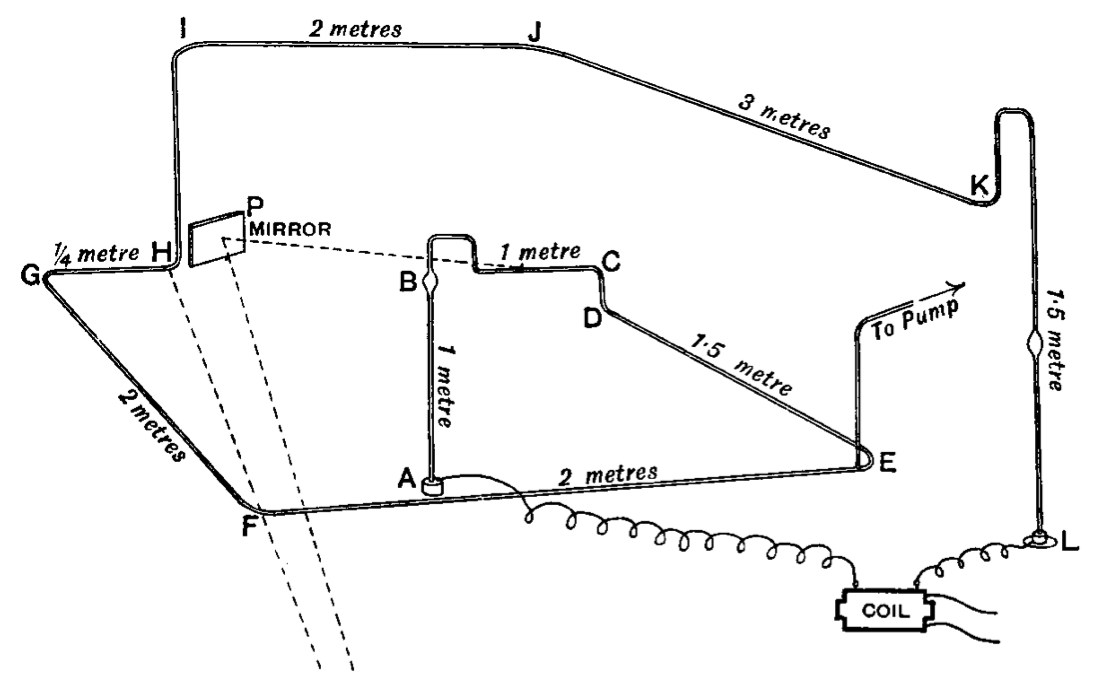
\includegraphics[width=4in]{chapters/introduction/figures/thomson.png}
  \caption{A sketch of J.J. Thomson's early experiments on fast ionization
  waves in long vacuum tubes.}\label{fig:thomson}
\end{figure}
Also using the rotating mirror apparatus, Thomson was able to greatly improve on
the estimates of Wheatstone. He estimated that the so-called ``luminous front''
had a speed that was more than $1.5\times10^{10}$, or in excess of half of the
speed of light. Furthermore, Thomson determined that the front always appeared
to travel from the positively pulsed electrode (anode) to the ground electrode
(cathode).

The study of these luminous fronts was revisited by several researchers in the
wake of Thomson \cite{James1904, Whiddington1925, Beams1926} with varied
success. By his own admission, Beams's work in 1926 was done ``hurriedly,''
using a rudimentary Kerr cell. In 1930, Beams returned to the propagation of
light pulses in vacuum tubes with a rotating mirror apparatus \cite{Beams1930}.
In addition to confirming his previous measurements, and those of Thomson, Beams
discovered that the \acs{fiw} always traveled from the electrode with the
highest absolute potential, to the lowest one. In other words, the wave could be
anode or cathode directed, depending on the magnitude of their potentials
relative to ground. Benefiting from an improved understanding of electricity,
namely the existence of electrons and ions, Beams was able to provide the first
hypothesis on the nature of the \acs{fiw}:
\begin{quote}
  In the neighborhood of the electrode $\ldots{}$ the field is very high and
  intense ionization should take place. This ionization due to the large
  difference in mobilities of positive ions, negative ions and electrons
  respectively should result in the establishment of a space charge. This space
  charge, once formed near the high potential electrode $Q$ must move down the
  tube regardless of the polarity of the applied potential because of the
  changes it produces in the field near its edges.
\end{quote}

At about the same time, Schonland and Collens reported on their observations of
lightning \cite{Schonland1933}. Though the general structure and length scale of
lightning is substantially different from the luminous fronts observed by Beams
and Thomson, the two phenomena would later prove to be very similar. In their
work Schonland and Collens noted that lightning would usually occur in a
two-step process. Based on the images they obtained, they suggested that
the leader was generated by a relatively small ``dart'' with a mean vertical
velocity of $7.2\times10^8$ cm/s. The dart moved in a random manner, changing
directions at random intervals, but always moving downward.

The second step began when this dart reached the ground. Once there, a bright
return stroke would occur along the same path that the leader had traced out. In
contrast to the leader stroke, the return stroke had a velocity of $5\times10^9$
cm/s. Schonland and Collens hesitantly attributed the leader stroke to an
extended electron avalanche, and the return stroke to thermal ionization along
the conductive path generated by the dart. However, calculations by Cravath and
Loeb showed that the speeds of the proposed avalanche would have to be
inconsistent with the fields at the head of a lightning stroke
\cite{Cravath1935}. Instead, they suggested that the dart was actually a moving
region of space charge which locally accelerated electrons to ionizing energies.
This was fundamentally similar to the mechanism proposed by Beams in 1930.

\subsection{The Streamer Model}

It was long known that sparks in air were similar to lightning. Advances in
technology during the 1930's led to experiments which reinforced this
similarity. In response to the measurements of Schonland and Collens; Snoddy,
Beams, and Dietrich studied the breakdown of gas in a long tube with an
oscillograph \cite{Snoddy1936}. The results from the oscillograph showed a very
clear return wave for which they measured several parameters the characterized
as a function of pressure and applied potential. They observed that at low
voltages, the system behaved like a large resistor in series with a capacitor,
and below a critical voltage, no return stroke would form. Finally, in order to
explain the propagation of the \acs{fiw} generated by the positive pulse, they
suggested that photoionization was occurring in the space ahead of the wave.

Around the same time, Flegler and Raether had come to a similar conclusion,
leading to the first attempt at a theory describing streamers
\cite{Flegler1936}. This same theory was proposed independently by Loeb and Meek
in a series of papers \cite{Loeb1940, Loeb1940a, Meek1940}. The streamer theory
divided the initial breakdown of a spark into two steps. In the first step, an
electron avalanche is initiated between two electrodes. The avalanche travels
toward the anode and leaves behind a region of high positive space charge. In
the second step, the return stroke begins at the cathode and travels toward the
cathode. It was suggested that the head of the return stroke ionizes the gas
ahead of it by pulling in background electrons or via photoionization.
\footnote{These early works emphasized the importance of photoionization. It is
now know that it is only required for cathode-directed streamers in systems with
no background ionization. In addition, Mesyats later showed that the lifetime of
the excited states responsible for photoionization were often longer than the
lifetime of the streamers \cite{Mesyats1972}}.

The streamer model proved relatively successful in describing the development of
sparks and lightning. Theoretical estimates of the speed matched the velocity
measurements that were acquired through photographs and oscillographs.
Additionally, the theory is able to account for the halting manner in which
lightning is formed, though it is only tentatively able to describe the
branching and stepped appearance. Finally, the streamer mechanism provides an
adequate explanation of why streamer discharges are not affected by the shape or
material of the cathode, namely, they do not depend on secondary electron
emission.

The study of the formation of streamers and lightning continues to be active to
this day. Following the initial work of Flegler, Raether, Loeb, and Meek, a
number of researchers began to explore the boundary between the Townsend
mechanism and the streamer mechanism. Most notable was Fisher and Bederson's
work in 1951 \cite{Fisher1951}, which was later extended to nitrogen
\cite{Kachickas1952} and argon \cite{Kachickas1953}. However, there were still a
number of phenomena that were poorly explained by the streamer model. In
particular, Kunhardt provided a useful overview of the problems in 1980
\cite{Kunhardt1980}. However, even before that, it was apparent that the
transients of sparks and lightning was more complicated than thought.

\subsection{Ionizing Waves of Potential Gradient}

Per Chalmers \cite{Chalmers1971}, Rogowski and Buss \cite{Rogowski1927,
Buss1932} observed a fast, diffuse, glow discharge immediately prior to the
filaments which often accompany a streamer discharge. Allibone and Meek, noted
similar diffuse discharges in air based on oscillographs and photographs
\cite{Allibone1938, Allibone1938b, Allibone1938c}. However, the Boys apparatus
which was employed in these studies (an ancestor to the modern streak camera)
was unable to capture the evolution of the diffuse glow, given its large spatial
extent.

This was first noted by Allibone who attempted to use Lichtenberg
figures\footnote{Such figures directly exposed photographic emulsions to the
electrical discharge. The developed image was a time-integrated representation
of the discharge.} to definitively capture this diffuse glow
\cite{Allibone1948}. Later, Saxe and Meek used the recently invented
photomultiplier tube to record the evolution of the light emissions in the
brief, diffuse glow \cite{Saxe1948} as a function of space. Both studies
agreed in the existence of the diffuse glow, despite some disagreement on the
nature of its geometry and propagation.

The similarity of fast transient ionization waves in certain glow discharges
\cite{Westberg1959} to those observed in lightning and streamers led Loeb to to
the conclusion that they were all the same phenomena \cite{Loeb1965}. He
referred to them as ``ionizing waves of potential gradient,'' as the proposed
mechanism for the waves was the generation of a steep potential gradient in a
sufficient short period of time. 

As reported by Babich, Loika, and Tarasova \cite{Babich1977}, the detection of
x-ray emissions from pulsed, high-pressure, helium discharges created a new
avenue of interest for these transient plasmas \cite{Stankevich1967,
Noggle1968}. Unlike the streamers, which were often filamentary, these new
discharges exhibited surprising uniformity. The primary difference being the
duration of the pulse (on the order of nanoseconds) and the applied potentials
(in excess of 200 kV).

The x-rays suggested that electrons in these discharges were accelerated to
unusually high energies (on the order of 10 keV) despite the high
collisionality. It was then that Babich and Stankevich suggested that the x-rays
resulted from continually accelerated electrons impinging on the metal
electrodes \cite{Babich1973}. Briefly, the electric fields in the fronts of the
ionizing waves were so large that they managed to accelerate electrons past the
peak in their collisional cross sections.

Mesyats, Bychov, and Kremnev attempted to provide a more rigorous explanation
for the uniform nature of these new discharges \cite{Mesyats1972}. After
conducting several experiments, they came to the conclusion that these transient
plasmas were the result of many overlapping avalanches, unlike the streamer
which only involves a single avalanche. Kunhardt and Byszewski later
expanded on this work by developing a kinetic model to explain the behavior of
all pulsed discharges above the Townsend threshold \cite{Kunhardt1980}.

It was based on the studies of the fast electrons in these discharges that
Mesyats, Bychov, and Kremnev proposed the use of a fast electron beam for
pumping high-pressure gas lasers. Similar work was conducted simultaneously by
Fenstermacher et al.~\cite{Fenstermacher1972}. Palmer \cite{Palmer1974}, and
Levatter and Lin \cite{Levatter1980} determined that there was a threshold
amount of preionization required to ensure homogeneity of the discharge. Hunter
\cite{Hunter1976}, and Koval'chuk and Mesyats \cite{Koval'chuk1976} later
proposed that such discharges be used for fast-closing switches. Gas lasers and
fast switches would drive much of the later research on fast, pulsed discharges.

Eventually these discharges came to be referred to as fast ionization waves
(\acs{fiw}s). A large body of Russian literature developed around their study,
though much of it has remained untranslated. In 1994, Vasilyak produced an
extensive review of these studies \cite{Vasilyak1994}. The data include wave
velocities for a variety of gases and pressures. Other parameters such as
attenuation coefficients for the waves, high energy electron currents, electric
field measurements, and a circuit model of the \acs{fiw} are also included.

\subsection{\textsc{rpnd}s}

Beginning in 1998, the Moscow Institute of Physics and Technology (\acs{mipt})
produced a flurry of studies on the \acs{fiw} \cite{Anikin1998, Pancheshnyi1998,
Starikovskaia1998}. They employed several different diagnostic techniques
(photomultiplier tubes and capacitive probes) in an exceptionally detailed study
in both air and nitrogen, using a shock tube and a bell jar. A summary of these
investigations can be found in \cite{Starikovskaia2001}. The work showed
exceptionally reproducibility of the discharge parameters at relatively low
repetition rates, on the order of tens of Hz, and evidence of runaway electrons.
This work also included some of the first approximations of the electron energy
distribution function (\acs{eedf}).

Interestingly, later analysis of a anode-directed \acs{fiw} in nitrogen by the
group at \acs{mipt} \cite{Pancheshnyi1999} concluded that the, the vast majority
of the electrons were generated \emph{after} the wave. This suggests that the
ionization in an \acs{fiw} does not strictly track the luminous front of the
wave. Additionally, measurements of the conductivity suggested that the local
approximation becomes invalid in the wave front and the electron energy
distribution function resembles a beam.

In 1997 the invention of the fast ionization dynistor (\acs{fid}) was revealed
\cite{Efanov1997}. These new devices enabled sub-nanosecond switching of 10's of
kilovolts, with repetition rates approaching 100 kilohertz. This was a leap
forward over previous technologies which generally used thyristors or spark gaps
for switching. Particularly appealing was the high repetition rate of the
\acs{fid}.

Recall that the volume-filling \acs{fiw} required a significant
amount of preionization. This was often accomplished an ionization source in
addition to the high voltage pulse (in the form of UV radiation, or electron
beams). However, the repetition rates of \acs{fid}s were high enough such that a
substantial number of electrons would carry over between pulses. These seed
electrons obviated the need for a preionization. In addition, the time-averaged
densities of excited states could maintained at much higher values. This had
particular promise for processing applications.

In the eventual commercialization of the \acs{fid} made economically feasible to
create fast, repeatable fast ionization waves. It is this class of discharges
which are now referred to as repetitively-pulsed nanosecond discharges, or
\acs{rpnd}s. Their uniformity, low gas heating, high-pressure operation, and
efficient ionization made them attractive or a number of applications:
\begin{itemize}
  \item plasma-assisted combustion \cite{Starikovskaia2006},
  \item magneto-hydrodynamic energy bypass \cite{Macheret2002},
  \item plasma actuators \cite{Adamovich2009},
  \item and high-pressure xenon lamps \cite{Nikandrov2008, Tsendin2009}.
\end{itemize}

As with the \acs{fiw}s, the primary diagnostics were current and voltage
characteristics, electric field measurements with capacitive probes, and
emission measurements with photomultiplier tubes. Later, intensified \acs{ccd}s
were used to record the emissions of specific transitions as well as broadband
light. This approach has been used to more clearly illustrate the uniformity and
reproducibility of the discharge \cite{Adamovich2009}. Other researchers have
turned to laser-based diagnostics, such as coherent anti-Stokes Raman
scattering, to measure gas heating \cite{Zuzeek2010} and the electric field in
molecular systems \cite{Ito2010, Ito2010a}. Likewise, laser collision-induced
fluorescence (\acs{lcif}) has been used to obtain axial profiles of excited
state and electron densities in helium \acs{rpnd}s \cite{Weatherford2012}.

Concurrent with these improvements in experimental techniques has been similar
progress in the simulation of \textsc{rpnd}s. The one-dimensional models 


  
  \chapter{Theory}\label{chp:theory}
    In order to properly understand the \acs{rpnd}--the experimental measurements,
and the models, it is necessary to develop a theoretical underpinning. The
\acs{rpnd} is an ionized gas, and, dependent on its characteristics, a plasma.
Therefore, we begin with a review of the statistical description of an ionized
gas, equilibrium solutions, and several approximations. Subsequently, the
discharge initiation process is considered from the perspective of a single
avalanche. The Townsend model is briefly reviewed, followed by a more detailed
explanation of the streamer model. This naturally leads to the development of a
homogeneous discharge condition based on the preionization density--the basis
for the \acs{rpnd}. Following this, a qualitative introduction to atomic
structure is provided in order to introduce spectroscopic concepts such as
energy levels, transitions, lineshapes, and absorption cross sections.

\section{Ionized Gas}
An ionized gas is a volume of gas in which some fraction of the neutral atoms
and/or molecules have been separated into electron and ion pairs. For a
sufficiently large number of particles and collision rate, the behavior of each
species in the ionized gas can be described by a continuous distribution
function.

This function is an expression of the likelihood of finding a particle within a
specific range of velocities in a specific volume, as a function of time. This
function is denoted as $f_\alpha(\vec{r}, \vec{v}, t)$, where the subscript
$\alpha$ denotes the species, $f$ is the distribution function, $\vec{r}$ is the
position, $\vec{v}$ is the velocity, and $t$ is the time.

The behavior of $f_\alpha$ can be shown \cite{Bellan2008} to be governed by the
Boltzmann equation,
\begin{equation}\label{eq:boltzmann}
  \frac{\partial f_\alpha}{\partial t} + \vec{v}\cdot\nabla f_\alpha +
  \frac{q_\alpha}{m_\alpha} \left(\vec{E} + \vec{v}\times\vec{B}\right)
  \cdot \nabla_v f_\alpha = \left( \frac{\partial f_\alpha}
  {\partial t}\right)_\mathrm{coll}.
\end{equation}
Here, $m$ is the particle mass, $q$ is its charg:, $\vec{E}$ is the electric
field, $\vec{B}$ is the magnetic field, and $(\partial f_\alpha/\partial
t)_\mathrm{coll}$ is a term which represents changes to the distribution
function as a result of collisions. Coupled with Maxwell's equations,
equation~\ref{eq:boltzmann} provides a complete description of the behavior of
the fields and particles in a plasma.

For a species in equilibrium in the absence of external forces and ($\partial
f_\alpha/\partial t)_\mathrm{coll} = 0$, it can be shown \cite{Druyvesteyn1940}
that the distribution of energies is
\begin{equation}\label{eq:mb}
  f\alpha(\epsilon) = C \epsilon^{1/2}
          \exp\left( -\frac{\epsilon}{\kB T_\alpha}\right)
\end{equation}
where $C$ is a normalizing constant, $\epsilon$ is the energy, $\kB$ is
Boltzmann's constant, and $T_\alpha$ is the temperature of the species. This is
referred to as the Maxwell-Boltzmann distribution. It should be emphasized that
this solution only applies when the classical species can be considered to be in
equilibrium. Gradients and electromagnetic fields can both significantly alter
the distribution function of a species. This can be of particular importance in
the calculation or reaction rates, or the measurement of temperatures.

Additionally, the Boltzmann equation may be solved for electrons in equilibrium
constant electric field, provided that a constant current density, and only
elastic collisions. This is generally valid if the electric field strength is
sufficiently small such that the mean energy of the electrons does not become
comparable to the threshold energies for inelastic collisions. This result was
originally presented by Druyvesteyn and Penning \cite{Druyvesteyn1940} and has
come to be known as the Druyvesteyn distribution. It is defined as,
\begin{equation}
  f_\alpha(\epsilon) = C \epsilon^{1/2}
           \exp\left(-\frac{\epsilon^2}{\langle \epsilon \rangle^2} \right)
  \label{eq:druy}
\end{equation}
where $\langle\epsilon\rangle$ is some mean energy, determined by the gas
properties. This solution tends to suppress the probability of higher and
lower-energy electrons in favor of more intermediate values.
Figure~\ref{fig:simpledists}
\begin{figure}
  \centering
  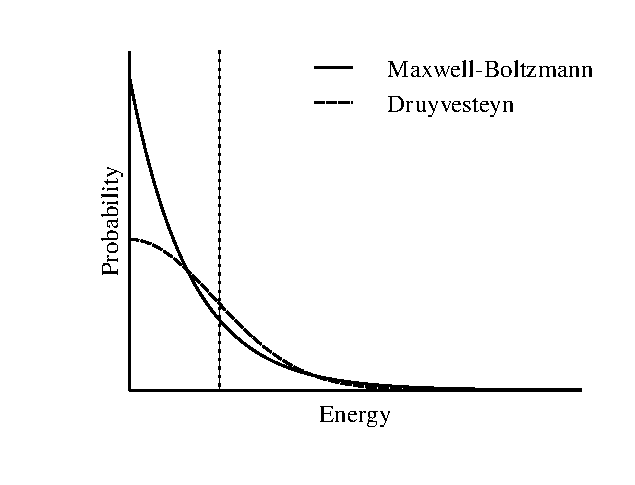
\includegraphics{./chapters/theory/figures/simpledists.eps}
  \caption{Comparison of the Maxwell-Boltzmann energy distribution and the
    Druyvesteyn distribution for the same average energy (illustrated by the
  dotted line).}
  \label{fig:simpledists}
\end{figure}
compares the probability distributions from equations~\ref{eq:mb}
a]nd~\ref{eq:druy} for the same temperature $T_\alpha$. The dotted line
illustrates the average energy for the two distributions, which is not the same
as the most probably energy.

Additional solutions of equation~\ref{eq:boltzmann} in anything but these simple
cases can be very challenging (c.f.\ chapter 18 of \cite{Lieberman2005}). Even
computational approaches can be stymied by the seven-dimension phase space and
high dynamic range. In most situations, the Boltzmann equation is reduced to
more tenable expressions by integrating over velocity-space (leaving $f$ as a
function of space and time). The first so-called moment is the conservation
equation or continuity equation \cite{Lieberman2005},
\begin{equation}\label{eq:cont}
  \frac{\partial n_\alpha}{\partial t} + \nabla \cdot (n_\alpha \vec{u_\alpha})
  = G_\alpha - L_\alpha.
\end{equation}
In this case, there is now a mean velocity $\vec{u}$, as well as gain ($G$) and
loss ($L$) terms which replace the collision operator. The gain and loss terms
are generally expressed as the product of the densities of the interacting
species, and a rate coefficient. For an electron-impact interaction where the
target is relatively stationary, the rate coefficient is
\begin{equation}
  K = \int_0^\infty f_e(\epsilon)\sigma(\epsilon)
      \sqrt{\frac{2\epsilon}{m_e}}d\epsilon,
\end{equation}
where $\sigma$ is the energy-dependent cross section.

The definition of the mean velocity, $\vec{u}$ can be obtained by multiplying
equation~\ref{eq:boltzmann} by $v$ and integrating over velocity-space, to
obtain the second moment \cite{Lieberman2005},
\begin{equation}
  m_\alpha n_\alpha \left[ \frac{\partial \vec{u_\alpha}}{\partial t}
  + (\vec{u_\alpha} \cdot \nabla) \vec{u_\alpha}\right]
  = q_\alpha n_\alpha (\vec{E} + \vec{u_\alpha} \times \vec{B})
  - \nabla \cdot \vec{\Pi} + \vec{f}|_\mathrm{coll}.
  \label{eq:momentum}
\end{equation}
This expresses the conservation of momentum by the plasma. It provides a means
by which to solve for the mean velocity of the system, however it also
introduces two additional terms. $\vec{f}|_\mathrm{coll}$ deals with the forces
transferred to $\alpha$ via collisions. This is often approximated as the Krook
collision operator, which is only dependent on known quantities: $m$, $n$,
$\vec{u}$, $G$, $L$, and the momentum transfer frequency, $\nu_\mathrm{m}$, for
the species $\alpha$ and all species it interacts with. The second term,
$\vec{\Pi}$, is the pressure tensor and can only be defined by the third moment
of the Boltzmann equation. In fact, each additional moment introduces a new term
requiring a higher order moment, \emph{ad infinitum}. In most situations, this
chain of equations is terminated after the first two or three moments by the use
of an additional assumption such as an equation of state. One common example of
an equation of state is the isothermal relation, $p = n\kB T$, which can be used
to remove the pressure tensor.

For the purposes of this paper, one more moment will suffice. Assuming that the
pressure is isotropic, one can multiply equation~\ref{eq:boltzmann} by $mv^2/2$,
and integrate over velocity-space to find the energy conservation equation,
\begin{equation}
  \frac{\partial}{\partial t}\left(\frac{3}{2}p_\alpha\right) 
  + \nabla\cdot\frac{3}{2} (p_\alpha\vec{u}_\alpha)
  + p_\alpha\nabla\cdot\vec{u}_\alpha
  + \nabla\cdot\vec{q}_\alpha
  = \frac{\partial}{\partial
  t}\left(\frac{3}{2}p_\alpha\right)\bigg|_\mathrm{coll}.
  \label{eq:energy}
\end{equation}
In this case, $p$ represents the isotropic pressure, and $\vec{q}$ is the heat
flow. The first term on the LHS represents the total energy contained by the
species, the second term is the energy flux in and out of the volume, and the
third term accounts for changes due to compression or expansion. The RHS is the
collision operator which describes energy added or removed from the system as a
result of collisions.

Equations~\ref{eq:cont} and~\ref{eq:energy} are particularly important for this
study. As will be detailed in chapter~\ref{chp:modeling}, the two can be used to
create a global model of the plasma. Such a model assumes spatial homogeneity of
the plasma in order to reduce the associated computational costs. This allows
the model to address large numbers of species over long periods of time as will
be required in the case of the \acs{rpnd}.

\section{Plasma Criteria}
Though the Boltzmann equation describes both an ionized gas and a plasma, the
two are distinct as a plasma is necessarily an ionized gas, but not vice versa.
A plasma is unique in that its dynamics are governed by long range
electromagnetic forces, unlike gases in which short-range collisions dominate.
As a result, plasmas frequently exhibit large scale structure and organization.
Examples of these structures are ubiquitous in astronomy where phenomena such as
the aurora borealis, coronal mass ejections, and even interstellar media are all
plasmas \cite{Chen1984}. There are three criteria which form a more exact
definition of what constitutes a plasma.

\subsection{Debye Length}
If an electrical perturbation is introduced into an ionized gas, the charged
particles will tend to rearrange themselves to shield it out. A plasma is an
ionized gas which is large enough for this shielding effect to occur. The
characteristic length scale for this shielding effect to take place is referred
to as the Debye length, denoted $\lambda_D$. It can be shown to be equal to
$\sqrt{\epsilon_0T_e/(en_0)}$, where $\epsilon_0$ is the vacuum permittivity,
$T_e$ is the electron temperature, and $n_0$ is the plasma density. If the
characteristic length scale of the ionized gas is $L$, then $\lambda_D < L$ for
it to be considered a plasma.

\subsection{Debye Sphere}
However, the above condition by itself is not sufficient for shielding to occur.
It is possible that an ionized gas may have a relatively small Debye length, but
also lack enough charged particles for shielding to occur. More simply put, it
would be impossible for a single electron to shield out even the smallest of
perturbations. For that reason, the number of particles in a Debye sphere must
be greater than unity in a plasma, or $n_0(4\pi \lambda_D^3/3) >>
1$.\footnote{This condition is also implied in the derivation of the Debye
length.}

\subsection{Plasma Oscillations}
Finally, a plasma may exhibit Debye shielding, but lack the collective behavior
of a plasma. This can occur when the collision frequency with neutral particles
is too high. In this case, the behavior of the ionized gas would be determined
more by the random collisions. Therefore, the characteristic response frequency
of a plasma, commonly called the plasma frequency, must be greater than the
neutral collision frequency, or {$\omega_p > \nu$}. The plasma frequency can be
shown to be $\omega_p = \sqrt{e^2n_0/(\epsilon_0 m_e)}$.

There are many natural and man-made plasmas of varying size and quality.
Figure~\ref{fig:regimes}
\begin{figure}
  \centering
  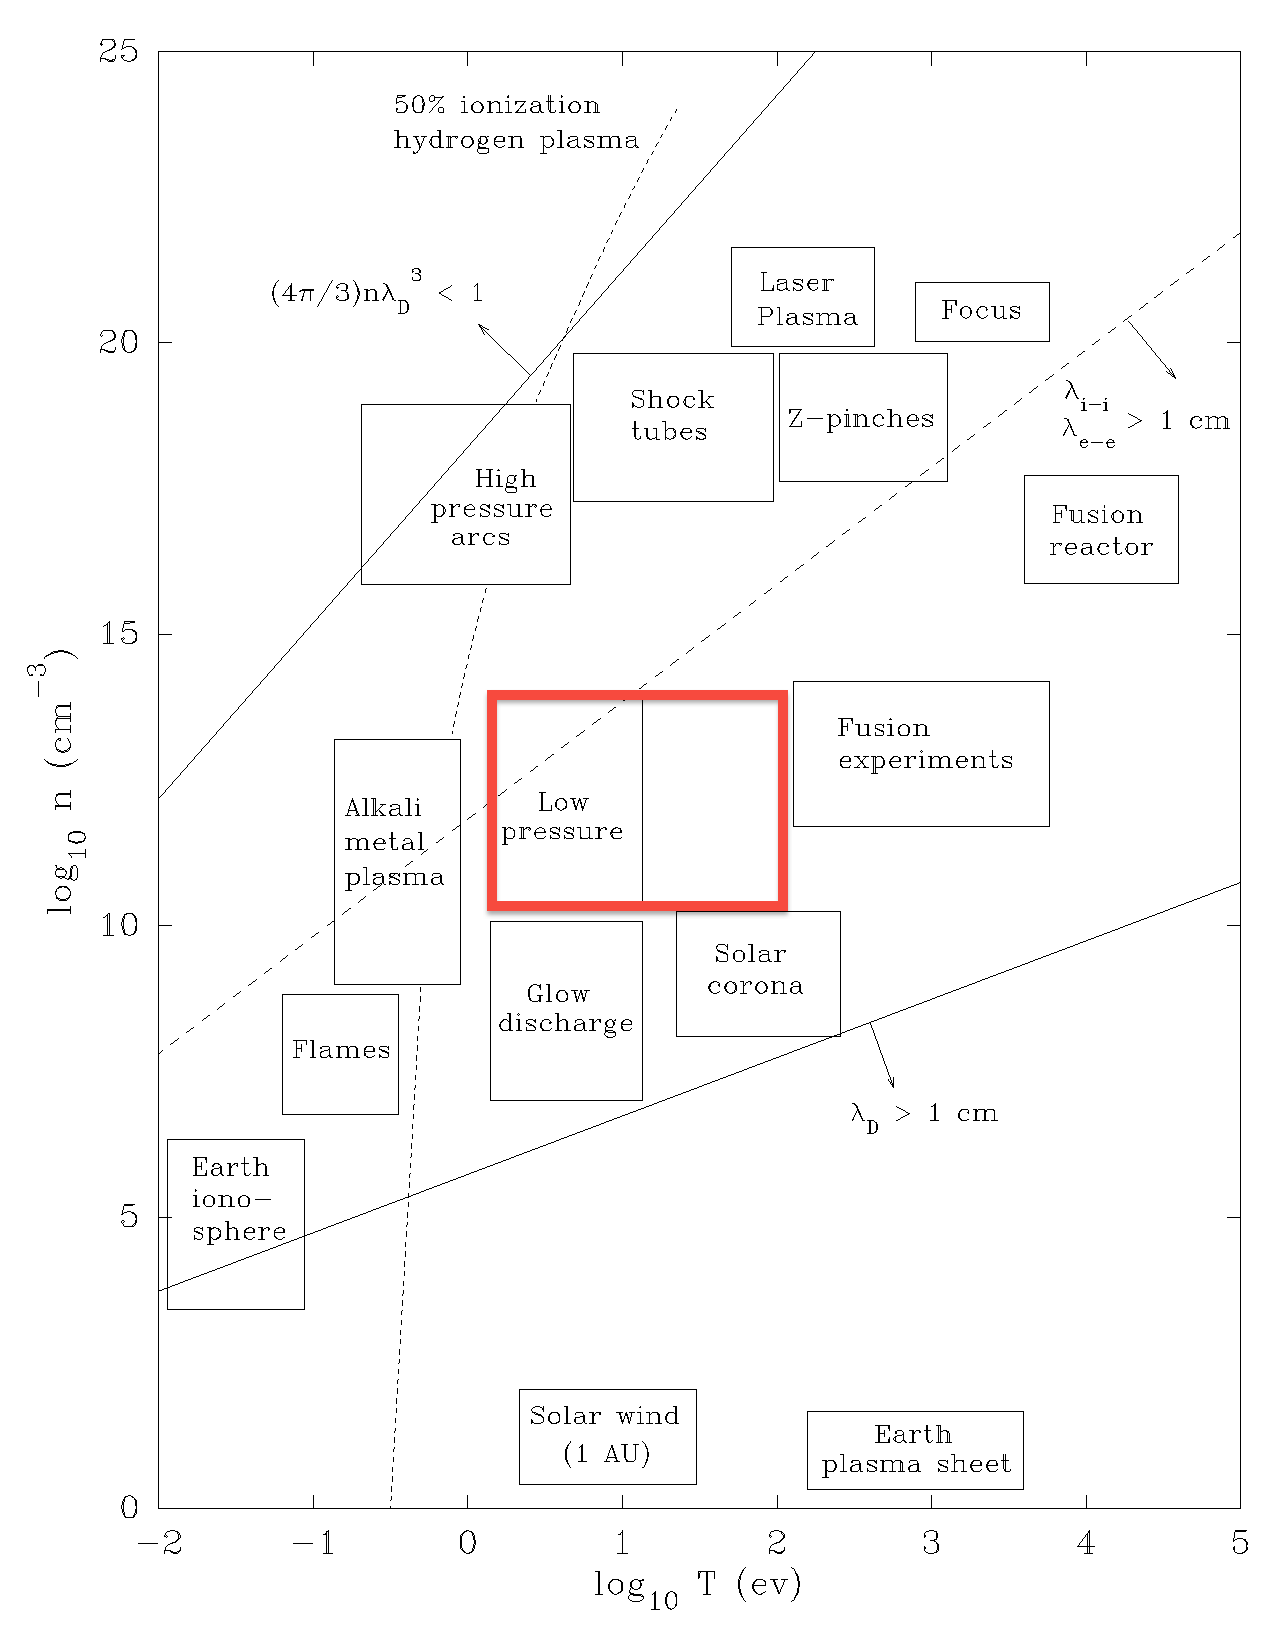
\includegraphics{./chapters/theory/figures/regimes.pdf}
  \caption{Illustration of the various regimes of plasma in terms of
    electron temperature and density with the \acs{rpnd} regime highlighted,
    adapted from \cite{Huba2011}.}
  \label{fig:regimes}
\end{figure}
shows several categories of plasma, plotted as a function of their electron
density and temperature. As can be seen in this example, the electron densities
span seven decades, and the densities cover in excess of 20. This broad range of
conditions presents a particularly challenging problem for both simulations and
experimental measurements. Also highlighted in the figure is the range spanned
by the \acs{rpnd}.

\section{Discharge Initiation}
The Boltzmann equation is a continuous, statistical description of a plasma. By
comparison, the initial breakdown of a plasma is a highly discontinuous process
marked by its stochasticity. The initiation of a discharge is typically the
result of electron avalanches which occur randomly throughout a volume of gas
\cite{Druyvesteyn1940}. Often, the seed electrons for a plasma are the products
of ionizing cosmic rays. At sea level this results in a few electrons per
cubic-centimeter. As a result, it is necessary to consider the initiation of a
discharge separately from a pre-existing plasma.

\subsection{Townsend Mechanism}

Classically, plasmas are created by two different mechanisms, the applicability
of which depends on primarily on the strength of the electric field relative to
the neutral gas density, a value called the reduced electric field
\cite{Huxley1966}. At lower reduced fields, the Townsend mechanism is
responsible for the formation of a plasma. Consider two electrodes separated by
a gap filled with some gas. An electron starting near the cathode will drift
toward the anode. For a large enough electric field, the electron will gain
sufficient kinetic energy to ionize a neutral atom, producing a second electron.
The two electrons are now accelerated by the field, instigating further
ionization of the background gas. The population of electrons quickly grows,
thus the process is referred to as an electron avalanche. Eventually, the
avalanche electrons are collected at the anode.

In their wake are ions which slowly drift toward the cathode. As the ions impact
the surface of the cathode, they occasionally cause a secondary electron to be
emitted. This secondary electron initiates a new avalanche and helps to sustain
the discharge. A steady state electric discharge occurs when the current of the
ion collection at the cathode matches the current of the electron collection at
the anode. The time scale of the Townsend discharge is usually determined by the
positive ions, as their large mass results in slow drift velocities. For an
electric field of 50 V/cm at 200 mTorr, the drift velocity of a helium ion in
helium is about $7\times10^4$ cm/s \cite{Hornbeck1951}. For a gap of 10 cm, this
gives a drift time on the order of $10{-4}$ s.

The Townsend mechanism is characterized by two parameters: $\alpha$ and
$\gamma$, the first and second Townsend coefficients. $\alpha$ is the number of
ionization events that occur per unit length, often expressed as a function of
the reduced field \cite{Druyvesteyn1940}. The second Townsend coefficient is the
probability that an ion impinging on the cathode produces a secondary electron.
The values for $\gamma$ can vary widely and depends on the type of ion, its
energy, the cathode material, contamination of the surface, and many other
factors. That said, typical values are around 0.01-0.1 \cite{Lieberman2005}.

\subsection{Streamer Mechanism}

In contrast, the streamer discharge which occurs for larger values of the
reduced field does not depend on secondary emission. Additionally, streamer
discharges can develop in time periods as short as 1 ns, much less than the time
required for Townsend breakdown. In order to describe the streamer mechanism,
again consider an electron between two electrodes, as seen in (a) of
figure~\ref{fig:streamer}.
\begin{figure}
  \centering
  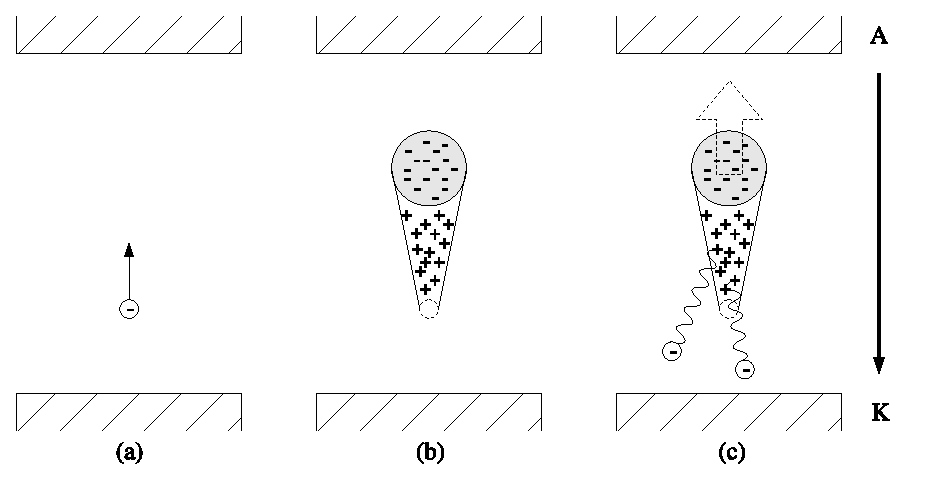
\includegraphics{./chapters/theory/figures/streamer.eps}
  \caption{An illustration of the development of a single streamer. (a)
    A seed electron is accelerated by the applied electric field. (b) The
    initial electron develops into an avalanche which leaves a large region
    of positive space charge, slowing further advance. (c) The streamer
    propagates toward the cathode via photoionization and the anode via
    nonlocal electrons and photoionization. Adapted from \cite{Levatter1980} and
    \cite{Kunhardt1980}.}
  \label{fig:streamer}
\end{figure}
As with the Townsend discharge, this electron initiates an avalanche which moves
toward the anode. As the electrons travel toward the anode, they randomly
collide and diffuse, leaving behind a cone of ions, as seen in part (b).
However, the higher reduced field drastically increases $\alpha$. This causes
the space charge of the avalanche to create an electric field comparable to the
one that is applied, slowing the propagation of the avalanche.

At this point the avalanche can be considered a streamer as it begins to
increase its extent by several additional processes. The large internal fields
of the avalanche can accelerate individual electrons and ``inject'' them in the
direction of the anode \cite{Kunhardt1980}. In addition, as the excited atoms in
the wake of the avalanche begin to radiate, they can cause photoionization
throughout the volume. Photoelectrons generated close enough to the negative
head, or positive tail of the streamer will initiate secondary avalanches which
eventually connect to the primary one. While photoelectrons may cause some
additional broadening of the streamer, the injection of electrons toward the
anode is aligned with the direction of the internal field of the avalanche. As a
result, the ionization caused by these electrons do not appreciably increase the
radius of the streamer.

\subsection{Homogeneity Condition}

However, these processes are not critical in the formation of a large-volume
discharge by an \acs{rpnd}. This description of a streamer only considers an
avalanche generated by a single electron. In reality, many can form
simultaneously assuming that there is more than one seed electron in the volume.
With moderate preionization of the volume, the strong fields of the individual
avalanches can begin to overlap\footnote{If the preionization of the volume is
too large, it can effectively short out the electric field.}. This smoothes out
the field gradients which would otherwise radially constrict the streamers.
Instead, ionization progresses homogeneously throughout the volume.

In order to determine the necessary preionization density, we refer to the work
done by Levatter and Lin on gas laser discharges \cite{Levatter1980}. First, the
electron drift velocity in an applied field can be expressed as the product of
the field and the electron mobility $\mu$. The electron mobility multiplied by
the electric field is the steady-state drift velocity for an electron in that
field and represents the balance between the frictional force of the neutral gas
collisions and the electric field. Consequently, the mean velocity of electrons
drifting in a time-varying field $E(t)$ can be expressed as
\begin{equation}
  u(t) = \mu(E) E(t).
\end{equation}

The length of the avalanche can be written as a time-integrated function of the
electron drift velocity,
\begin{equation}
  \xi = \int_{t_0}^t u(t) dt.
  \label{eq:s_xi}
\end{equation}
Here, $t_0$ is the time at which $E(t)$ becomes high enough that the first
Townsend coefficient, $\alpha$, exceeds 0. Because no electron multiplication
occurs while $\alpha < 0$, this effectively represents the beginning of the
avalanche.

The electric field in the head of the avalanche depends on its radius, which is
dependent on the diffusion of the electrons as they cross the gap. This is
governed by the free diffusion coefficient, $D$. For a fixed diffusion constant,
the final avalanche radius would simply be $R = \sqrt{2D\Delta t}$, where
$\Delta t$ is the time after breakdown. As the diffusion coefficient typically
varies with the applied electric field, the final avalanche radius will be
assumed to be equal to $R = \sqrt{2\bar{D}\Delta t}$, where $\bar{D}$ is the
time-averaged diffusion coefficient.

Levatter and Lin assume that the avalanche slows when the peak field of the
avalanche is equal to the applied field. Assuming that the electrons diffuse
equally in all directions, the electric field of the avalanche head can be
expressed as
\begin{eqnarray}
  E_a(r) = \frac{eN_e}{4\pi\epsilon_0R^2} F(r/R), \qquad \mathrm{where} \\
  F(r/R) = \frac{1}{R^2}\left[\mathrm{erf}(r/R)-\frac{2}{\pi^{1/2}}
           (r/R)\exp(-r^2/R^2)\right] ,
\end{eqnarray}
where $r$ is the radius with respect to the center of the avalanche, $N_e$ is
the number of electrons in the avalanche, $\mathrm{erf}$ is the error function.
$F$ is a dimenionless function which has a peak value of $0.428$. Provided
$\alpha$ as a function of reduced field, the number of electrons in the
avalanche is equal to
\begin{equation}
  N_e = \int_0^\xi \alpha(\xi')d\xi'.
  \label{eq:s_pop}
\end{equation}

Here, Levatter and Lin make a number of assumptions in order to develop an
analytic and dimensionless solution for $E_{a,\mathrm{max}}(t) = E(t)$. However,
it is possible to numerically integrate equations~\ref{eq:s_xi},~\ref{eq:s_rad},
and~\ref{eq:s_pop} to determine the time required for the avalanche to slow.
This should provide a more accurate, but less general result. Assuming a
linearly increasing electric field, figure~\ref{fig:avalanche_lengths}
\begin{figure}
  \centering
  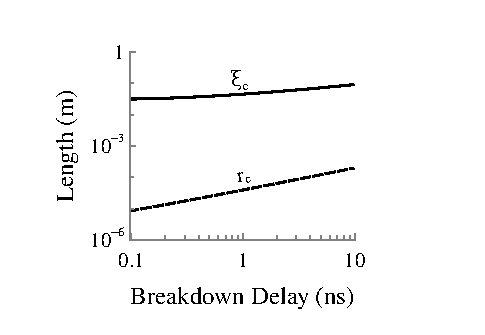
\includegraphics{./chapters/theory/figures/avalanche_lengths.eps}
  \caption{Numerical calculations of the avalanche length and avalanche radius for
    in helium at a pressure of 4.0 Torr as a function of the slope of the electric
    field, $dE/dt$.}
  \label{fig:avalanche_lengths}
\end{figure}
shows the results of such calculations for an avalanche in 4.0 Torr of helium,
as a function of various breakdown delays. The breakdown delay is defined as the
time it takes for $\alpha > 0$. The mobilities, diffusion coefficients, and
Townsend coefficients were interpolated from solutions of the Boltzmann equation
provided by the BOLSIG+ code with Phelps' cross sections \cite{Phelps2002}. For
this range of breakdown delays, the avalanche was able to develop up to nearly
10 cm in length before it slowed. The times required for the avalanche to slow
ranged from around 23 ns for the shortest breakdown delay, and 389 ns for the
longest.

From this, a criteria for homogeneous breakdown of the gas can be developed. In
order for the field gradients to be smoothed out, the individual avalanche heads
should roughly overlap by the time they have slowed. Assuming that all seed
electrons in the volume initiate avalanches, this can be approximated as
$n_{e,c} > r_c^{-3}$, where $n_{e,c}$ is the critical electron density, and
$r_c$ is the avalanche radius when it has slowed. As seen in
figure~\ref{fig:avalanche_densities},
\begin{figure}
  \centering
  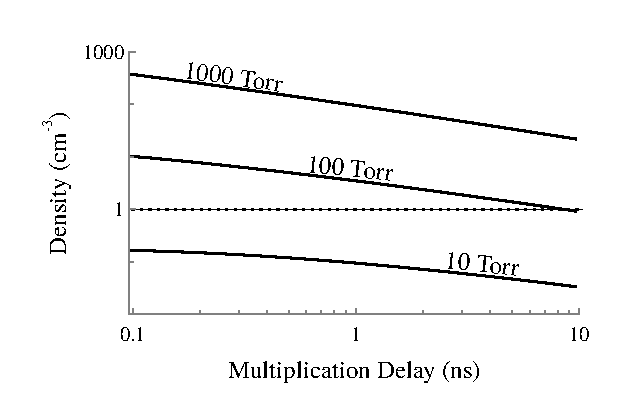
\includegraphics{./chapters/theory/figures/avalanche_densities.eps}
  \caption{Minimum preionization densities required at a variety of pressures
    and breakdown delays. The dotted line indicates the background ionization
    level as a results of cosmic radiation.}
  \label{fig:avalanche_densities}
\end{figure}
the required preionization density depends on both the breakdown delay and the
operating pressure. Generally, the preionization density increases with pressure
and decreases with breakdown delay. The dotted line in the figure indicates the
anticipated background electron density from cosmic radiation. This suggests
that, for the breakdown delays in question, the discharge will almost always be
homogeneous at pressures below 100 Torr. While the plot suggests that large
values of $dE/dt$ might guarantee homogeneous breakdown at near-atmospheric
pressure, the increasing likelihood of ionization instabilities \cite{Johns1972}
will preclude homogeneous discharge development.

\section{Atomic Spectroscopy \& Notation}

As described, much of the experimental work presented will concern the use of
spectroscopic techniques. Careful measurements of the light emitted from excited
atomic states can yield electron densities and temperatures, excited state
densities and temperatures, electric fields, and magnetic fields
\cite{Griem2005}. The topic of spectroscopy is extensive and it is neither
necessary nor desirable to cover it in full. Instead we will only consider what
is necessary to understand the emissions from a singly-excited, multi-electron
atom.

An atom is composed of a small, positively charged nucleus, orbited by
negatively charged electrons. The actual position of any single electron is
probabilistic and described by a wavefunction--solutions of the Schr\"{o}dinger
equation for the atom in question. Each wavefunction is associated with a number
of eigenvalues which quantize aspects of the state of bound electrons. In simple
atoms, four such quantum numbers are of interest \cite{Drake2006},
\begin{itemize}
  \item $n=1,2,\ldots$: the principal quantum number,
  \item $l=0,1,\ldots,n-1$: the orbital angular momentum number,
  \item $m_l =-l,\ldots,l$: the projection of $l$, and
  \item $m_s=\pm1/2$: the projection of the spin quantum number.
\end{itemize}
The quantum numbers are hierarchical such that each $n$, or shell, possesses a
series of subshells, $l$, while each subshell possesses a number of individual
orbital, $m_l$, and each orbital possess one of two spins. As a result of the
Pauli exclusion principle, the wavefunction of each electron around an atom is
described by a \emph{unique} set of quantum numbers. This means, that any
particular subshell can only contain $2(2l+1)$ electrons. The subshells are
often referred to using the nomenclature $0,1,2,3,\ldots = s,p,d,f,\ldots$.

As a result of their separation from the nucleus, the electrons in an atom
possess some degree of potential energy. As the $n$ and $l$ of an electron
increase, so does its potential energy. In the absence of electric and magnetic
fields, $m_l$ and $s$ do not affect the potential energy of an electron. As an
example, an electron in the 1s ($n=1$ and $l=0$) subshell has the lowest
possible potential energy.

Absent from external influences, the individual states are populated with
electrons so as to minimize the total potential energy of the system. This
natural arrangement is referred to as the ground state configuration. Often, but
not always, the subshells are filled sequentially and in order from lowest to
highest $l$ \cite{Drake2006}. Provided some input energy in the form of a
collision or a photon, one or more of the electrons surrounding the atom may
transition to another state, increasing the potential energy of the system. In
low-temperature plasmas it usually one of the electrons from the outermost or
partially filled subshell to be excited.

The potential energies of the electron configurations for multi-electron atoms
are determined by the collective effects of all the surrounding electrons.

It is the collective effects of all electrons surrounding an atom which
determine its potential energy. This results in a single set of total angular
momenta which can be used to describe the atom. In lighter atoms
\cite{Drake2006}, the contributions of the individual electrons are combined
assuming a condition called L-S coupling. Under this assumption, the total
angular momentum of the atom can written as $\vec{L} = \sum\vec{l}_i$, where $i$
is each electron in a partially filled subshell (filled subshells sum to zero).
Likewise, the total spin can be written as $\vec{S} = \sum\vec{s}_i$. These can
be combined to form the total angular momentum of the atom, $\vec{J} = \vec{L} +
\vec{S}$. Finally, the each atom is said to have an even or odd parity, defined
as $(-1)^{\sum\bm{l}_i}$, where $-1$ is odd, and $1$ is even.

These quantities can be used to write a ``term symbol'' for the atom, of the
form $^{2S+1}L_J^p$, where $p$ is `o' if the parity is odd, and omitted if it's
even. The term symbol can be augmented by prepending additional terms which
address the subshells in which electrons can be found. This is typically written
as $nl^N$, where $N$ is the number of electrons in a given subshell (ommitted if
$N=1$). For example, 1s2s$^3$S$_{1}$, describes the triplet helium metastable
state. In this case, there is a single electron in the 1s subshell and a second
atom in the 2s subshell. The configuration has a total orbital angular momentum
of 0 (denoted by the `S'), an even parity (denoted by the absence of a
superscript `o'), a total spin of $1$ (the superscript $3$ is equal to $2S+1$),
and a total angular moment of 1.

Excited atomic states usually have finite lifetimes. Normally, electrons will
undergo transitions to lower the potential energy of the system. This can also
occur spontaneously, through the emission of a photon, or through a superelastic
collision with another particle. In the case of spontaneous transitions, only
certain states can transition to others, as defined by a series of selection
rules \cite{Drake2006}:
\begin{itemize}
  \item $\Delta S = 0$
  \item $\Delta L = \pm1$ or 0
  \item $\Delta J = \pm1$ or 0
  \item $L=0$ cannot transition to $L=0$
  \item $j=0$ cannot transition to $J=0$
\end{itemize}
These rules are determined from a lower order approximation, and thus are not
strict. As a result, forbidden transitions can occur, however these generally
take place at much lower rates.

Figure~\ref{fig:grotrian}
\begin{figure}
  \centering
  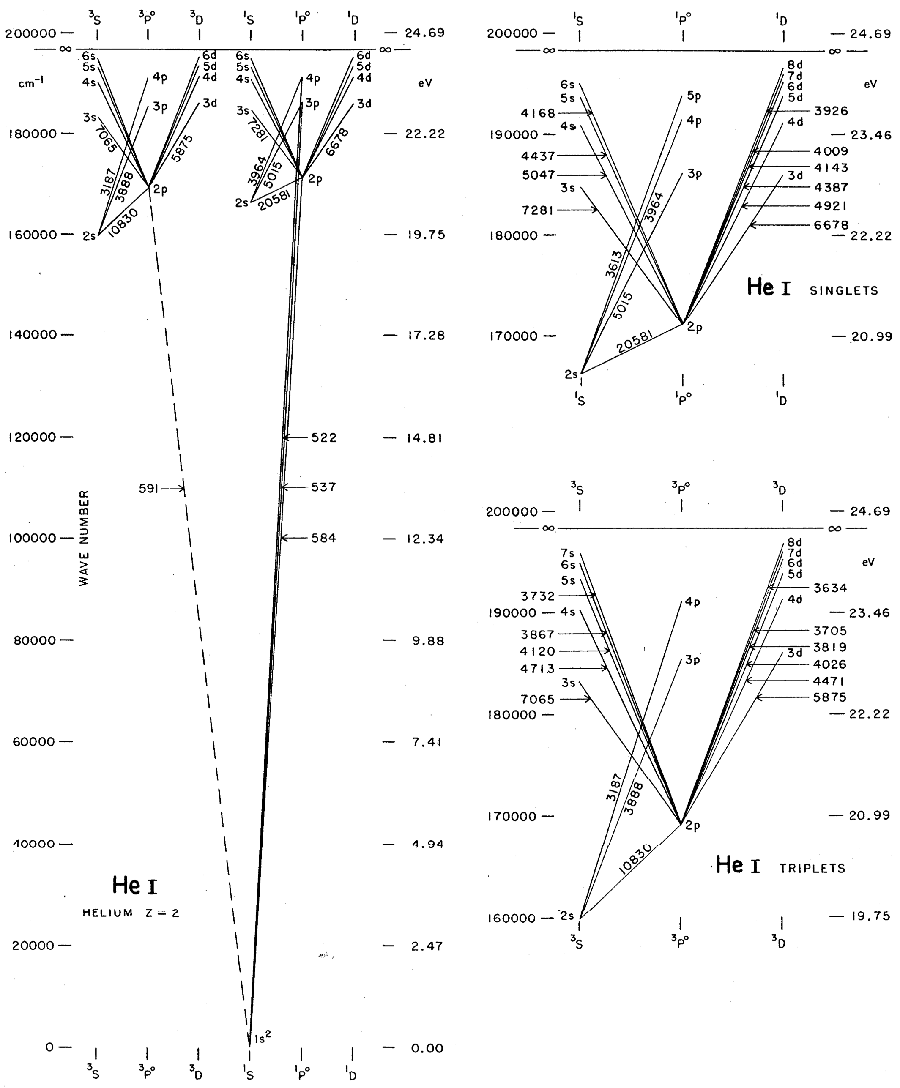
\includegraphics{./chapters/theory/figures/grotrian.pdf}
  \caption{A partial Grotrian diagram of neutral helium, from \cite{Moore1968}.}
  \label{fig:grotrian}
\end{figure}
is a Grotrian diagram of the energy levels in neutral helium and the allowed
transitions. In this case, the atomic states are separated into the singlet
($S=0$) and triplet ($S = 1$) manifolds. The singlet manifold is composed of
excited states where the electron spins are anti-parallel, and the triplet
manifold represents excited states where the electron spins are parallel. As
indicated by the first selection rule, transitions between these two manifolds
is forbidden, thus each is something of a self-contained system
\cite{Herzberg1944}.

Also observable in the diagram are two ``metastable'' states. These are the 2s
states at the bottom of the singlet and triplet manifolds. An electron in either
state cannot spontaneously transition to a lower energy state. As a result, an
electron in either state can be extremely long-lived. In addition, they are also
the lowest-lying excited states of helium. For these reasons, helium plasmas
tend to have high densities of metastable atoms. This makes them a good
candidate for spectroscopic study as will be seen in
chapter~\ref{chp:metastables}.

\subsection{Spectral Lineshapes}

Electrons which transition to lower energy states emit photons which can be
detected. Conversely, if an atom is exposed to a photon with an energy matching
a transition, the atom may absorb the photon. Both processes are useful in
determining the prevalence and dynamics of the excited states. This, in turn,
can be used to infer various plasma properties.

Conservation of energy requires that the energy of the absorbed or emitted
photon match the energy difference between the two states. However, the finite
lifetime of excited atomic states implies, via the time-energy formulation of
the uncertainty principle, some uncertainty in the actual energy difference
between the states. As a result, the emitted photon will possess an energy
selected from a distribution of energies.

This distribution is referred to as the spectral lineshape. The narrowest
permissible lineshape, or natural lineshape, of an atomic transition can be
shown \cite{Siegman1986} to be a Lorentzian of the form,
\begin{equation}
  g(\omega) = -\frac{1}{4\pi^2}\frac{A\lambda^3}{\dwa}
  \frac{1}{1 + \left[2(\omega-\omega_a)/\dwa\right]^2},
  \label{eq:lorentzian}
\end{equation}
where $\omega$ is the photon frequency, $A$ is the Einstein coefficient for the
transition, $\lambda$ is the wavelength of the transition, $\omega_a$ is central
frequency of the transition, and $\dwa$ the full-width half maximum (\acs{fwhm})
of the transition. In the ideal case, where the atoms motionless and unaffected
by external perturbations, $\dwa = A$ \cite{Siegman1986}. This is known as the
natural linewidth.

Other processes can act to broaden or alter the spectral lineshape
\cite{Kunze2009}. For example, inter-atomic collisions can reduce the lifetimes
of excited states. This results in additional broadening of the line, though it
retains its Loretnzian nature. As the frequency of inter-atomic collisions
increases linearly with pressure, this phenomena is referred to as pressure
broadening. It can be included in equation~\ref{eq:lorentzian} by using $\dwa =
A + BP$, where $B$ is a measured or calculated broadening coefficient, and $P$
is the pressure \cite{Siegman1986}.

Atomic motion can also play a role in the spectral lineshape. If an atom is
moving toward or away an observer as it emits a photon, the emitted photon will
be blue or red shifted. Likewise, if the atom is moving toward or away an
incident photon, the energy of that photon will be shifted \cite{Siegman1986}.
If this effect is averaged over the random motion of atoms in a gas, the result
is an additional broadening of the lineshape, called Doppler broadening. Unlike
pressure broadening, Doppler broadening introduces a Gaussian component to the
lineshape such that,
\begin{multline}
  g(\omega) = \sqrt{\frac{2\ln{2}}{\pi^3}}\frac{\dwa}{\dwd}
  \int_{-\infty}^\infty
  \frac{1}{[(\omega - \omega_a) - \omega']^2 + 4\dwa^2} \\
  \times \exp\left[4\ln{2}\left(\frac{\omega'}{\dwd}\right)^2\right]d\omega'.
  \label{eq:voigt}
\end{multline}
Here, $\dwd = \omega_a\sqrt{\frac{8k_\mathrm{B}T_\mathrm{g}\ln{2}} {Mc^2}}$, is
the width of the Doppler broadening, where $T_g$ is the gas temperature, $M$ is
the particle mass, and $c$ is the speed of light. This form of the spectral
lineshape is known as the Voigt profile, and it must be numerically integrated.
In the case that $\dwd >> \dwa$, equation~\ref{eq:voigt} can be simplified to a
standard Gaussian distribution,
\begin{equation}
  g(\omega) = \sqrt{\frac{4\log{2}}{\pi\dwd^2}}
  \exp\left[-(4\log{2})\left(\frac{\omega-\omega_a}{\dwd}\right)^2\right].
\end{equation}

The effect of the various broadening mechanisms is most apparent in the wings of
the lineshape, far from the peak. Figure~\ref{fig:lineshapes}
\begin{figure}
  \centering
  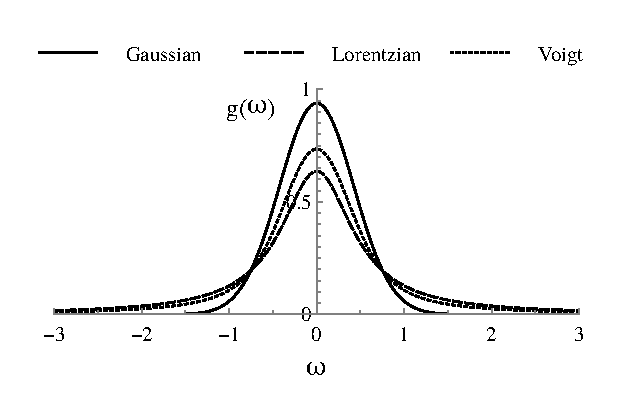
\includegraphics{./chapters/theory/figures/lineshapes.eps}
  \caption{A comparison of the three primary spectral lineshapes, each with the
  same full width.}
  \label{fig:lineshapes}
\end{figure}
illustrates the three major lineshapes with equivalent full widths. The Voigt
profile is composed of equally broad Lorentzian and Gaussian distributions. As
can be seen, the wings of the Gaussian distribution fall off very quickly. In
comparison, the Lorentzian component is observable well out to the edges of the
figure. 

The spectral lineshape can be altered by a number of other processes. Electric
fields can influence the emissions via the Stark effect, while magnetic fields
can split up degenerate states via the Zeeman effect. The fields of electrons
and nearby molecules can also alter the lineshape of a transition. While not
used in this study, such effects can be used as effective diagnostic tools in
the measurement of field strengths, and charged particle densities in plasmas.

\subsection{Absorption}

As has been mentioned, a photon which closely matches the energy between two
states can be absorbed by an atom. This property forms the basis for absorption
spectroscopy where light with a known spectrum is used to illuminate a sample.
The spectrum of the light that passes through the sample is measured and used to
infer properties of the sample. In contrast to the emission processes occur
spontaneously with a characteristic lifetime, often 10s of nanoseconds or more,
absorption is almost instantaneous. This makes absorption-based spectroscopic
methods desirable for fast phenomena, such as the \acs{rpnd}
\cite{Demtroder2008}.

The cross section for a single atom to interact with a photon can be shown
\cite{Siegman1986} to be,
\begin{equation}
  \sigma(\omega) = A \frac{\lambda^2}{8\pi}\frac{g_1}{g_2}g(\omega).
  \label{eq:absorb}
\end{equation}
where $g_1$ and $g_2$ are the number of degenerate configuration for the lower
state and upper state respectively. $g(\omega)$ is the appropriate spectral
lineshape, determined from the operating conditions.

It is important to recognize that absorption spectroscopy can also perturb the
system it is measuring. Suppose two consecutive photons were incident on the
atom. If the first was absorbed, the likelihood that the second photon would be
absorbed is zero. The cross section for absorption has not changed, there are
simply no atoms available for the second photon to interact with. Therefore, if
a photon field is incident on a volume of atoms susceptible to absorption, the
degree to which the field is absorbed will depend on its intensity. The more
intense the photon field is, the more it reduces the number of atoms available
to interact with.

Eventually, this effect is balanced by a process called stimulated emission. In
this process, an atom is already in an excited state with one or more lower
states. If an photon is incident on the atom and matches the energy difference
between its current state and a lower one, the photon may induce a transition to
the lower state. This results in the emission of a second photon with the same
energy and phase as the first. The cross section for stimulated emission is
identical to that for photon absorption.

This feedback process where the absorption and emission processes balance with
each other is known as saturation. The saturation of a volume of gas is a
continuous process, and depends on the atomic states in question and areal
density of the incident photons, or intensity. From a practical standpoint,
absorption measurements require that the interrogating photon field remain below
a threshold value. This saturation intensity can be shown \cite{Siegman1986} to
be,
\begin{equation}
  I_s = \frac{2\sqrt{2}h\nu_0A}{\lambda^2},
\end{equation}
where $h$ is Planck's constant, and $\nu_0$ is the nominal frequency of the
transition \cite{Siegman1986}.

In this report, absorption and spontaneous emission diagnostics provide the
experimental basis on which the \acs{rpnd} analyzed. Both are direct measures of
the excited states that exist within a \acs{rpnd}. However, neither provides any
direct measurement of the quantity or energies of the electrons. In the
\acs{rpnd}, as with all plasmas, the electrons play a fundamental role in how
the discharge behaves and develops. At the most basic level, it is the electrons
which are accelerated by the electric field and collide with the gas atoms to
produce the aforementioned excited states. Consequently, it should be possible
for a sufficiently detailed model to use measurements of the excited states in
order to infer the properties of the electrons, as will be seen in
chapter~\ref{chp:modeling}.


  \chapter{Experiment}\label{chp:experiment}
    \section{Discharge Apparatus}

The design of the discharge apparatus was similar to the coaxial geometry used
by Vasilyak and others \cite{Vasilyak1994}. This configuration has the benefit
of minimizing the inductance of the system, which should aid in the propagation
of the pulse through the system. Figure~\ref{fig:appschem}
\begin{figure}
  \centering
  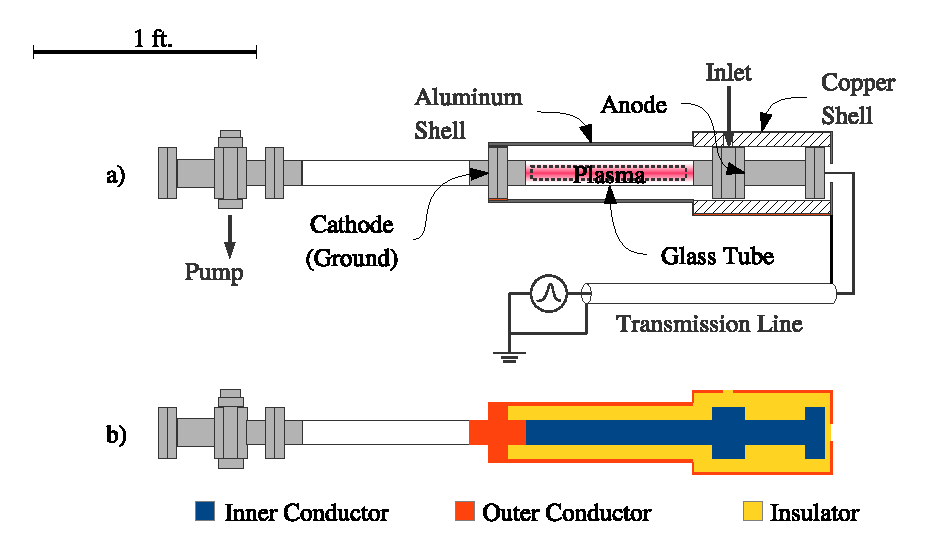
\includegraphics{./chapters/experiment/figures/appschem.eps}
  \caption{A scaled illustration of the discharge apparatus used in the
  \acs{rpnd} experiment.}
  \label{fig:appschem}
\end{figure}
is a to-scale illustration of the discharge apparatus.

The main portion of the discharge was provided by a borosilicate glass tube with
Conflat flanges on either end. The glass portion of the tube had an inner
diameter of 3.3 cm, an outer diameter of 4.0 cm, and a length of 22.9 cm. The
total length of tube, including the glass tube, glass-to-metal transition, and
flanges was 30 cm. The flanges served as the electrodes for the plasma. Seen
here, the anode is located on the right, and the cathode/ground is located on
the left.

The cathode was connected to a second glass tube with the same dimensions as the
first. This tube led to the pumping apparatus and served to electrically isolate
it from the rest of the system. The cathode was also connected to ground through
a cylindrical ground shell\footnote{While all of the outer conductors of the
system are nominally at ground, it is believed that they would float to finite
voltages with each pulse. This is a product of the nonideal impedance to ground
and the high frequencies associated with the fast pulse.} which ran along the
outside of the discharge tube. The ground shell was held in place against the
cathode with a copper shim and Delrin shaft collar.

Two slots were milled into the ground shell on opposite sides. The slots were
3.8 cm by 30 cm and served to provide optical access to the discharge tube. The
side of the ground shell opposite the cathode terminated at a copper sheet, 10
cm square. The copper sheet was perpendicular to the axis of the discharge tube
and had a 5 cm hole for discharge tube to pass through. The ground shell was
connected to the copper sheet with conductive copper tape.

The copper sheet was secured to a Teflon tube, approximately 20 cm in length
with an inner diameter of about 7.5 cm and an outer diameter of 10 cm. The
Teflon tube provided electrical isolation for the anode from structures
supporting it. Surrounding the Teflon tube was a second ground shell composed of
copper. This was connected to the first ground shell by a braided copper strap.
The other end of the second ground shell ended in a similar square copper sheet,
10 cm on each side. This sheet was secured to the Teflon tube by nylon screws
and seated against the ground shell for electrical contact.

The copper sheet also featured a HN bulkhead adapter for connection to the
transmission line. The inner conductor of the bulkhead adapter was connected by
a straight run of 5 cm of silicone-coated wire to a Conflat window angled at
45$^\cdot$. The window was connected to a Conflat nipple, which in turn was
connected to a double-sided flange used as the gas inlet (access was provided by
a 2.54 cm diameter hole drilled into the surrounding Teflon tube). The other
side of the double-sided flange was connected to the anode of the discharge
tube.

The voltage pulse was provided by a \acs{fid} pulser, supplied by \textsc{anvs},
Inc. (model \smaller{PT510NM}). The amplitude of the pulse was fixed at 6.4 kV
with a repetition rate of 1.0 kHz. Each pulse had a fixed width of 25 ns, with a
10\%-90\% rise time of approximately 4 ns and a roughly Gaussian shape. It is
likely that the low conductivity of the gas preceding each pulse resulted in a
doubling of the pulse potential as it reflected from the electrode. A
\textsc{srs} \smaller{DG645} delay generator was used as the master clock in all
experiments and was used to trigger the pulser. A 13.7 m transmission line was
used in order to isolate reflections traveling back and forth between the pulser
and anode. The cable used was RG213, and HN connectors were used to prevent
breakdown between the center conductor and ground.

The gas inlet connection was made through the double-sided flange via a 1/8"
\textsc{npt} hole. A 1/4" polyethylene tube was attached to the \textsc{npt}
connection via a \textsc{npt} to 1/4" Swagelok adapater. The tube was then
connected by Swagelok to a source of ultra-high purity (99.999\%) helium.
Throughout the experiment, the helium flow rate was fixed at 25.0 sccm with a
digital flow controller, regardless of the operating pressure.

The discharge apparatus was pumped down by a oil-based roughing pump with an
upstream zeolite trap. In each case, the system was evacuated by the roughing
pump to the base pressure, approximately 15 mTorr, via a large-diameter tube.
Based on this, the level of background impurities was estimated to be 80 ppm.
This pump path was the closed off, and additional pumping was performed via two
needle valve bypasses. The needle valves were used to adjust the pump rate in
order to obtain the desired system pressure, monitored by two capacitance
manometers with ranges of 10 and 100 Torr.

The assembled discharge apparatus can be seen in figure~\ref{fig:appphoto}.
\begin{figure}
  \centering
  \setlength\fboxsep{0pt}
  \setlength\fboxrule{1.0pt}
  \fbox{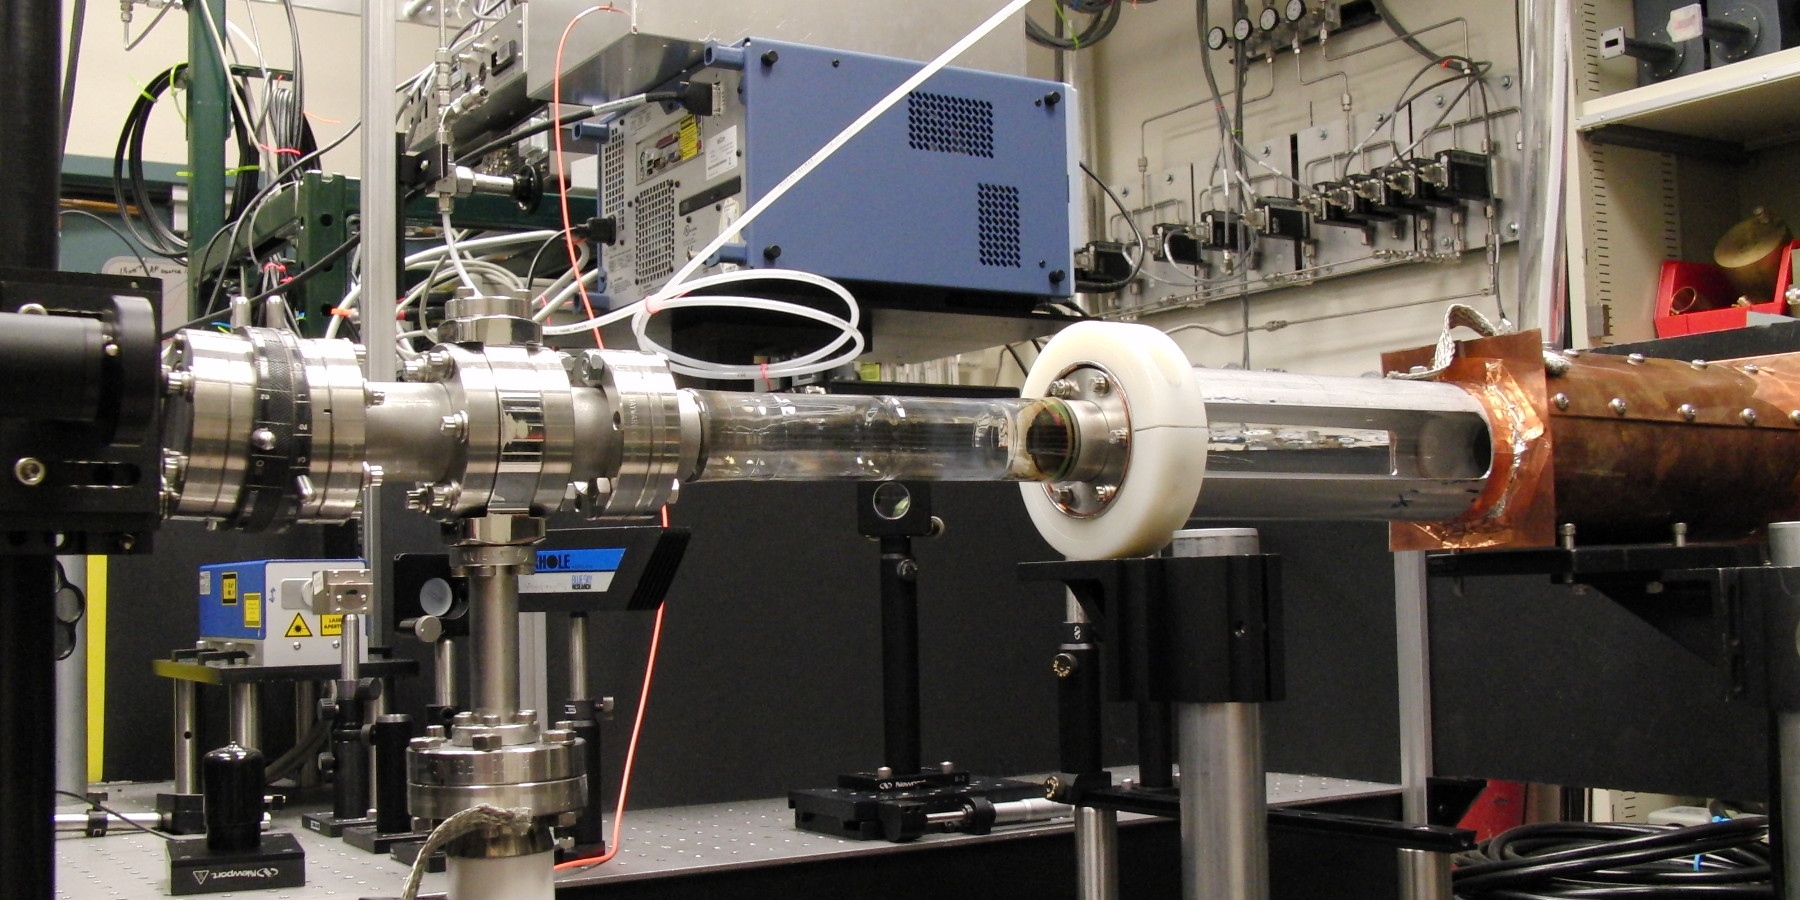
\includegraphics{./chapters/experiment/figures/appphoto.jpg}}
  \caption{Photograph of the discharge apparatus.}
  \label{fig:appphoto}
\end{figure}
The apparatus was supported on an optical breadboard 2.54 cm diameter posts and
angle brackets. Attached to one of the angle brackets was a small optical
breadboard with four bolts which served as physical references for aligning and
positioning the apparatus.

All electrical measurements were made with a LeCroy \smaller{6100A} WaveRunner
oscilloscope which had a bandwidth of 1.0 GHz. Electrical connections to the
oscilloscope were made with the shortest practical lengths of \smaller{RG 50/U}
coaxial cable and terminated at 50 $\Omega$ unless otherwise noted. The voltage
of the pulser was monitored from an internal $1:1000$ divider, and the current
was via a current shunt located in a break of the outer conductor of the
transmission line. The current shunt was composed of 9, low inductance, $1.0
\Omega$ resistors connected in parallel. Figure~\ref{fig:bcs}
\begin{figure}
  \centering
  \setlength\fboxsep{0pt}
  \setlength\fboxrule{1.0pt}
  \fbox{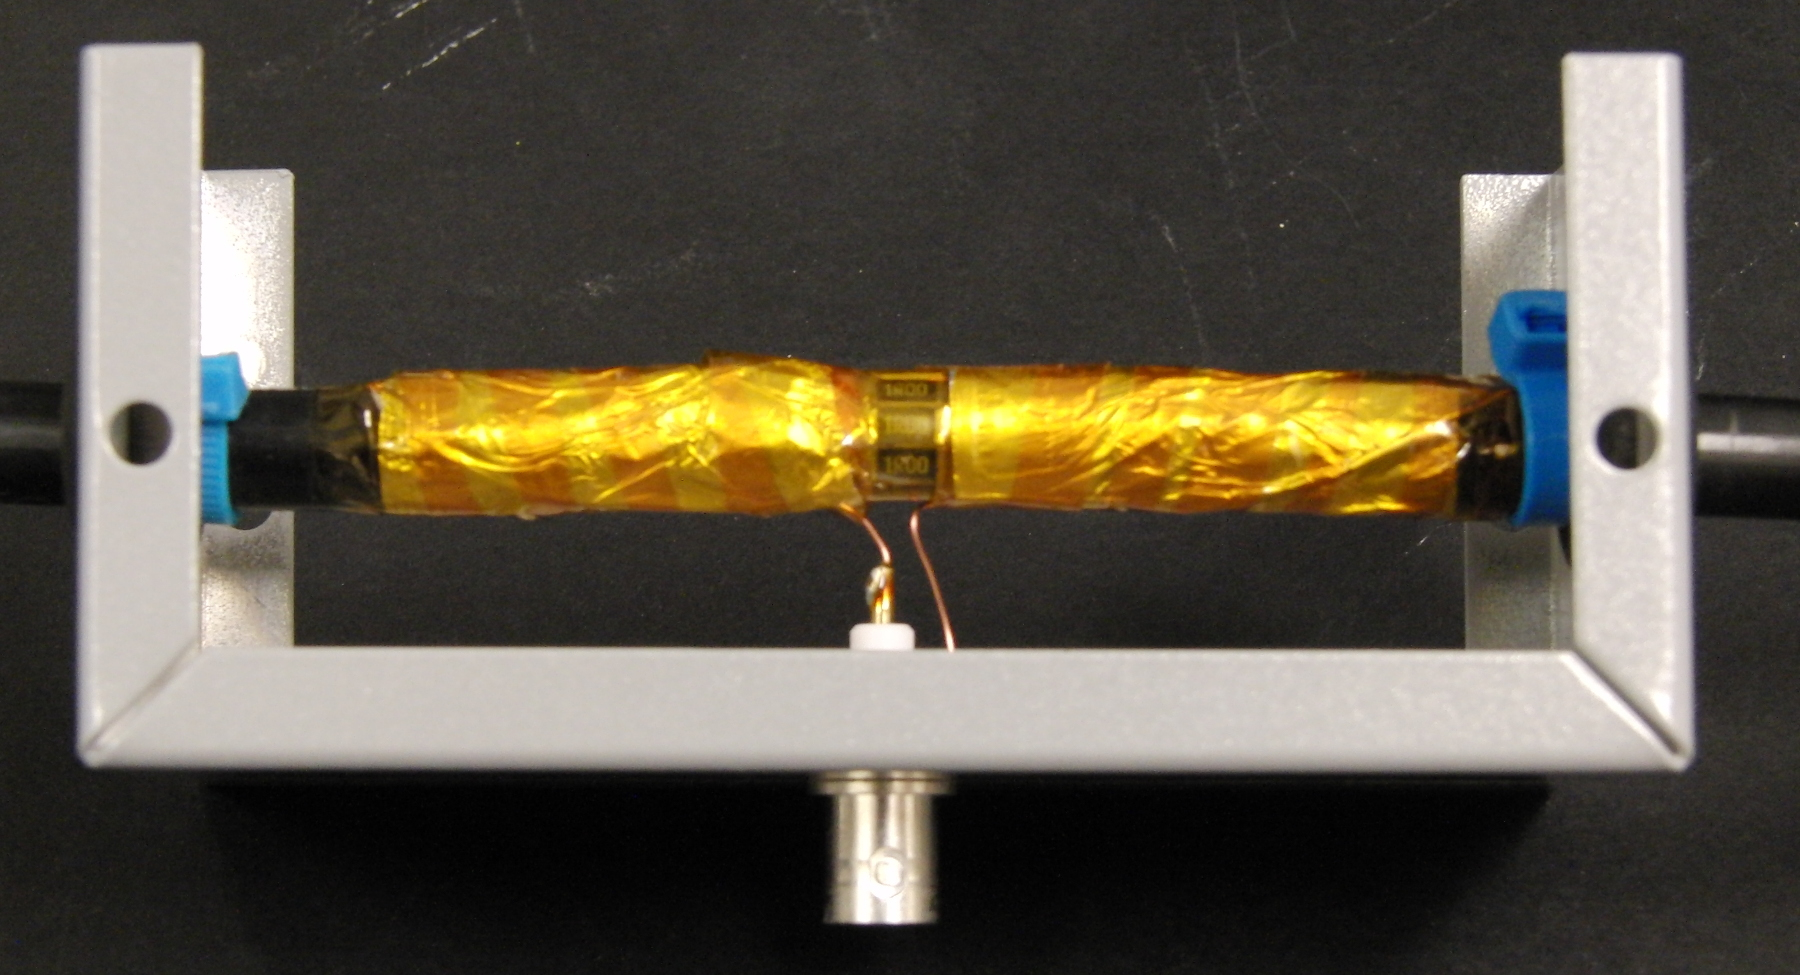
\includegraphics{./chapters/experiment/figures/bcs.jpg}}
  \caption{Photograph of the back-current shunt used to measure the current
  characteristics of the \acs{rpnd}.}
  \label{fig:bcs}
\end{figure}

Data were retrieved from the oscilloscope with a desktop computer via a
\textsc{gpib} connection. A LabView interface was used to interface with the
oscilloscope and additional instruments. Analog inputs and outputs (such as
laser control and pressure sensing) were handled by a \textsc{srs}
\smaller{sr850 dsp} lock-in amplifier which performed as an \emph{ad hoc} data
acquisition system.

\section{Operating Procedure \& Conditions}

At the beginning of each day of operation, the system was first pumped down to
base pressure. After this, the primary pump path was closed in favor of the
needle valve bypasses. The helium flow was then initiated at 25.0 sccm. Then,
the system pressure was adjusted to 3.0 Torr.

Once the pressure reached equilibrium, the pulser was turned on. The plasma was
allowed to run at this condition for one hour in order to remove built up
contamination on the walls and electrodes. During this time, the pressure of the
system would typically drift downwards by several percent. Afterward, the
pressure would be adjusted to the desired operating condition.

It was frequently necessary to turn off the pulser in between experiments. In
these cases, once the pulser was turned on, the plasma was allowed to run for 15
minutes before any measurements were made. This was necessitated by observable
changes in the emissions and current-voltage characteristics during the first 15
minutes of operation. Additional increases to this warm up time resulted in no
appreciable changes to any of the measured data.

Measurements were made for a range of pressures, including: 0.3, 0.5, 1.0, 2.0
3.0, 4.0, 8.0, and 16.0 Torr. The lower limit was set by the pumping speed of
the roughing pump. Difficulty in obtaining reliable plasma breakdown at
pressures above 16.0 Torr set an upper limit on the pressure range. Experimental
measurements of optical properties were obtained at three axial locations: 7.6,
15.2, and 22.9 cm, relative to the anode. These will frequently be referred to
as upstream, midstream, and downstream locations, respectively.

\section{Initial Observations}

Plasma characteristics could be divided into approximately three cases: low,
intermediate, and high pressure. At the low pressures, 0.3, 0.5, and 1.0 Torr,
it was difficult to initiate a discharge. Frequently, the plasma would have to
be started at more moderate pressures, and then adjusted to the desired
condition. At these conditions, the plasma was dim compared to the ambient room
light and a dull purple. It appeared to be well separated from the walls.
Visually, the diameter of the plasma was estimated to be about 2 cm, however
this increased with pressure. Also occurring at these conditions was a large
amount of electronic noise. Nearby instruments, such as the computer mouse, and
lock-in amplifier, would occasionally malfunction at these conditions.

At moderate pressures, 2.0, 3.0, and 4.0 Torr, the plasma expanded radially to
fill the whole of the discharge volume. Compared to ambient conditions the
plasma was bright with an orange-pink hue. Electrical interference disappeared
at these conditions, and the plasma initiation was relatively easy.
Nevertheless, at the beginning of each day several thousand pulses could be
required before a visible plasma was formed. Interestingly, the plasma extended
well past the cathode/ground and to the pumping section (connected to ground at
a separate point). Presumably, this is a result of the relatively small cathode
area compared to the large anode area. The build up of space charge limits the
current extraction from the intended cathode, subsequently the electrode further
downstream begins to contribute.

For the higher operating pressures, 8.0 and 16.0 Torr, the brightness of the
plasma decreased, though not to the level of the low pressure discharge. In
addition, the plasma remained volume-filling. However, it did not visibly
extended past the cathode. Discharge initiation was difficult at these operating
conditions and, as in the low pressure case, the plasma would have to be started
at more amenable conditions. No electrical interference was noted for this
pressure range.

Cursory examination of the voltage signal revealed a large number of reflections
in the system. These can be seen in figure~\ref{fig:waveform},
\begin{figure}
  \centering
  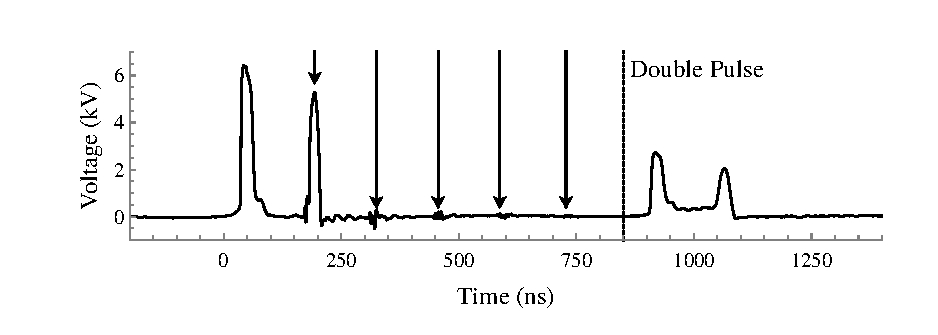
\includegraphics{./chapters/experiment/figures/waveform.eps}
  \caption{Typical voltage waveform of the \acs{rpnd}. Arrows indicate
  reflections back to the pulser. The pulser exhibited a double pulsing
  phenomena, indicated by the dotted line.}
\end{figure}
a typical voltage waveform with overlaid arrows indicating the reflected pulses.
These can be attributed to the impedance discontinuity at the electrode. Also
observable in the waveform is a second pulse and its associated reflection. This
is believed to be a peculiarity of the particular power supply used. The
majority of the presented results, particularly those concerning the fast
dynamics will only consider the initial pulse.

\section{Field Calculations}

The electric field characteristics of the discharge system was analyzed using a
two-dimensional, electrostatic solver, Ansoft Maxwell 9. Figure~\ref{fig:fields}
\begin{figure}
  \centering
  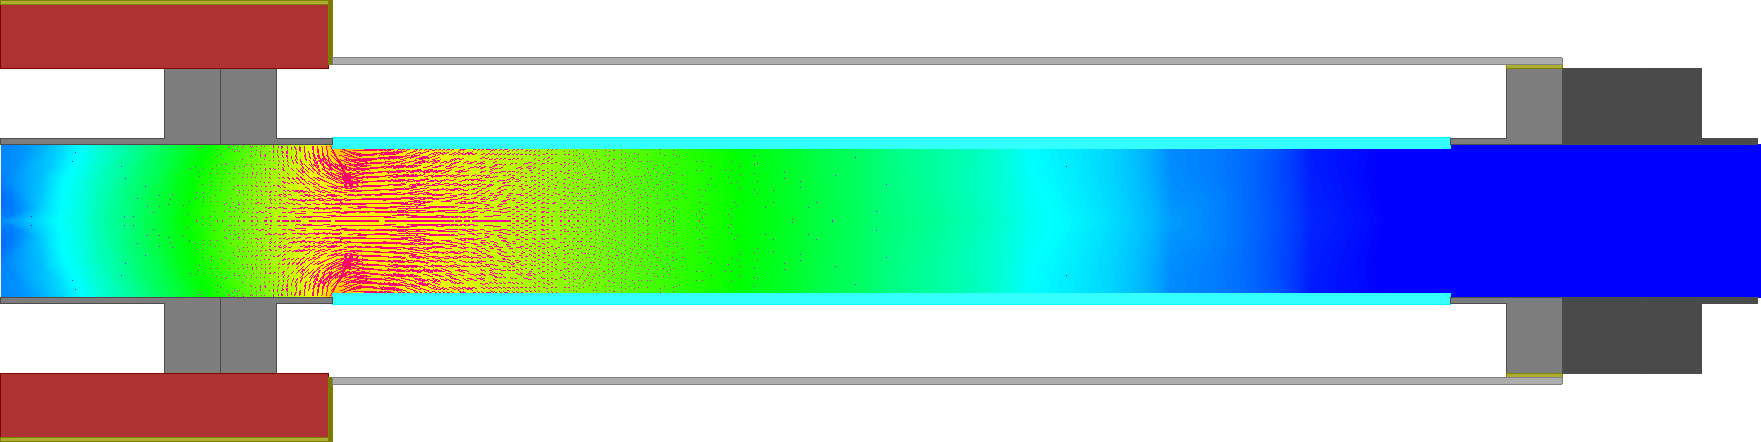
\includegraphics{./chapters/experiment/figures/fields.jpg}
  \caption{Heat map and vector plot of the electric field in the \acs{rpnd}
  discharge apparatus.}
  \label{fig:fields}
\end{figure}
is a logarithmic heat map of the electric field magnitude, with overlaid
electric field vectors (in magenta). The electric field varies significantly
over the length of the discharge apparatus, with a peak near the axial location
of the glass tube followed by a monotonic decline. These characteristics are a
large departure from simple case of two parallel electrodes in which the field
is uniform throughout. This can be attributed to the presence of the external
ground shield. Though this does complicate the field characteristics, the
proximity of the ground results in a much higher electric field than would
otherwise be achievable.

While the off-axis field lines all feature notable radial components,
particularly close to the anode the center line does not.
Figure~\ref{fig:centere}
\begin{figure}
  \centering
  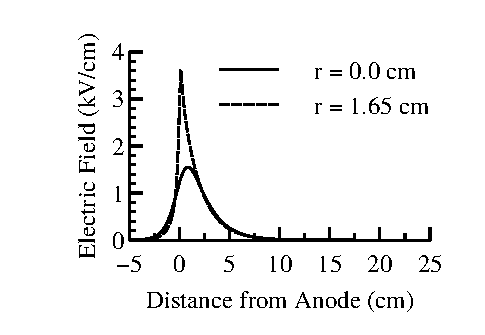
\includegraphics{./chapters/experiment/figures/centere.eps}
  \caption{The magnitude of the electric field along the center and outside of
  the discharge apparatus.}
  \label{fig:centere}
\end{figure}
is a plot of the magnitude of the electric field along the central axis of the
discharge apparatus and the outside, adjacent to the glass tube. The location of
the anode is defined as the location of the glass-to-metal seal.

\section{Energy Coupling}



\section{Absorption Setup}
The \acs{las} setup was based upon the used of a distributed-feedback
laser diode. Temperature and current control of the diode provided
coarse and fine tuning, respectively, for the output frequency. It was
found that it was unnecessary to adjust the temperature for the diode
once the correct transition was found, therefore all tuning was
accomplished using current tuning.

The laser diode was produced by Toptica Photonics (model
\#LD-1083-0070-DFB-1), and had a nominal operating power of 70 mW at a
center wavelength of 1083 nm. The diode was held inside a Toptica DL-100
diode housing which contained an integral thermoelectric cooler and
collimating optics. The operation of the diode was controlled by a
Toptica DC 110 monitor, DCC 110 current control, DTC 110 temperature
control, and SC 110 scan control.

A schematic of the optical layout for the absorption experiment can be
seen in Figure \ref{fig:abslayout}. Immediately after exiting the
housing, the beam was passed through an optical isolator in order to
prevent instabilities from back reflections. Next the beam was
attenuated using a neutral density filter in order to keep its intensity
below the saturation level for the transition. Following that, the beam
passed through two apertures for alignment. Here, the beam was split by
a partially reflecting mirror. Approximately 98\% of the beam was
allowed to pass through to a reference photodiode (Thorlabs DET300).
After passing through the plasma, entered another aperture to limit
near-coincident plasma emissions. The background emissions were further
reduced using a long pass filter with a cutoff of 1000 nm. Finally, the
beam was coupled into an optical fiber which connected to the detection
electronics.

The transmitted laser light was detected with an InGaAs photodiode
(Thorlabs DET410). The signal from the diode was often too small to
detect, so the output of the signal photodiode was sent through a
voltage amplifier (Femto HVA-200M-40-B). The light response of this
system is limited by the photodiode which has a nominal rise time of
five nanoseconds. The signal from the amplifier was terminated by a 50
ohm terminator and sensed by the aforementioned oscilloscope.

\subsection{Acquisition Process} The actual acquisition process required
a specific series of steps in order to properly account for all noise
sources. In order to accommodate this process, a custom LabView script
was used to automate the acquisition of the laser transmission spectra.
Generally speaking, the signal can be described as
\begin{equation}
  V_\mathrm{total} = V_\mathrm{signal} + V_\mathrm{background} +
                     V_\mathrm{plasma}.
\end{equation}
In order to remove the background signal, the acquisition scr

\section{Emissions Setup}


  \chapter{Metastable Measurements}\label{chp:metastables}
    As was noted in chapter~\ref{chp:introduction}, measurements of the \acs{rpnd}
been mostly limited to the afterglow plasma or time-integrated quantites.
Electric field measurements, either with capacitive probes or nonlinear
wave-mixing, thus far provide the only detail of the \acs{rpnd} during its
development. Though the electric field can be used to estimate electron
densities and reaction rates in the plasma, this requires a number of additional
assumptions.

As a result, there is a lack of reliable information on the particle properties
of the \acs{rpnd} during its development. That said, such information is
essential to confirming the present understanding of how these discharges
develop, optimizing them for specific applications, and providing important
benchmarks for numerical simulations. Therefore, a clear need exists for direct
measurements of the \acs{rpnd} particle properties.

Unfortunately, these measurements present a significant challenge for most
traditional plasma diagnostics. In most situations, the obvious choice would be
the Langmuir probe for its simplicity and ease of implementation. However, the
fast variations in the plasma potential, slow response of the ion, and high
collisionality all preclude this approach \cite{Lieberman2005}. Furthermore, any
physical probe would act as a significant perturbation in the system.

The logical alternative to physical probes is the use of optical diagnostics,
however these have their own associated difficulties. Electrons cannot be
studied by their emissions because, with the exception of bremsstrahlung, they
do not emit light. This leaves the light emitted from excited atoms. Atomic
emission spectroscopy can be used to measure many different plasma quantities,
from electron density, to local electric field strength. Unfortunately,
spontaneous emission can be a slow process compared to the development of the
\acs{rpnd}. For example, the fastest neutral helium transition in visible
wavelengths (3$^3$D$_3$-2$^3$P$_2^\cdot$) has a radiative life of 14 ns
\cite{Ralchenko2011}.

This suggests that instead of waiting for spontaneous emission to occur, it may
be better to use some form of active spectroscopy. Though the added complexity
of a well-characterized light source is undesirable, it adds several interesting
possibilities. For example, Thomson scattering provides a means for direct
interaction with electrons. In addition, it has a high spatial and temporal
resolution and is able to measure the electron density and temperature
simultaneously \cite{VanGessel2012}. However, the electron density limit of
$5\times10^{12}$ cm$^{-3}$ is too low for use with the \acs{rpnd} which may have
electron densities well below this \cite{Pai2009}.

With the ability to directly interact with electrons, the next alternative is to
target one of the excited states of helium. The lowest such state, the triplet
metastable (2$^3$S), resides at 19.82 eV. This is a relatively large energy gap
for an atom and indicates that virtually no such states should exist at room
temperature. The triplet metastable (and all higher-energy states in helium)
will be populated exclusively by energetic electrons. Therefore, a measurement
of the triplet metastable level is a useful indicator of the degree of helium
excitation as the \acs{rpnd} develops, and could potentially be used to infer
some properties of the electron population.

Perhaps the most straightforward approach to a measurement of the triplet
metastable density is with absorption spectroscopy. This approach has a long
history in the study of metastables in gas discharges, going back at least six
decades \cite{Phelps1953}. At its most basic, the technique involves
illuminating a plasma with light matching a transition between the metastable,
and some upper level and measuring the amount of light transmitted. The amount
of light transmitted is proportional to the metastable density integrated along
the path of the light traversing the plasma. The bandwidth of this measurement
is only limited by the time required for the light to pass through the plasma.

\section{Setup}

Traditionally, the light used in absorption spectroscopy has been supplied by
discharge tubes with the same gas as the system under study. Though
straightforward, this approach is limited by the luminosity of the discharge
tube, and the fact that the emitted radiation is isotropic. More recently,
Millard et al. noted that diode lasers provide a greatly improved light source
that provides simple spatial selectivity, at intensities which can easily exceed
the saturation limit \cite{Millard1998}.

As with the study by Millard et al., the decision was made to study the
transition from the triplet metastable to the 2$^3$P$^\mathrm{o}_{0,1,2}$ (at
approximately 1083 nm). This was done for several reasons. For one, the closest
helium transition is over 7 nm away, making it relatively isolated. In addition,
the different levels or values of $J$ are all within the tuning range of a
single diode. As each level has a different degeneracy, $g$, the strength of
absorption varies depending on the selected level. Thus, the absorption strength
can be increased for low densities, or decreased at high densities, improving
the dynamic range of the diagnostic.

The laser used was a distribute feedback laser diode, produced by Toptica, model
LD-1083-0070-DFB-1. The specified linewidth of the laser was 3 MHz, well below
the natural linewidth of the transition, 10.2 MHz. This situation can be
exploited to directly measure the gas temperature of the system, as will be seen
in the next section. The diode was rated for a total output power of 70 mW, with
a beam size of 1 mm by 3 mm and a vertical polarization. The diode was housed in
a Toptica DL DFB housing which incorporated the collimating optics. A Toptica
DCC 110 was used to provide current control for the diode laser, and a Toptica
DTC 110 was used to control the thermoelectric cooler for the diode.

The layout in figure~\ref{fig:laser}
\begin{figure}
  \centering
  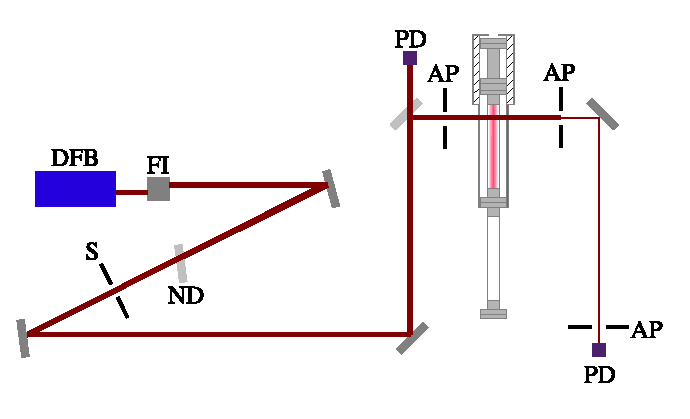
\includegraphics{./chapters/metastables/figures/laser.eps}
  \caption{Optical beam path of the laser in the absorption spectroscopy
  experiment. DFB - Distributed feedback laser diode; FI - Faraday isolator; ND -
  neutral density filter; S - shutter; PD - photodiode; AP - aperture.}
  \label{fig:laser}
\end{figure}
reflects the optical beam path used in the absorption experiment. The laser
light is produced by the distributed feedback laser diode (DFB). It then enters
a Electro-Optics Technology, Inc. Faraday isolator (FI) which prevents
back-reflections from entering the diode. Without the isolator in place, such
back-reflections can cause mode-hopping, resulting in unreliable tuning. The
laser intensity is then reduced by a neutral density filter (ND). Afterward, the
laser passes through a Vincent Associates electronic shutter (S). Then, the beam
is split by a Thorlabs BSF10-C beam sampler at a 45$^\circ$ angle. This reduced
the laser intensity below the saturation intensity (0.45 mW/cm$^2$) of the
transition. Collimation to a 1 mm circle, and alignment were provided by two
apertures (AP) on both sides of the discharge apparatus. The beam exiting the
apparatus was then sent through a final aperture to spatially filter plasma
emissions before being a Thorlabs F240SMA-780 collimation package was used to
couple the light into an optical fiber.

Behind the beam sampler was a Thorlabs DET300 germanium photodiode. The signal
from this photodiode was terminated at 1 M$\Omega$ and used to monitor the beam.
The opposite end of the optical fiber was affixed to a Thorlabs DET410 InGaAs
photodiode. The photodiode signal was amplified by a Femto HVA-200M-40-B voltage
amplifier before being sent to the oscilloscope. The time resolution of the
metastable measurements was determined by the InGaAs photodiode which had a
specified rise time of 5 ns.

In order to measure the absorption of the laser, it was first necessary to tune
the laser to the correct wavelength. This matter was complicated by the lack of
a wavemeter with sufficient precision and accuracy. As a result, a signal
generator was used to sweep the laser current so as to cover a frequency range
of 40 GHz. The temperature of the diode was then slowly adjusted until
absorption peaks corresponding to the 2$^3$S$_1$-2$^3$P$_{0,1,2}^\mathrm{o}$
transition were observed. The conversion between diode and wavelength was
measured with a CVI Melles Griot ET-25.4-10.00-30, solid dielectric etalon. It
was found that a temperature of 36$^\circ$ C and a current of 63 mA produced
resulted in an output wavelength of approximately 1082.9 nm.

As described in chapter~\ref{chp:experiment}, data acquisition was handled by a
LabView program, connected to the oscilloscope by GPIB\@. The auxiliary outputs of
the SRS SR850 lock-in amplifier were used to adjust the diode laser current (via
the DCC 110 module), and to trigger the electronic shutter. One of the auxiliary
inputs of the lock-in amplifier was used to read out the pressure from the
pressure controller.

Data were acquired for a range of pressure 0.3-16.0 Torr, and at three axial
locations: 5.08, 12.7, and 20.32 cm, relative to the glass-metal seal of the
anode. In reference to their location relative to the gas inlet these will be
referred to as the `upstream', `midstream', and `downstream' locations,
respectively. For each combination of location and pressure, absorption spectra
were measured over $\pm3.85$ GHz relative to the nominal transition frequency of
the 2$^3$S$_1$-2$^3$P$_0^\mathrm{o}$ transition at intervals of 154 MHz. The
absorption spectra were measured for time domains of $-300$-$1700$ ns relative
to the voltage pulse. Additional measurements were made at the midstream
position of the metastable densities from $-88$-$712$ $\mu$s in order to
investigate the loss mechanisms of the metastables.

The broadband electronic noise emitted by the fast pulses was a persistent issue
and presented one the greatest challenges to measurements during the \acs{rpnd}
development. As described above, the InGaAs photodiode was removed from the
immediate area surrounding the discharge by an optical fiber. The optical fiber
was routed through a small opening in a grounded metal box where both the
photodiode and the voltage amplifier resided. In addition, the DC power supply
of the voltage amplifier was connected to an outlet on a Tripp-lite Isobar
intended to provide additional isolation. The photodiode was connected directly
to the input terminal of the amplifier, while the amplifier was connected to a
BNC bulkhead adapter by a 10 cm length of RG 50/U. The final connection to the
oscilloscope was made by an additional 10 cm length of RG 50/U, running from the
BNC bulkhead connection.

Figure~\ref{fig:transmitted}
\begin{figure}
  \centering
  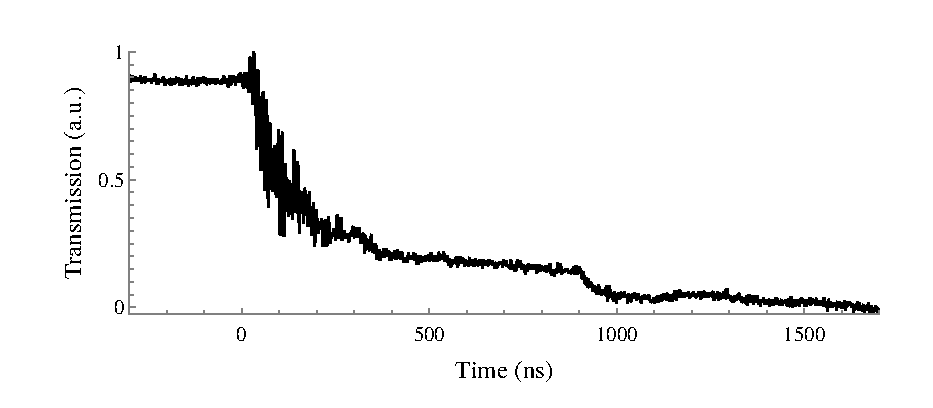
\includegraphics{./chapters/metastables/figures/transmitted.eps}
  \caption{Measurement of the transmitted laser light at the nominal transition
  wavelength at 4.0 Torr of helium.}
  \label{fig:transmitted}
\end{figure}
shows the transmission signal measured at the nominal transition wavelength for
a \acs{rpnd} in 4.0 Torr of helium. The signal is the average of 200 independent
pulses, further sampling had no appreciable effect on the waveform. As can be
seen, despite the efforts to limit the electrical interference, there is still a
substantial amount of noise present in the transmission signal. This is most
noticeable in the large ringing which occurs for the first 200 ns after the
voltage pulse. Without any kind of compensation, it would be impossible to
obtain reliable measurements of the transmission signal

\section{Absorption Analysis}

The noise produced by the \acs{rpnd} was relatively consistent between pulses
and over the duration of each experiment. As a result, it was possible to
correct for the electrical noise, as well as any spontaneous plasma emissions,
by measuring the signal from the photodiode in the absence of the laser. The
acquisition process proceeded as follows:
\begin{enumerate}
  \item Set desired laser wavelength.
  \item Wait 5 s for laser output to settle.
  \item Acquire 200 waveforms from photodiode.
  \item Close shutter.
  \item Acquire 200 waveforms from photodiode.
  \item Repeat
\end{enumerate}
The second set of waveforms was then subtracted from the first in the
post-processing stage. The effect of this subtraction can be seen in
figure~\ref{fig:contours}
\begin{figure}
  \centering
  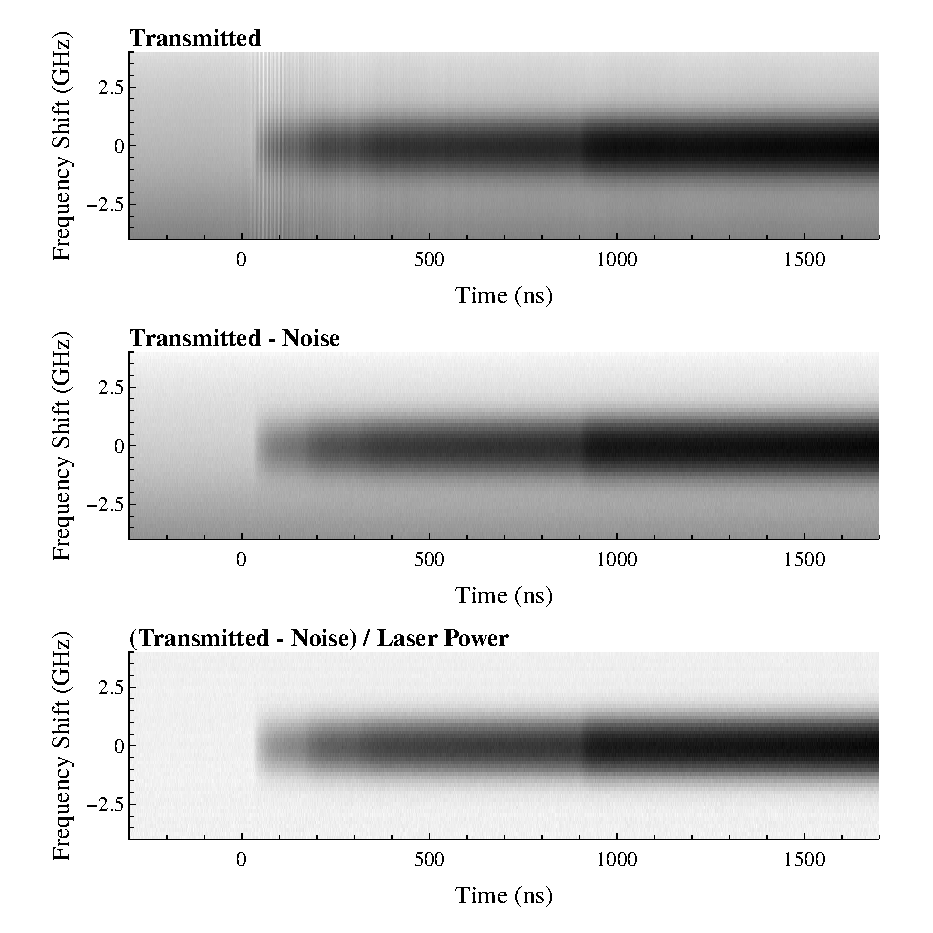
\includegraphics{./chapters/metastables/figures/contours.eps}
  \caption{Heatmaps of the transmitted laser signal for the 4.0 Torr condition at 
  various stages of post-processing.}
  \label{fig:contours}
\end{figure}
where the top heatmap shows the initial set of acquisitions with the laser on,
and the middle heatmap shows the transmitted signal with the noise subtracted.

As the laser diode current was changed in order to scan the wavelength across
the transition, the output power also changed by a small but significant amount.
The produces the gradient-like appearance of the top two plots in
figure~\ref{fig:contours}. In order to obtain a measurement of the unattenuated
laser power, the above acquisition procedure was repeated with the plasma off
for each operating condition. This made it possible to correct for the varying
laser power and to produce properly scaled transmission spectra.

These transmission spectra were then analyzed using a transmission model based
on the absorption cross sections described in chapter~\ref{chp:theory}. In a
one-dimensional system, the change in intensity of an incident photon field
(below the saturation limit), can be expressed as
\begin{equation}
  \frac{dI(x, \omega)}{dx} = -\sigma(\omega) N(x) I(x, \omega)
\end{equation}
where $I$ is the intensity of the photon field as a function of distance $x$,
$\omega$ is the frequency of the photons, $N$ is the density of the interacting
species, and $\sigma$ is the interaction cross section. This equation has the
simple solution,
\begin{equation}
  T(\omega) = \frac{I(x, \omega)}{I_0(\omega)}
            = \exp\left[-\sigma(\omega) \int_0^x N(x') dx'\right],
  \label{eq:transmitted}
\end{equation}
where $T$ is the transmitted intensity fraction, and $I_0$ is the initial
intensity of the photon field. The absorption can be trivially obtained from the
equation $A(\omega) = 1 - T(\omega)$.

For the purpose of analyzing the absorption, a quantity called the
line-integrated density will be defined. This is simply, $\nint = \int_0^x
N(x')dx'$. Equation~\ref{eq:absorb} can be used to determine the absorption
cross section. However, this requires that a lineshape be specified. If
possible, it is preferable to select either a purely Gaussian or purely
Lorentzian lineshape as the Voigt profile (equation~\ref{eq:voigt}) is
accompanied by a significantly larger computational cost. This can be determined
by a comparison of the relative widths of the different broadening mechanisms.
For a temperature of 300 K and a pressure of 8.0 Torr, it is found that $\dwd =
1.7$ GHz and $\dwa = 0.21$ GHz. Because neither broadening mechanism is
significantly dominant, the choice was made to analyze the data with a Voigt
profile, despite the added computational cost.

Equations~\ref{eq:transmitted},~\ref{eq:absorb}, and~\ref{eq:voigt} can be
combined to form a model equation for the transmitted spectrum. It can be seen
that only two unknowns exist: the gas temperature, $T_g$, and the
line-integrated density, $\nint$. For each time step, this model equation was
matched to the measured spectrum using the Levenburg-Marquardt algorithm
\cite{Marquardt1963} as implemented by the SciPy library \cite{Jones2001}.
During the matching process, it was observed that the diode current for which
absorption was optimized would shift over time. This was assumed to be the
result of small, long-term variations in the diode temperature that were not
adequately compensated for by the temperature control system. This corresponded
to a frequency drift of $\pm60$ MHz between experiments. For each experiment,
this frequency offset was measured for the spectrum with the largest absorption
signal and was then used to correct the analysis of all other spectra.

\section{Results}

The matching algorithm proved robust enough to automatically match the
transmission spectrum at each time step with no user intervention.
Figure~\ref{fig:matching}
\begin{figure}
  \centering
  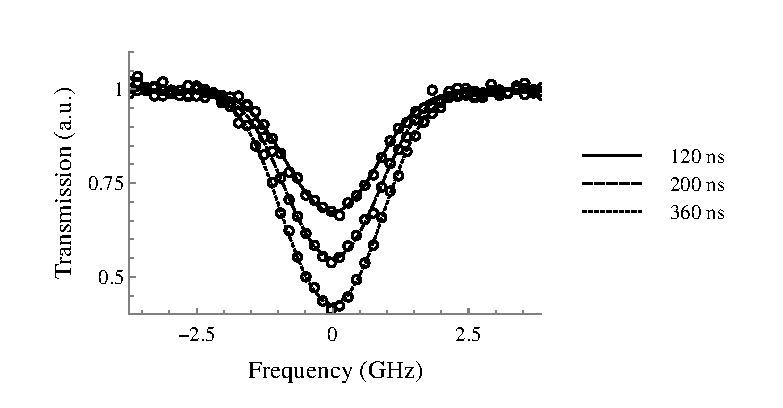
\includegraphics{./chapters/metastables/figures/matching.eps}
  \caption{Comparison of the measured transmission profile (open symbols) and
  the computer-generated matches for at several different times for the 4.0 Torr
  operating condition.}
  \label{fig:matching}
\end{figure}
shows three examples of the measured transmission spectra along with the
computer-generated matches. The measure data far from the peak coincide almost
perfectly with an unabsorbed signal. In addition, the spectrum at 120 ns shows
no evidence of the noise caused by the discharge. The variation in the baseline
transmission signal is approximately 0.02. This sets a minimum line-integrated
detection limit of approximately $3.0 \times 10^{14}$ m$^{-2}$, though the
actual value will depend to some extent on the pressure and temperature.

\subsection{Temperatures}

The temperatures calculated for the metastables from the laser-absorption
spectroscopy are shown in figure~\ref{fig:temperatures}.
\begin{figure}
  \centering
  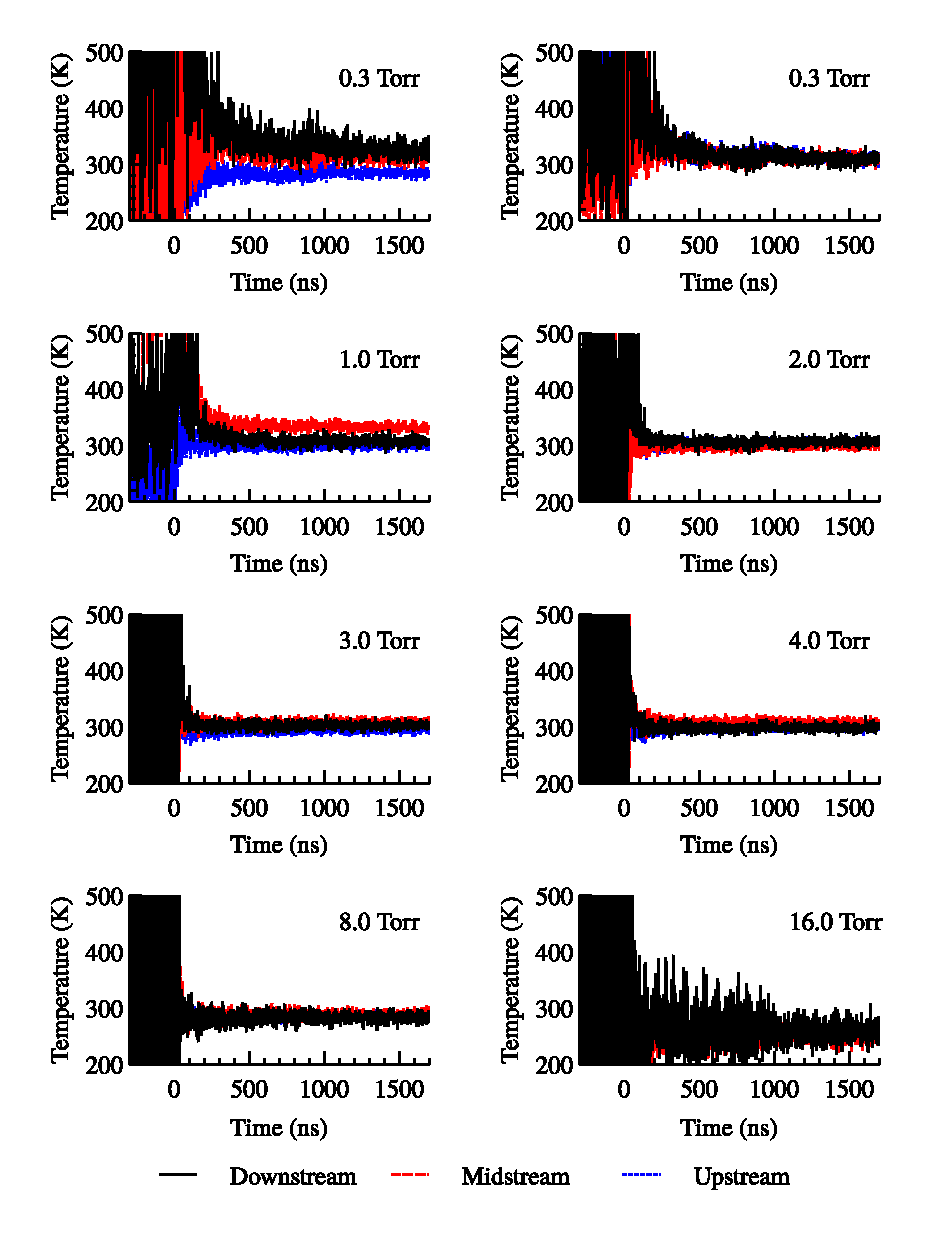
\includegraphics{./chapters/metastables/figures/temperatures.eps}
  \caption{Plot of the gas temperatures at each of the operating
  pressures and each axial location as a function of time.}
  \label{fig:temperatures}
\end{figure}
Prior to the pulse, the temperature estimates are subject to large variations.
This is a result of the low metastable densities which precede the pulse.
Without a substantial metastable population to work with the matching algorithm
has difficult discriminating between a combination of low temperatures and low
densities (a small narrow absorption spectrum) versus high temperatures and high
densities (a very broad absorption spectrum).

It is not possible to precisely calculate the error for the matching process at
each time step, however it is possible to estimate the standard deviation. In
all cases, the estimated standard deviation is less than 10 K by the end of the
measurement period. Based on the covariance estimates, there appear to be no
meaningful trends over the measurement period or between measurement locations.

In order to more clearly compare the temperatures at the different operating
conditions, the results for each location were combined and averaged over the
final 200 ns. This was then plotted with respect to the energy deposition
calculations from chapter~\ref{chp:experiment}, divided by the gas density.
The results are shown in figure~\ref{fig:tvp}.
\begin{figure}
  \centering
  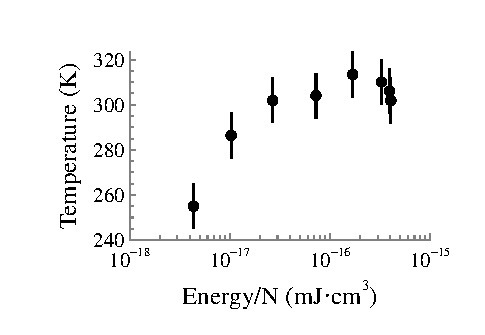
\includegraphics{./chapters/metastables/figures/tvp.eps}
  \caption{Plot of the average gas temperature as a function of deposited
  energy.}
  \label{fig:tvp}
\end{figure}
For the majority of operating conditions, there is little to know statistical
difference between the results and room temperature. The one exceptional
condition is the 16.0 Torr operating condition at 4.33$\times10^{-18}$
mJ/cm$^3$ with a mean temperature of 255 K. As the glass of the discharge tube
as at room temperature for all experimental conditions, this does not appear to
be a reasonable result for the temperature. Examination of the individual
absorption spectra did not reveal any obvious errors in the calculated matches.
However, as will be seen later, the metastables were the least dense at 16.0
Torr. This, coupled with the large variation of the temperatures in
figure~\ref{fig:temperatures} suggest that the standard deviation is potentially
lager than 10 K. Such a situation would explain the unreasonable temperature
obtained for this condition.

The literature provides only a limited number of direct temperature measurements
for similar systems. The most similar work in appears to be that of Walsh et al.
\cite{Walsh2010} in which the temperature of a \acs{rpnd} in helium with a small
admixture of oxygen was measured by optical emissions. The geometry consisted of
two cylindrical steel electrodes separated by 2 mm with a single dielectric
barrier between the two, a gas flow rate of 5 slm, at atmospheric pressure.
Temperatures ranged from 300-340 K, depending on the average power dissipated in
the plasma. Walsh et al. suggest that the observed temperature increase is a
result of Joule heating, that is, heating of the gas as a result of electrons
colliding with neutral particles. As the neutral collision frequency scales
linearly with pressure, this would certainly explain the negligible heating
observed in figure~\ref{fig:tvp}. The presence of a large fraction of a
molecular gas (oxygen) presents another potential heating mechanism when
dissociation occurs, called Franck-Condon heating, and excitation of rotational
and vibrational states which relax to translational energy
\cite{Kiehlbauch2003}.

Other experiments have demonstrated minimal gas heating, as in the case of
plasma bullets \cite{Laroussi2005, Lu2006}, while others have measured final
temperatures ranging from 400-1000 K \cite{Pai2009, Popov2011, Zuzeek2010} (see
appendix~\ref{chp:oes} for detailed study in air). From the available
literature, measurable heating only appeared to coincide with measurements of
\acs{rpnd}s in molecular gases. This emphasizes the importance of the heating
mechanisms mentioned earlier and likely plays a large role in the nonthermal
nature of the atmospheric pressure helium plasmas.

Recent simulations and rate calculations \cite{Takashima2011, Aleksandrov2007}
have provided estimates of the electron temperature in the range of 10-20 eV. As
a result, all of the discharges mentioned are very much nonthermal in nature.
That said, the negligible heating in the helium \acs{rpnd} studied here presents
a significant advantage for many applications, as even the moderate temperature
increases in molecular discharges can threaten material integrity. For example,
most commercial polymers are only rated to 300$^\circ$ C, making them
susceptible to damage without careful thermal management.

\subsection{Line-integrated Densities}

As described in the analysis section, the laser-absorption spectroscopy also
yielded the line-integrated metastable densities. Figure~\ref{fig:metastables}
\begin{figure}
  \centering
  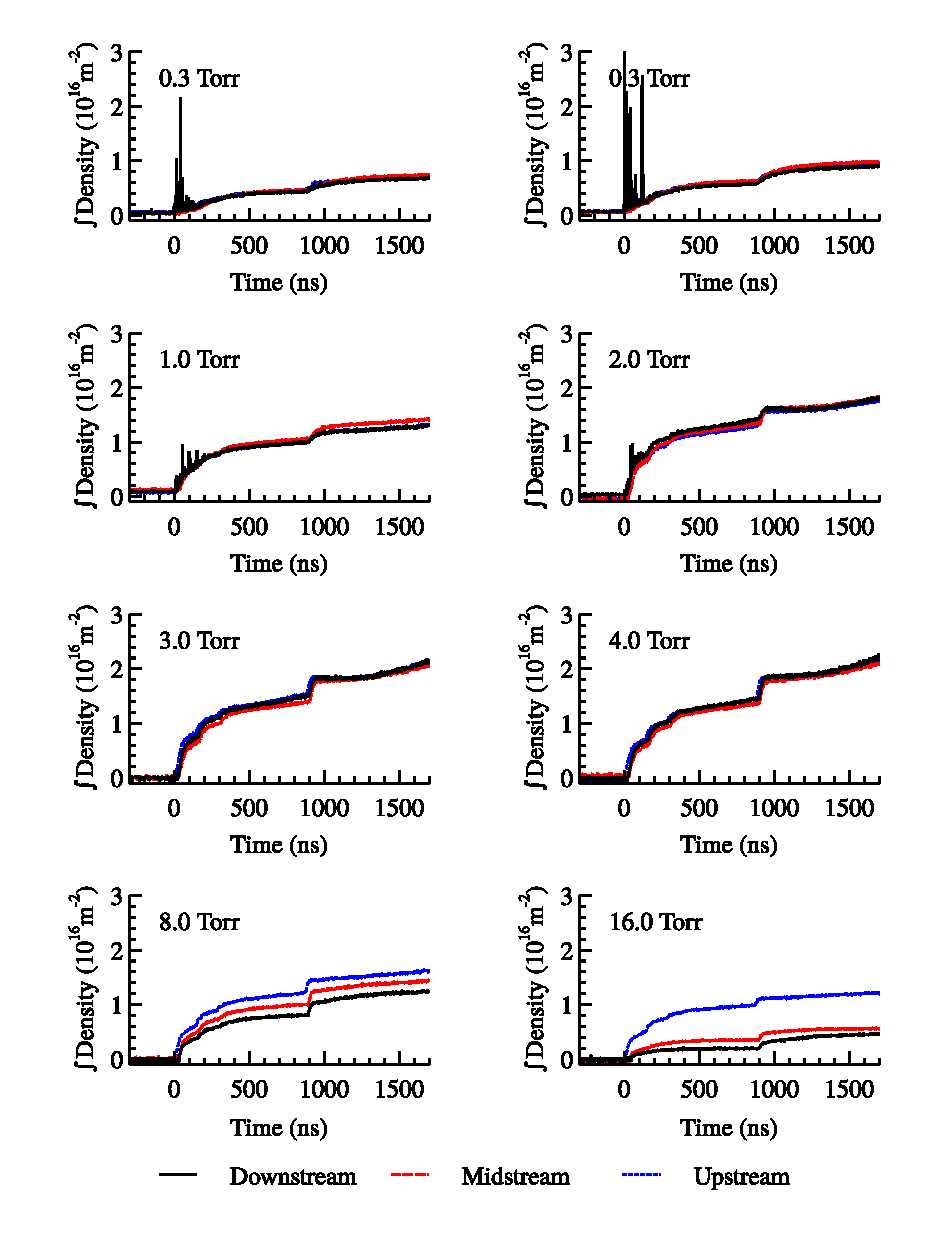
\includegraphics{./chapters/metastables/figures/metastables.eps}
  \caption{Plots of the line-integrated metastable densities at each of
  the operating pressures and each axial location as a function of
  time.}
  \label{fig:metastables}
\end{figure}
features the metastables dynamics for each operating pressure and at each
location. Similar to the temperature measurements, there is a substantial
uncertainty during the pre-pulse period for pressures greater than 1.0 Torr.
However, for 1.0 Torr and below, there are detectable populations of triplet
metastables, around $7\times10^{14}$ m$^{-2}$. These excited atoms are the
remnants of the previous pulses which have not been destroyed. Despite the
efforts made to limit the noise in the signals, there is a significant number of
erroneous data points at pressures below 3.0 Torr in the downstream
measurements. The reason for this is not apparent. The only change was the
position of the mirror directing the transmitted laser light into the fiber
coupler. That is, the position of the photodiode did not change between
measurements. 

The population of the metastable states exhibits several small bursts, in short
succession, after the pulse at about 140 and 270 ns. The timing of these rapid
rises in density correlate to the arrival of pulse reflections. This suggests
that the even after the plasma has formed, additional pulses are still able to
deposit a significant amount of energy in the plasma. In all reported cases, the
final metastable density grew to exceed twice the density after the first pulse.
This appears to contradict the predictions made by the one-dimensional drift
models of Adamovich et al. \cite{Adamovich2009} and Nikandrov et al.
\cite{Nikandrov2008} which stated that little energy is coupled into the plasma
after breakdown occurs. In addition to the smaller bursts in density, another
can be noted at about 900 ns which corresponds to the double-pulsing observed in
the current-voltage characteristics of chapter~\ref{chp:experiment}.

By 200 ns after the pulse, the estimated standard deviation in all cases is
approximately $2\times10^{14}$ m$^{-2}$. Based on this, it can be concluded that
the metastable populations had no significant axial dependence below 8.0 Torr.
However, both 8.0 and 16.0 Torr conditions showed notable differences in the
metastable population as a function of distance from the anode. As might be
expected, the upstream location (closest to the anode) has a high metastable
population than the other two. At 16.0 Torr, the line-integrated density at 16.0
Torr was over twice that of either location.

This behavior is reminiscent of that observed by Vasilyak et al.
\cite{Vasilyak1994} in \acs{fiw} devices. It was noted that the electric field
of the wave would attenuate with distance. In order to interpret this, they
considered the wave to consist of two components: a moving ionization front with
a finite width, and the plasma left in its wake. They state that the plasma,
with its finite conductivity, will have some voltage drop across it, and as it
grows, this drop increases. As a results the voltage drop across the ionization
front can never be greater than the overall potential applied to the system and
is constantly diminishing as it moves away from the energized electrode. If
true, this behavior would be associated with a reduction in the rate of
metastable generation in the front, thus explaining the high pressure data in
figure~\ref{fig:metastables}.

\subsection{Metastable Destruction}

In addition to the fast metastable dynamics, measurements were made of the
long-term trends in metastable population. As previously mentioned, afterglow
measurements such as these are less subject to the noise and bandwidth
limitations of the short timescale measurements. Additionally, without the
applied electric field the compelling nonequilibrium dynamics of the system will
rapidly disappear. Therefore, these measurements do not provide much insight on
the development of the \acs{rpnd}.

However, a large body of work has been conducted on helium afterglow discharges,
making this regime attractive as a point of comparison. In addition, these
measurements capture the peak metastable population which is missing from
figure~\ref{fig:metastables}. As seen in figure~\ref{grotrian}, all excited
states in the triplet manifold will eventually decay to the triplet metastable
level. At 19.6 eV above the ground state, this large metastable population
provides a long-lived energy source that can produced charged particles through
Penning ionization well after the voltage pulse. Therefore, it is important to
understand the full dynamics of the metastable atoms as they play a role in
establishing stable \acs{rpnd}s.

The trends in figure~\ref{fig:long}Additionally, each
\begin{figure}
  \centering
  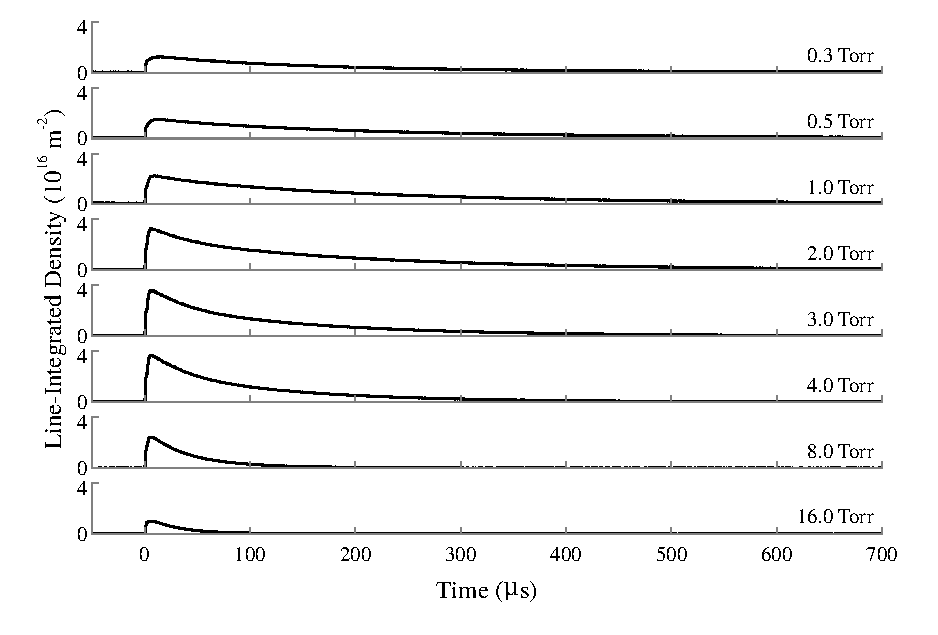
\includegraphics{./chapter/metastables/figures/long.eps}
  \caption{Measurements of the long-duration metastable density trends.
  Exponential fits are indicated by the dotted lines.}
  \label{fig:long}
\end{figure}
show the evolution of the metastables over time for each operating condition.


The long term metastable trends were measured for each pressure at the midstream
location


\subsection{Radial Density Maps}



With the exception of the data from the downstream location at low pressures,
these results are among the first direct measurements of \acs{rpnd} properties
on timescales relevant to its formation. The final temporal resolution was
determined by the photodiode, with a rise time of approximately 5 ns. 

  
  \chapter{Modeling}\label{chp:modeling}
    Though the line-integrated metastable densities are one of only a few
measurements made in the development of the \acs{rpnd}, they only provide a
limited view of what is happening. In addition to the metastables are ions,
electrons, a vast array of other excited states, and the electric fields. In an
effort to expand on the details of what is occurring within the \acs{rpnd}, it
is desirable to develop a model which can infer other properties from the
metastable measurements. This is possible, because the electrons which gain
energy from the electric fields are responsible for the excitation of the
metastables, other atomic states, and ions. The ideal model would solve the
Boltzmann equation (equation~\ref{eq:boltzmann}) for each species, over the
entire geometry, in all dimensions, for as long as was required to reach
equilibrium.

Unfortunately, these requirements are somewhat problematic. Solutions to the
Boltzmann equation alone are difficult \cite{Lieberman2005}, let alone for the
dozens of species which may be present in the \acs{rpnd}. The spatial
discretization can be estimated as the cube of the largest length scale (the
discharge apparatus length, about 30 cm) divided by the smallest length scale
(on the order of the Debye length, about 20 $\mu$m). This approximation suggests
the need for $2\times10^{12}$ spatial cells. Similar calculations can be made
for the time (from nanoseconds to minutes) and velocity (from thermal to 100s of
eV) scales. It is immediately apparent that a numerical system of this size
would exceed the capabilities of any existing computer.

\section{Model Development}

Therefore, some approximations of the Boltzmann equation were required in order
to obtain a computationally tractable problem. As discussed in
Chapter~\ref{chp:theory}, the most common approach, and the one applied here, is
the use of \emph{moments} of the Boltzmann equation. These moments average out
the velocity dependence of the Boltzmann equation in favor of macroscopic
properties such as particle densities and mean velocities. They are often used
to develop various fluid approximations for plasmas \cite{Chen1984} (e.g.\ the
two fluid model, the magnetohydrodynamic equations, etc.). Solutions of
these fluid equations have been tremendously successful in the description of
everything from plasma display panels \cite{Rauf1999b} to interstellar plasmas
\cite{Linde1998}.

The use of moments of the Boltzmann equation does introduce some additional
problems. Reaction rates, such as ionization and excitation, are very sensitive
to changes in the distribution of particle velocities. This presents a problem
as the moments of the Boltzmann equation average out the velocity dependence.
Therefore, a distribution function must be assumed or calculated in order to
determine the reaction rates. The Maxwell-Boltzmann and Druyvesteyn
distributions from Chapter~\ref{chp:theory} are often used for this purpose.
However, they require a number of assumptions which are not necessarily true for
most plasmas. In cases when these distributions cannot be applied, approximate
solutions of the Boltzmann equation are often used \cite{Hagelaar2005} which
employ detailed reaction cross sections. The choice between the simple
equilibrium solutions and the more complex approximations is not easy as the
\acs{eedf} is rarely known \emph{a priori}. This topic is considered more
thoroughly in section~\ref{sec:dists}.

From another perspective, fluid models in multiple dimensions are still
computationally expensive. In large geometries, this can limit the number of
species and reactions which can be considered by the simulation
\cite{Lieberman2005}. For this reason, simulations often limit themselves to one
or a few excited states, preventing detailed comparisons to spectroscopic data.
However, such comparisons can reveal information about the degree of equilibrium
in the plasma and the electron temperatures, both of interest in the \acs{rpnd}.
Therefore, additional simplifications were necessary in order include additional
excited states.

As simplifications had already been made to the velocity space, the choice was
between reduced temporal resolution and reduced spatial resolution. A reduction
in temporal resolution was unreasonable given the fixed duration of the pulse
and its afterglow. In contrast, the metastable measurements were already made on
small spatial scale relative to the metastable gradients seen in
Chapter~\ref{chp:metastables}. Therefore, the spatial dependence was eliminated
to produce what is known as a ``global model.'' The final model tracked a total
of 32 different excited states of helium from before the pulse until the return
of the first reflection.

In order to compare the metastable measurements to the global results, it was
necessary to convert the line-integrated densities to densities along the path
of the laser. It has been noted that a similar \acs{fiw} \cite{Vasilyak1994} and
the same \acs{rpnd} \cite{Weatherford2012} exhibit radial variations in emission
intensity, electron density, and metastable density. Unfortunately, the cause of
this is not clearly understood, though it has been suggested that high-energy
electrons from the walls may be responsible \cite{Weatherford2012a}. Lacking any
empirical, theoretical, or numerical results which describe the evolution of the
radial profile during the discharge, it was necessary to assume one. In this
report, the plasma was assumed to be uniform across the diameter of the
discharge. This assumption likely affects the inferred plasma parameters,
however more accurate results are possible provided time-resolved measurements
of the radial metastable density or an improved understanding of the \acs{rpnd}.

\subsection{Continuity Equation}

The equation~\ref{eq:cont}, the continuity equation, forms the basis for
tracking the populations of the excited states in the plasma. Having assumed
that the spatial variations are zero, the equation reduces to,
\begin{equation}
  \frac{d n_\alpha}{dt} = G_\alpha - L_\alpha,
  \label{eq:zdmcont}
\end{equation}
where $\alpha$ identifies the particle species, $G$ is the gain term, and $L$ is
the loss term. The gain and loss terms represent all possible reactions which
can alter the population of the species under consideration. In the presented
model, only helium, excited helium states, helium ions, and electrons were
treated. Also present, to some degree, were gaseous impurities and helium
dimers. As observed in Chapter~\ref{chp:metastables}, the combined effects of
these species on the metastable densities took place with an e-folding time of
about 25 $\mu$s. As the simulations are limited to the period of time before the
first reflection arrives (140 ns), these species were neglected in the model.

There were several possible processes that were considered for inclusion in the
model:
\begin{itemize}
  \singlespacing
  \item electron impact ionization,
  \item electron impact (de)excitation,
  \item atomic impact (de)excitation,
  \item atomic excitation transfer,
  \item dielectronic recombination,
  \item three-body recombination,
  \item radiative decay, and
  \item diffusion.
\end{itemize}
As with the impurities and dimer formation, diffusion occurs on a much longer
time scale, and was subsequently neglected. Three-body recombination in the
volume of the discharge is not important at the estimated temperatures and
densities \cite{Lieberman2005}, therefore this too was neglected. In general,
dielectronic recombination is a rare process \cite{Nahar2010}, however it was
incorporated during early versions and was retained through the final revision.
Inter-atomic excitation and de-excitation is not generally considered important
given the low energies of the atoms in discharges.

The remaining processes were found to be the most important for the \acs{rpnd}.
This included electron-impact ionization and excitation which were, by far, the
most significant. In addition, excitation transfer between atoms was found to
occur at relevant rates \cite{Lieberman2005}. Finally, radiative decay between
states was included as this allowed the prediction of plasma emissions as well
as the cascade of excited states down to the metastable level.

Given these processes, equation~\ref{eq:zdmcont} was rewritten as,
\begin{multline}
  \frac{dN_i}{dt} =   n_e \left[       \sum_{j\neq i} N_j K^e_{j,i}(T_e) 
                                 - N_i \sum_{j\neq i}     K^e_{i,j}(T_e) \right]
                        + \left[       \sum_{j > i}   N_j K^o_{j,i} 
                                 - N_i \sum_{j < i}       K^o_{i,j}      \right] \\
                    + N_g \left[       \sum_{j\neq i} N_j K^a_{j,i} 
                                 - N_i \sum_{j\neq i}     K^a_{i,j}      \right].
  \label{eq:gcont}
\end{multline}
Here, the subscripts of $i$ and $j$ represent states of helium, $N$ is the state
density, $K$ is a rate coefficient, $T_e$ is the electron temperature, and $N_g$
is the neutral helium density. The first subscript of the rate coefficients
represents the initial excited state while the second coefficient represents the
final excited state. Therefore, $K_{ij}$ represents a process that transfers an 
atom from state $i$ to state $j$.

This equation is split into three sets of processes, represented by the
superscripts of the rate coefficients: $e$ - electron impact processes, $o$ -
radiative decay, and $a$ - atomic excitation transfer. The first bracketed term
on the right hand side contains all the rate coefficients for electron impact
excitation and de-excitation, including ionization processes. The second
bracketed term contains the rate coefficients for optical transitions in and out
of the excited state. The final bracketed term contains the gains and losses as
a result of excitation transfer caused by collisions with the ground state.
Collisions between excited states are neglected as their low densities result in
small reaction rates.

The rate coefficients in equation~\ref{eq:gcont} are compiled from a number of
different sources. This is particularly straight forward in the case of the
optical and atomic transitions, as neither features any dependence on the
\acs{eedf}. The optical transition rates and the energies of each level were
obtained from the NIST Atomic Spectra Database \cite{Kramida2012}. The
excitation transfer rate coefficients came from the studies of Catherinot and
Dubreuil \cite{Catherinot1981, Dubreuil1980}. These coefficients only covered
the transitions of $\Delta n=0$ for $n=3,4$ and no constants were found for
other $n$ or $\Delta n\neq 0$. Dielectronic recombination rates were adapted
from the work of Nahar \cite{Nahar2010}.

As for the electron-impact processes, the semi-empirical relations derived by
Ralchenko et al. \cite{Ralchenko2008} were used to calculate the electron
(de)excitation and ionization cross sections for levels through $n=4$. These
represented the most accurate set of cross sections available for neutral helium
and have a quoted accuracy of 10-30\% for $\Delta S=0$, and $>30$\% for $\Delta
S \neq 0$. Only the inelastic cross sections for collisions which increased the
energy of the excited state were provided. The inverse or superelastic cross
sections were calculated using the principle of detailed balance
\cite{Kunze2009},
\begin{equation}
  \sigma_{ji}(\epsilon) = \frac{\epsilon}{\epsilon - \Delta\epsilon_{ij}}
    \frac{g_j^2}{g_i}\sigma_{ij},
\end{equation}
where $\Delta\epsilon$ is the threshold energy of the $ij$ reaction and $g$ is
the statistical degeneracy of the corresponding state. These cross sections can
be used to calculate the rate coefficients for each reaction using
equation~\ref{eq:rate}. However, this leads back to the question of which
\acs{eedf} is appropriate for the \acs{rpnd}.

\subsection{Distribution Effects}\label{sec:dists}

Per the discussion of the Boltzmann equation in Chapter~\ref{chp:theory}, there
are two analytic equilibrium solutions: the Maxwell-Boltzmann distribution, and
the Druyvesteyn distribution. However, research by Starikovskaia and
Starikovskii \cite{Starikovskaia2001} has shown that the \acs{eedf} in a
nitrogen \acs{fiw} can deviate from both. Such a result is not too surprising
given the non-equilibrium nature of the \acs{fiw} discharge. Since the
\acs{rpnd} shares many of these same properties, it is possible that the
equilibrium solutions do not apply to the \acs{rpnd} either.

In order to better understand how the energy distributions may behave in a
\acs{rpnd}, a numerical study of the \acs{eedf} in a helium \acs{rpnd} was
conducted. First, a particle-in-cell (\acs{pic}) code was used to simulate the
effect of a voltage pulse on electrons in a quasi zero-dimensional geometry.
This generated the evolution of the \acs{eedf} in a helium plasma as a function
of time. Then, the mean energy for the \acs{eedf} at each time was calculated.
This was then used to generate similar equivalent Maxwell-Boltzmann
distributions and solutions of the Boltzmann equation.

The \acs{pic} simulations do not attempt to solve the Boltzmann equation
directly. Instead, they simulate the behavior of many plasma particles in an
experimental geometry using the basic laws of motion and electromagnetism
\cite{Birdsall1991}. A discrete \acs{eedf} can then be calculated from the
particle population (or subset thereof). As the number of simulated particles
increases the discrete \acs{eedf} will approach the continuous \acs{eedf} which
would result from a solution of the Boltzmann equation.

Generally, \acs{pic} simulations do not make a one-to-one correspondence between
computer particles and physical particles--most plasma involve more particles
than can be reasonably simulated. Instead, they consider a population of
macro-particles, each of which possesses some statistical weight
\cite{Birdsall1991}. This weight allows the macro-particle to represent a group
of physical particles. Additionally, the velocity and position of the particles
are continuous within the limits of floating point representation. However, the
electromagnetic fields are discretized. This necessitates a mapping of the
particle-related fields to the discretized coordinates, and the force of the
fields from the discretized coordinates to the particles.

Each \acs{pic} simulation begins with the definition of a system geometry and
any external fields. Additionally, simulations are usually initialized with some
number of macro-particles with a specified temperature. After these
initialization steps have been completed, the physics loop illustrated in
figure~\ref{fig:pic},
\begin{figure}
  \centering
  \setlength{\unitlength}{4.8in}
\begin{picture}(1.0, 0.5)
   \put(0.10, 0.35){\framebox(0.35, 0.10){\parbox{0.35\unitlength}{\footnotesize\centering Integration of equations \\ of motion, moving particles \\ $\vec{F}_i \rightarrow \vec{v}'_i \rightarrow x_i$}}}
   \put(0.45, 0.40){\line( 1,  0){0.10}}
   \put(0.55, 0.35){\framebox(0.35, 0.10){\parbox{0.35\unitlength}{\footnotesize\centering Particle loss/gain \\ at the boundaries \\ (emission, absorption, etc.)}}}
   \put(0.90, 0.40){\line( 1,  0){0.05}}
   \put(0.95, 0.40){\line( 0, -1){0.10}}
   \put(0.70, 0.20){\framebox(0.30, 0.10){\parbox{0.30\unitlength}{\footnotesize\centering Monte Carlo collisions \\ $\vec{v}'_i \rightarrow \vec{v}_i$}}}
   \put(0.95, 0.20){\line( 0, -1){0.10}}
   \put(0.95, 0.10){\line(-1,  0){0.10}}
   \put(0.60, 0.05){\framebox(0.25, 0.10){\parbox{0.25\unitlength}{\footnotesize\centering Weighting \\ $(x,\vec{v})_i \rightarrow (\rho, \vec{J})_j$}}}
   \put(0.60, 0.10){\line(-1,  0){0.20}}
   \put(0.15, 0.05){\framebox(0.25, 0.10){\parbox{0.25\unitlength}{\footnotesize\centering Integration of field \\ equations on grid \\ $(\rho, \vec{J})_j \rightarrow (\vec{E},\vec{B})_j$}}}
   \put(0.15, 0.10){\line(-1, 0){0.10}}
   \put(0.05, 0.10){\line( 0, 1){0.10}}
   \put(0.00, 0.20){\framebox(0.20, 0.10){\parbox{0.20\unitlength}{\footnotesize\centering Weighting \\ $(\vec{E},\vec{B})_j \rightarrow \vec{F}_i$}}}
   \put(0.05, 0.30){\line( 0,  1){0.10}}
   \put(0.05, 0.40){\line( 1,  0){0.05}}
   \put(0.46, 0.22){\Huge $\circlearrowright$}
   \put(0.4725, 0.2275){\footnotesize\centering $\Delta t$}
\end{picture}

  \caption{Schematic description of the \acs{pic} simulation process, adapted
    from \cite{Birdsall1991}.}
  \label{fig:pic}
\end{figure}
begins. The equation in the loop reflect a one-dimensional system, thus each
macro particle possesses only one spatial component, $x$. However, an external
magnetic field can cause motion perpendicular to the simulation domain, thus
each macro-particle possesses a velocity vector, $\vec{v}$, with three
components.

The loop generally begins with an initial field calculation based on the
external fields and those of the particles. This is followed by a particle
``push'' where the Lorentz equation, $\vec{F} = q(\vec{E} +
\vec{v}\times\vec{B})$, is used to calculate a new position for a given time
step, $\Delta t$. Afterward, particles which have moved out of the boundaries of
the system are removed from the simulation. Next, collisions (including
ionization and excitation) are modeled using Monte Carlo techniques
\cite{Birdsall1991}. Finally, the charges of the macro-particles are then
weighted to the spatial grid, and the fields are recalculated, and the next time
step begins.

The XPDP1 code, developed by Verboncoeur et al. \cite{Verboncoeur1993}, was used
for the \acs{pic} simulations. The code was originally designed to simulate a
one-dimensional discharge between two parallel electrodes. However, collection
at these electrodes complicates a study of the \acs{eedf} and does not match the
zero-dimensional nature of the global model. Charged particle collection near
the boundaries induces spatial variations in the \acs{eedf}. Additionally, the
high mobility of electrons often means that they are preferentially collected on
short time scales. This leads to the formation of large regions of positive
space charge which shields the plasma from the applied electric field. In order
to address these issues, the code was modified to use periodic boundary
conditions. Such conditions result in a quasi zero-dimensional simulation,
equivalent to a plasma of infinite extent. This eliminates the issue of spatial
variations in the \acs{eedf} and produces a closer match to the assumptions
underlying the global model.

Previous measurements of the electric field in a similar \acs{fiw} suggested
that the electric field values varied from 0-350 Td \cite{Takashima2011}. Based
on this, it was decided to examine the distribution characteristics from 10-600
Td. This range should be adequate to cover all conditions of the \acs{rpnd} in
question. The field was applied immediately after the simulation began. Though
the real field was expected to have a more gradual rise and fall, this was done
in order to exacerbate any non-equilibrium characteristics of the \acs{eedf}.
The background gas was helium at a pressure of 2.0 Torr. The initial plasma was
assumed to be quasineutral with a density of $1.0\times10^{8}$ cm$^{-3}$ and one
computational particle for every $10^6$ physical particles. Electrons were
initialized with a thermal energy of 2.0 eV, and the helium ions were given an
initial energy of 0.025 eV.

The internal set of cross sections were used. These included: elastic
scattering, excitation, and charge exchange. The cross sections were of a
semi-empirical form which increased linearly with energy to a peak value, after
which, they declined as the logarithm of the energy, divided by the energy
\cite{Verboncoeur1993}. The time domain of the simulation was 10 ns. This period
of time was long enough to observe fast \acs{eedf} dynamics associated with the
impulse electric field. The distributions from the \acs{pic} simulations were
sampled every 0.25 ns. The spatial domain was discretized at 1 $\mu$m intervals
over a total domain of 10 cm. Based on the highest energy electrons in the
system, a time step of $4\times10^{-13}$ s was chosen in order to satisfy the
Courant-Friedrich-Lewy stability condition.

BOLSIG+ was used to obtain the approximate solutions of the Boltzmann equation
\cite{Hagelaar2005}. This is a publicly available computer code which uses the
two-term expansion of the Boltzmann equation to solve for the equilibrium
\acs{eedf} for a given electric field. In this approach, Legendre polynomials
are used to expand the \acs{eedf} into a unperturbed component with a small,
superimposed, perturbation. This assumption, that the distribution is accurately
represented by a small perturbation superimposed on an equilibrium solution,
limits the magnitude of the electric fields which the solver can treat. In the
case of the BOLSIG+ calculations for helium, solutions fail to converge for
fields approaching 1000 Td.

The solver was initialized with the cross sections for helium generated by Alves
and Ferreira \cite{Alves2013}. The temporal growth model for electrons was used,
and the electron-electron collisions were neglected as a result of the low
ionization fraction in the \acs{rpnd} (about 10$^{-5}$). Solutions were
calculated for mean energies covering the range of those determined from the
\acs{pic} simulations, from 2-50 eV. The \acs{eedf}s for these solutions were
then tabulated according to their mean energy. A cubic, nearest-neighbor
interpolation scheme was then used to generate an approximate \acs{eedf} for the
precise mean energies from the \acs{pic} simulations.

These same mean energies were used to determine equivalent Maxwell-Boltzmann
distributions for comparison. The \acs{eedf}s generated by the \acs{pic}
simulations, approximate Boltzmann solutions, and Maxwell-Boltzmann
distributions can be seen in figure~\ref{fig:picmb},
\begin{figure}
  \centering
  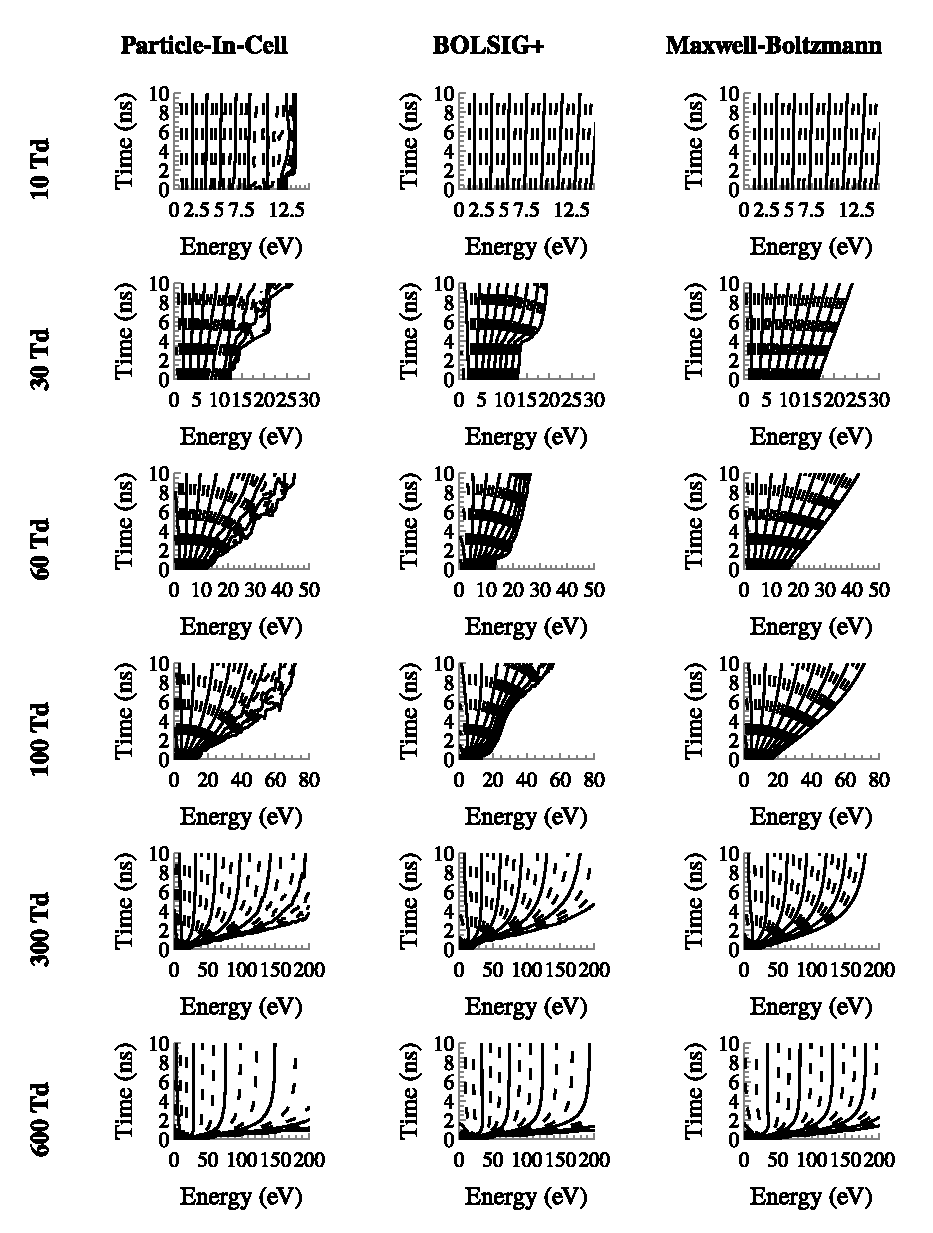
\includegraphics{./chapters/modeling/figures/picmb.eps}
  \caption{Contour plots of the \acs{eedf}s determined from \acs{pic}
    simulations, and the corresponding Maxwell-Boltmzann distributions for a range
    of electric fields.}
  \label{fig:picmb}
\end{figure}
as a series of contour plots. The jaggedness of the \acs{pic} simulations
results from the finite number of particles in the system and the low
probability of high energy electrons. This problem is ameliorated at higher
electric fields where the probability of high-energy electrons increases. It is
also helped by the ionization processes which begin to occur after the first few
nanoseconds.

At 10 Td, the \acs{eedf}s are relatively unchanged over the duration of the
simulation. The subtle slopes of the contours suggest a small increase in the
overall temperature and energy of the system as a function of time. This is more
noticeable at 30 Td, where the contours have a more distinct slope. The spacing
between the slopes is relatively constant for each case--equivalent to a
Maxwell-Boltzmann distribution. However, there is some deviation at low energies
in the case of the BOLSIG+ solutions.

At 60 and 100 Td, the \acs{pic} results begin to exhibit contour spacings which
are consistent at low energies, but begin to grow at higher energies. This is
evidence of a growing population of high-energy electrons, in excess of what
exists in a Maxwell-Boltzmann distribution. Interestingly, the BOLSIG+ solutions
exhibit unique contour shapes which are inconsistent with the other two cases.
Additionally, the spacing of the contours is less consistent, and there is a
dearth of high energy electrons compared to the other cases.

By 300 and 600 Td the situation is reversed, as the Maxwell-Boltzmann
distributions begin to underestimate the population of high energy electrons.
Examination of the individual distributions shows that the \acs{pic} \acs{eedf}s
have a larger population of low energy (less than 20 eV) and high energy
(greater than 100 eV) electrons. This can be explained by the general shape of
the cross sections. The only reactions available to electrons in the \acs{pic}
simulations are elastic scattering, excitation (19.6 eV threshold), and
ionization (24.6 eV threshold). As the inelastic processes turn on at energies
in excess of the 20 eV, the electron population begins to be depleted. Likewise,
the electron population begins to rebound at higher energies as the cross
sections fall off.

Unlike Starikovskaia and Starikovskii's results \cite{Starikovskaia2001} the
various approaches produce comparable \acs{eedf}s. Generally, the
Maxwell-Boltzmann results provide the best match to the \acs{pic} simulations at
electric fields of 100 Td and below. Conversely, the BOLSIG+ results better
represent the \acs{eedf} past 100 eV at the higher field values. That said,
these electrons do not provide a large contribution to the excited states of the
plasma. They are well past the excitation and ionization cross section peaks and
are relatively few in number. Given the larger computational burden of the
Boltzmann solver and the small perceived benefit, it was concluded that the that
the Maxwell-Boltzmann distributions provided an adequate representation of
the \acs{eedf} for the global model.

\subsection{Energy Equation}

The \acs{eedf} provides a means by which to calculate the rate coefficients in
equation~\ref{eq:gcont}. However, as was seen in figure~\ref{fig:picmb}, the
distribution function changes over time. Previously, the \acs{pic} simulations
were used to calculate the time evolution of the mean electron energy, but an
alternate approach was required for the global model.

With suitable assumptions, equation~\ref{eq:energy} (the second moment of the
Boltzmann equation) can provide the means to evolve the mean energy with each
time step. Given the assumptions underlying the global model, the spatial
derivatives can be neglected such that
\begin{equation}
  \frac{d}{dt}\left(\frac{3}{2}p_e\right) =
  \frac{d}{dt}\left(\frac{3}{2}p_e\right)\bigg|_\mathrm{coll}.
\end{equation}
Using the isothermal equation of state \cite{Lieberman2005}, $p=n\kB T$, this
can be rewritten as,
\begin{equation}
  \frac{d}{dt}\left(\frac{3}{2}n_e\kB T_e \right) =
  \frac{d}{dt}\left(\frac{3}{2}n_e\kB T_e \right)\bigg|_\mathrm{coll}.
  \label{eq:energy2}
\end{equation}
The term on the RHS is the collision operator which expresses energy gained or
lost by electrons\footnote{In some plasmas, it is desirable to also treat gas
heating with a similar equation as it can have an appreciable impact on certain
rate constants. However, as noted in Chapter~\ref{chp:metastables}, the gas
temperature of the \acs{rpdn} in question remains at room temperature.} in
particle collisions.

Several different types of energy transfer were considered by the global model.
The first was the heating caused by the electric field. This was followed by
electron energy losses as a result of elastic scattering by the atoms. Finally,
inelastic collisions with all helium states through $n=4$ were considered.
Together, these phenomena replace the term on the RHS of
equation~\ref{eq:energy2} with,
\begin{equation}
  \frac{e^2n_eE(t)^2}{m_ek_m(T_e)N_g}
  - n_ek_m(T_e)N_g\left(\frac{3m_e}{M}\right)\frac{3}{2}\kB(T_e-T_g)
  - n_e \sum_i \sum_{j\neq i} K^e_{ij}N_i\Delta\epsilon_{ij},
  \label{eq:energyparts}
\end{equation}
where $E(t)$ is the time-varying electric field, $k_m$ is the electron momentum
transfer frequency from Pack et al. \cite{Pack1992}, and $\Delta\epsilon_{ij}$
is the energy lost or gained by the electron in atomic (de)excitation reactions.
The first term includes the DC conductivity \cite{Lieberman2005} of the plasma,
and accounts for the heating of the electrons by the electric field. The second
term is the elastic cooling of the electrons by the neutral atoms, where the gas
temperature. The third term is the energy gained or lost by the electrons in
atomic (de)excitation reactions. The
equations~\ref{eq:energyparts},~\ref{eq:energy2} and~\ref{eq:gcont} form the
main components of the global model. Together they provide the means to solve
for the evolution of the electron temperatures, electron densities, excited
state densities, and plasma emissions as functions of time.

\subsection{Model Solutions}

For the purposes of computation, equation~\ref{eq:gcont} can be rewritten for
each atomic state, $i$, resulting in a set of linear, first order differential
equations,
\begin{multline}
  \frac{d}{dt}
  \begin{pmatrix}
    N_1 \\
    N_2 \\
    \vdots \\
    N_M
  \end{pmatrix}
  = n_e
  \begin{pmatrix}
    -\sum_{j\neq 1}K^e_{1,j} & K^e_{2,1}      & \hdots & K^e_{M,1} \\
    K^e_{1,2}      & -\sum_{j\neq 2}K^e_{2,j} & \hdots & K^e_{M,2} \\
    \vdots         & \vdots         & \ddots & \vdots    \\
    K^e_{1,M}      & K^e_{2,M}      & \hdots & -\sum_{j\neq M}K^e_{M,j}
  \end{pmatrix}
  \cdot
  \begin{pmatrix}
    N_1 \\
    N_2 \\
    \vdots \\
    N_M
  \end{pmatrix} \\
  +
  \begin{pmatrix}
    0      & K^o_{2,1}              & \hdots & K^o_{M,1} \\
    0      & -\sum_{j < 2}K^e_{2,j} & \hdots & K^o_{M,2} \\
    \vdots & \vdots                 & \ddots & \vdots    \\
    0      & 0                      & \hdots & -\sum_{j < M}K^e_{M,j}
  \end{pmatrix}
  \cdot
  \begin{pmatrix}
    N_1 \\
    N_2 \\
    \vdots \\
    N_M
  \end{pmatrix} \\
  + N_g
  \begin{pmatrix}
    -\sum_{j\neq 1}K^a_{1,j} & K^a_{2,1}      & \hdots & K^a_{M,1} \\
    K^a_{1,2}      & -\sum_{j\neq 2}K^a_{2,j} & \hdots & K^a_{M,2} \\
    \vdots         & \vdots         & \ddots & \vdots    \\
    K^a_{1,M}      & K^a_{2,M}      & \hdots & -\sum_{j\neq M}K^a_{M,j}
  \end{pmatrix}
  \cdot
  \begin{pmatrix}
    N_1 \\
    N_2 \\
    \vdots \\
    N_M
  \end{pmatrix}, \\
\end{multline}
where $M$ is the total number of atomic states and $\epsilon_i <
\epsilon_{i+1}$. An additional equation can be added to separately account for
electrons as well as electron-specific processes, however the global model used
here assumed quasineutrality by enforcing the relation $N_\mathrm{ion}=n_e$.
Changes in the density of each atomic state were calculated by numerical
integration of these equations. The range of time scales exhibited by the
\acs{rpnd} made it desirable to implement adaptive control of the time step
size. For this reason, the Runge-Kutta-Fehlberg method, adapted from Bradie
\cite{Bradie2006}, was used as the integration scheme.

Initial metastable densities were determined from the \acs{las} measurements and
initial electron densities were determined from \acs{lcif} measurements made by
Weatherford \cite{Weatherford2012a}. However, the \acs{lcif} electron density
measurements were only available for 1.0, 4.0, and 8.0 Torr. Therefore,
subsequent analyses only consider these conditions. Sensitivity to changes in
the initial electron density will be addressed in the following section.

No measurements of the electron temperature in the pre-pulse period were
available. Therefore, it was necessary to assume an electron temperature. Given
the relatively long period of time between pulses, an in initial temperature of
0.2 eV was used. Exploratory simulations found that changes in the initial
electron temperature had a negligible impact on the final distribution of
excited states. Initial excited state densities (not including ions and
metastables) were determined by their values in equilibrium with the 0.2 eV
electrons. Per the results from Chapter~\ref{chp:metastables}, the neutral gas
temperature was fixed at 300 K for the duration of the simulation.

Despite access to the waveform of the applied potential, the actual
time-evolution of the electric field at the metastable measurement points is not
well known. This is a result of the distinctly nonlinear impedance of the
\acs{rpnd} plasma. Takashima et al.\ performed measurements of the electric
field in a \acs{fiw} using a capacitive probe and found it to be significantly
different from the vacuum field. Separately, Ito et al. \cite{Ito2010} and
M\"{u}ller et al. \cite{Muller2011a}, measured the electric fields in a
\acs{rpnd} with a 1.2 mm gap between parallel electrodes using a wave-mixing
approach. They too found a large difference between the vacuum field and the
actual field.

In all three cases, the evolution of the electric field could be best described
by a Gaussian-like pulse, followed by a small, persistent electric field. This
persistent field was on the order of 20-25\% of the peak field value, and would
remain for at least several tens of nanoseconds. The total duration and
magnitude of the persistent field varied between studies and some, such as the
work of Anikin et al. \cite{Anikin1998}, did not appear to record it. Given the
uncertainty associated with the nature of this persistent field, the global
model simulations only considered a single Gaussian pulse. The time domain of
the simulations covered 190 ns with the peak of the pulse centered at 40 ns.

\section{Perturbation Study}

The input values for the global model were relatively fixed, with the exception
of the peak electric field and the width of the pulse. It was initially expected
that the pulse-width would be approximately equal to the width of the applied
pulse, 25 ns. The global models were matched to the metastable measurements by
iterative adjustment of the peak electric field and the pulse-width. However,
there was no clear means by which to estimate the error in the global model
calculations.

In order to provide a partial quantization of this error, a preliminary fit of
the 4.0 Torr data was made and used as a benchmark. Subsequent simulations were
run with small perturbations to the peak electric field, pressure, pulse-width,
and initial electron density. In each case, the benchmark value was perturbed by
$\pm10\%$.

The nominal conditions of the simulation are recorded in table~\ref{tbl:nominal}
\begin{table}
  \centering
  \caption{Nominal simulation parameters for the 4.0 Torr operating condition.}
  \begin{tabular}{llll}
    \toprule
    Pressure & Initial Electron    & Pulse      & Peak Electric \\
    (Torr)   & Density (m$^{-3}$)  & width (ns) & Field (Td)\\ 
    \midrule
    4.0      & 5.36$\times10^{13}$ & 40         & 207 \\
    \bottomrule
  \end{tabular}
  \label{tbl:nominal}
\end{table}
and results of these simulations are shown in figure~\ref{fig:perturbed}.
\begin{figure}
  \centering
  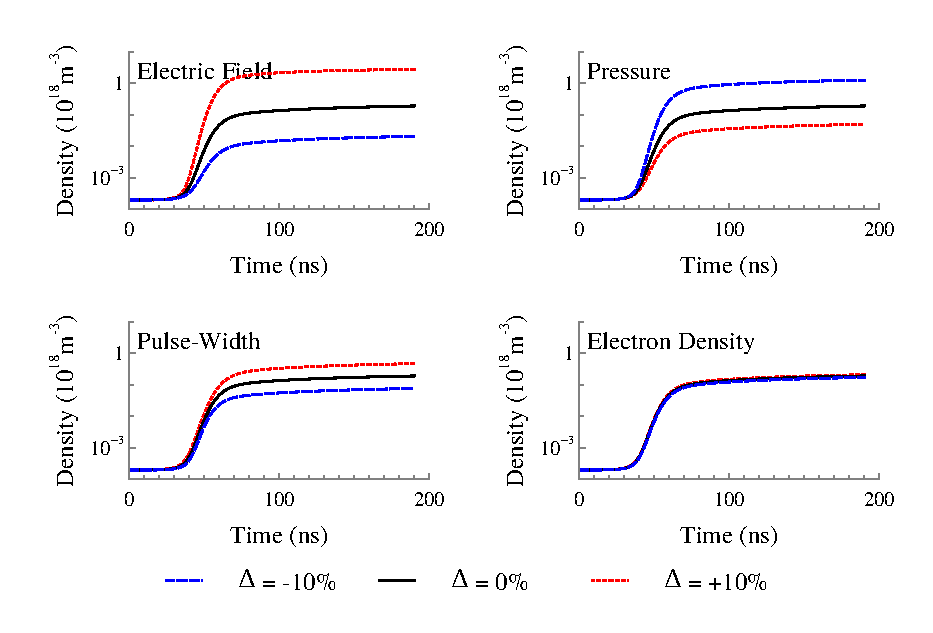
\includegraphics{./chapters/modeling/figures/perturbed.eps}
  \caption{Simulations showing the effects of perturbations to the initial
  conditions on the metastable dynamics.}
  \label{fig:perturbed}
\end{figure}
The metastable trends suggest that the initial electron density has a relatively
small impact on the metastable dynamics. Closer examination reveals that the
final metastable densities change by approximately $\pm10\%$, almost one-to-one
with the initial electron density. In contrast, changes to the pulse-width
produce much more significant changes in the metastable densities. As the
pulse-width is increased, the metastable densities increase. Knowing that the
electric field is fixed, this change can be attributed to the increase in energy
deposited in the electron population.

The two largest factors in the determination of the metastable densities were
the neutral gas pressure and the electric field. The perturbations to these
quantities resulted in largest changes in the final metastable densities. As can
be seen in figure~\ref{fig:perturbed}, increases in pressure corresponded to a
decrease in metastable densities. Changes to the neutral gas pressure tend to
affect the system via several different mechanisms. As seen in
equation~\ref{eq:energyparts}, increases to the gas pressure tend to decrease
the energy deposited in the electrons, and increases losses due to elastic
scattering, thus reducing the energy that can be deposited in excited states.
This competes with the increased number of ground state atoms available for
excitation. That the increase in gas pressure results in a reduced metastable
density indicates that the reduced energy deposition in the electrons is more
important than the increased availability of neutral atoms.

The large impact of the electric field can be traced back to changes in the
ionization rate for each condition. As seen in figure~\ref{fig:ionrates},
\begin{figure}
  \centering
  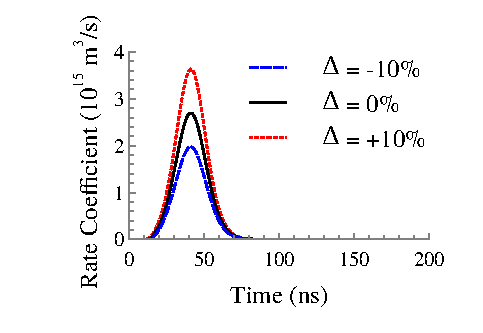
\includegraphics{./chapters/modeling/figures/ionrates.eps}
  \caption{Ionization rates coefficients corresponding to the perturbed electric
  field simulations.}
  \label{fig:ionrates}
\end{figure}
the magnitude of the ionization rate coefficient corresponds to the magnitude of
the electric field. While the changes are somewhat modest, as seen in
Chapter~\ref{chp:theory}, ionization processes exponentially with time. This
means that small changes to the rate coefficient manifest as large differences
in the final electron density. Since the rate of metastable generation is
proportional to the electron density, these changes to the electron density
equate to changes in the metastable density.

\section{Plasma Dynamics}

The plasma dynamics for the 1.0, 4.0, and 8.0 Torr conditions were obtained by
iteratively matching the pulse-width and peak electric field to the metastable
density immediately before the arrival of the reflected pulse. The process was
somewhat complicated by the fact that multiple combinations of the peak field
and pulse-width could produce the same metastable density. Therefore, it was
necessary to fix or otherwise predict one of the values.

Of the two, the pulse-width was the most promising to eliminate as a variable.
The characteristics of the applied pulse already provide reasonable bounds on
the possible widths. Therefore, the 4.0 Torr condition was simulated with a
range of pulse-widths from 5-50 ns with the peak field selected to produce the
same final metastable density in each case. 

The metastable density trend for each pulse-width is compiled in
figure~\ref{fig:widths}.
\begin{figure}
  \centering
  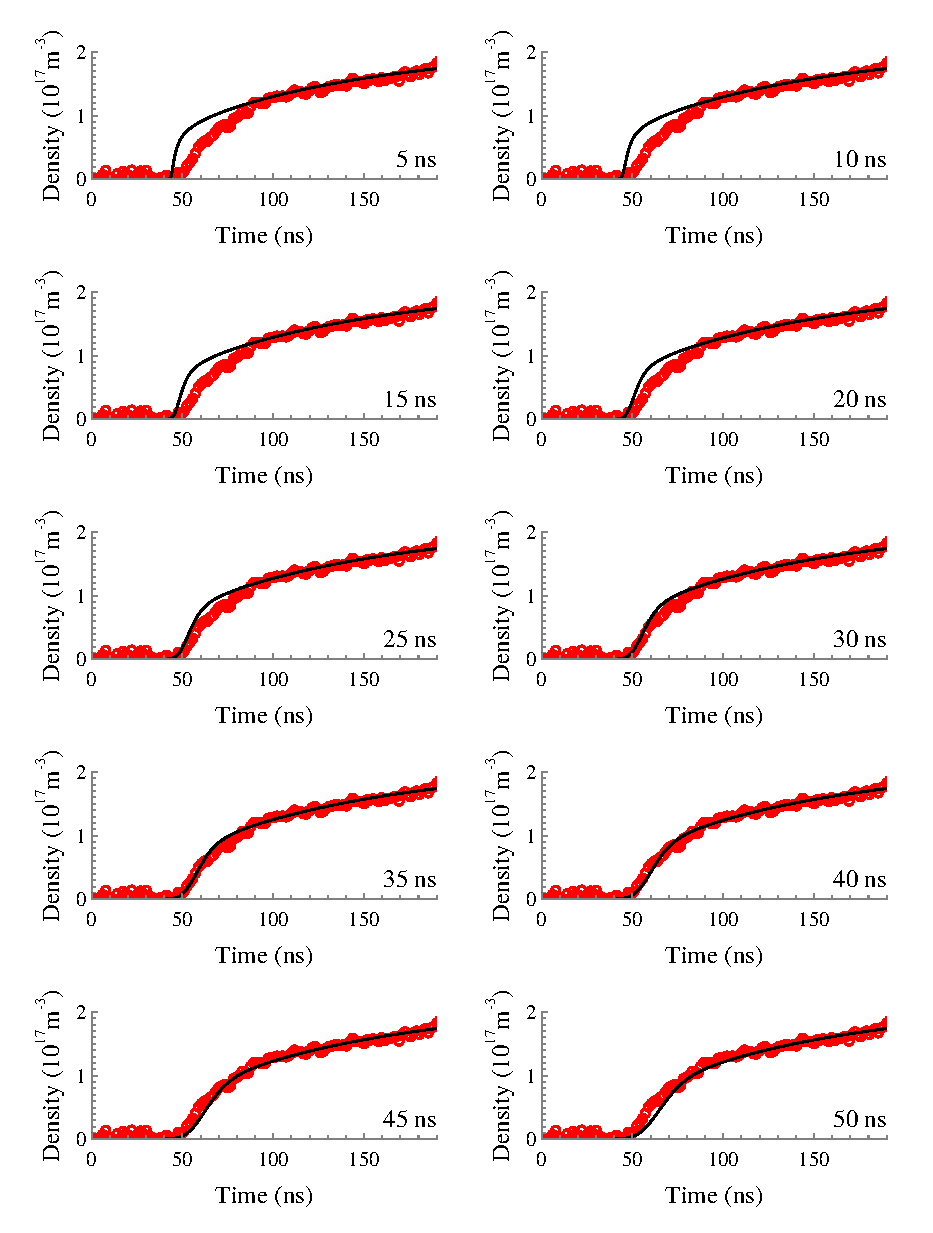
\includegraphics{./chapters/modeling/figures/widths.eps}
  \caption{Comparison of measured metastable values (represented by open
    circles) to simulations with a range of pulse-widths.}
  \label{fig:widths}
\end{figure}
It is immediately apparent that the short pulse-widths do not provide an optimal
description of the data. Even the metastable densities for the 25 ns simulation
grow significantly faster than those of the experiment. The experimental limit
on the time resolution was the photodiode, with a response time of 5 ns,
therefore the slow rise of the metastable states appears to be a real phenomena.
This suggested that the effective pulse-width in the \acs{rpnd} extended longer
than the duration of the applied voltage. Indeed, the best match of the data for
the illustrated simulations occurs for a pulse-width of 40 ns.

The results of the pulse-width comparison suggest that additional excitation is
taking place in addition to the applied pulse. In order to determine the origin
of this excitation, a survey was made of the neutral emissions spectra. The
details of these measurements will be discussed in more detail in
Chapter~\ref{chp:emissions}. The strongest signal was observed at 396 nm,
corresponding to the 4$^1$P$^\mathrm{o}$-2$^1$S transition. Measuring these
emissions as a function of time produced figure~\ref{fig:double}
\begin{figure}
  \centering
  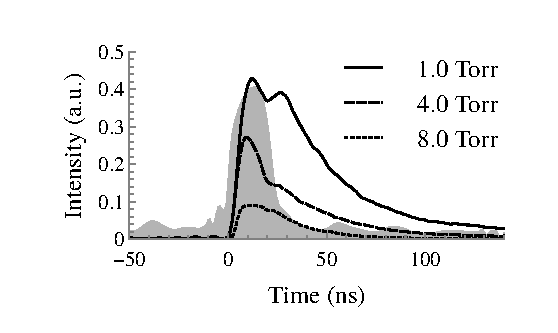
\includegraphics{./chapters/modeling/figures/double.eps}
  \caption{Evidence of return stroke in the double-peaking of plasma emissions.}
  \label{fig:double}
\end{figure}
where the emissions for each operating condition have been overlaid on the
applied voltage pulse. The voltage pulse clearly coincides with an initial
increase in the number of helium atoms in the 4$^1$P$^\mathrm{o}$ state. 15 ns
later, another increase is visible, particularly at 1.0 and 4.0 Torr. This
second transient is similar to the return strokes observed in early streamer
research \cite{Snoddy1936, Loeb1940, Mitchell1947}. The observation of return
strokes in similar, contemporary studies \cite{Vasilyak1994, Pai2009,
Starikovskiy2013} suggests that this is a reasonable explanation for the
double-peaked emissions. If the forward and return stroke possess durations
equal to the applied voltage (25 ns), separated by 15 ns, then the excitation
period would be approximately 40 ns. This is consistent with the pulse-width
required to match the observed data. For this reason, a pulse-width of 40 ns was
used for all subsequent simulations.

Figure~\ref{fig:fieldtau}
\begin{figure}
  \centering
  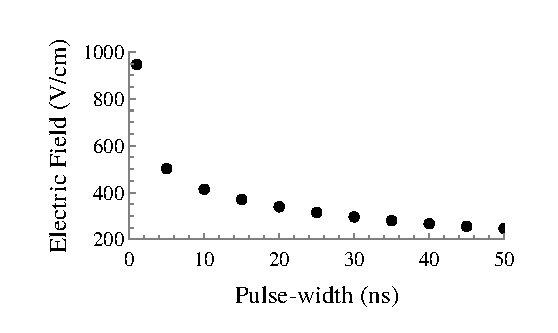
\includegraphics{./chapters/modeling/figures/fieldtau.eps}
  \caption{The required peak field strengths as a function of the pulse-width.}
  \label{fig:fieldtau}
\end{figure}
is a scatter plot of the peak electric fields necessary to obtain the same final
metastable density as a function of the pulse-width. Initially, as the
pulse-width is decreased from 50 ns, only small increases of the electric field
are required to obtain the same number of metastable atoms by the end of the
simulation period. However, as the pulse-width is decreased further, the rate at
which the electric field must increased grows substantially.

Eventually, it is no longer possible to maintain the same metastable density,
despite further increases in the electric field. This occurs for the same reason
that the \acs{eedf} from the \acs{pic} simulations was depressed between 20 and
100 eV--eventually, the cross sections fall off with increasing electron energy.
This places an upper limit on the rate coefficient as a function of electron
temperature. Figure~\ref{fig:longrates}
\begin{figure}
  \centering
  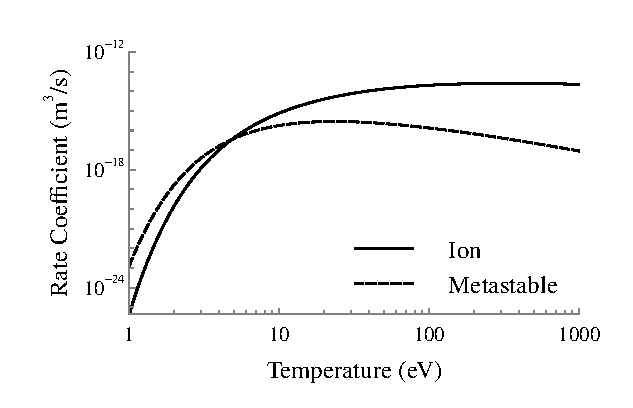
\includegraphics{./chapters/modeling/figures/longrates.eps}
  \caption{Ionization and metastable rate coefficients as functions of
    electron temperature.}
  \label{fig:longrates}
\end{figure}
shows the ionization and metastable rate coefficients as functions of the
electron temperatures in the system. The ionization rate coefficient peaks at
approximately 320 eV, while the metastable rate coefficient peaks much lower at
around 23 eV. These rate coefficients, along with the general form of the cross
sections for the reactions, show that there is an optimal field strength for
ionization and excited state generation. Further increases in the electric field
would only serve to reduce to reduce the final density of these particles.
However, there may still be additional benefits in a higher electric field. The
runaway electrons which can be generated at these field strengths, described by
Vasilyak \cite{Vasilyak1994} among others, could help increase the discharge
volume and homogeneity via nonlocal energy deposition.

Figure~\ref{fig:nmcomp}
\begin{figure}
  \centering
  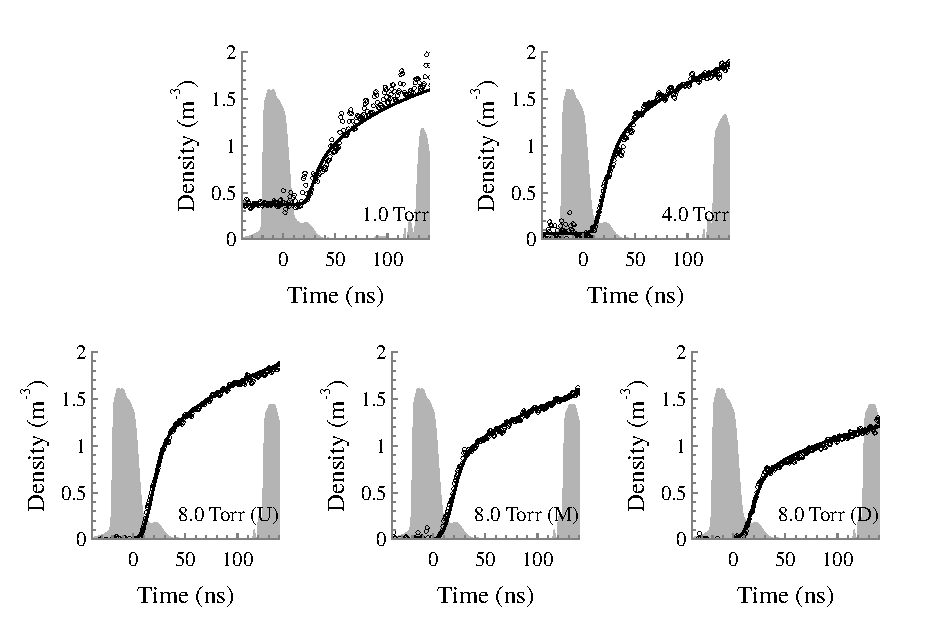
\includegraphics{./chapters/modeling/figures/nmcomp.eps}
  \caption{Comparison of the measured metastable densities (open circles) to
    the global model simulations. The shaded region illustrates the applied
    voltage pulse. The parentheses following the 8.0 Torr labels indicate the
    axial location of the measurement.}
  \label{fig:nmcomp}
\end{figure}
shows the comparison of the measured metastable densities for 1.0, 4.0, and 8.0
Torr. As seen in chapter~\ref{chp:metastables}, there was little axial variation
in the metastable measurements at 1.0 and 4.0 Torr. For this reason, simulations
were conducted only for the measurements at the midstream positions. In
contrast, the axial distribution of metastables showed noticeable variation at
8.0 Torr. Therefore, each location was considered independently in the
simulations.

Despite the assumptions involved in the development of the global model, the
simulation results show impressive agreement with the measurements. This
includes the period of 0-40 ns when the metastable growth rate is the largest.
The plasma behavior in during this time is dominated by energetic electrons that
have been accelerated by the large electric fields. Given the relatively short
time period, inter-atomic and radiative processes play a relatively unimportant
role. The most significant discrepancies appear in the 1.0 Torr simulations
where the global appears to overestimate the metastable density during the
pulse.

The global model also performs well in the afterglow period, from 40 ns to the
end of the measurements. After the pulse, the electrons begin to undergo rapid
cooling, as seen in figure~\ref{fig:etemps}.
\begin{figure}
  \centering
  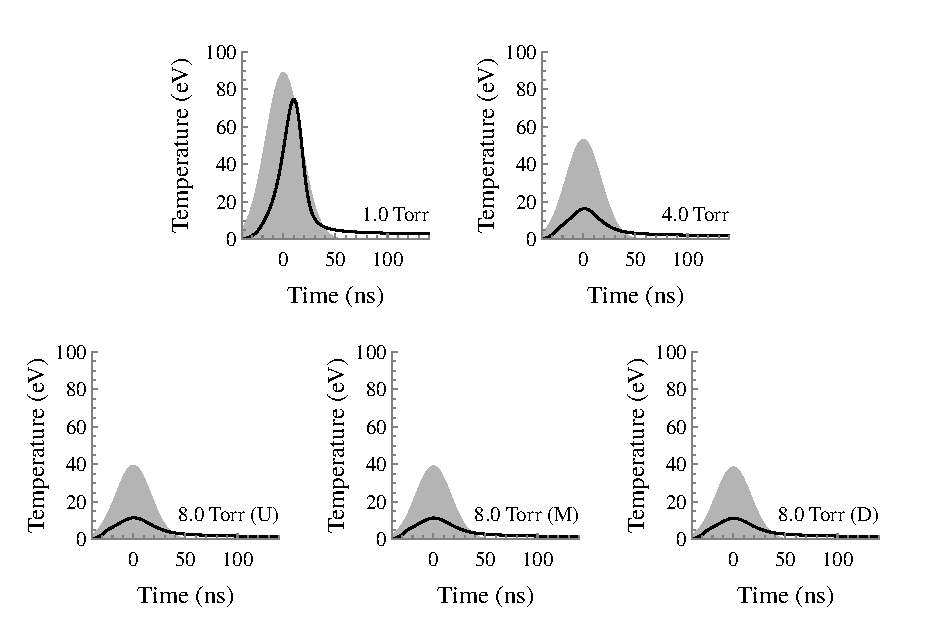
\includegraphics{./chapters/modeling/figures/etemps.eps}
  \caption{Global model predictions of the electron temperatures at the
  simulated conditions, overlaid on the corresponding electric field.}
  \label{fig:etemps}
\end{figure}
By 50 ns, the electron temperatures have fallen below 10 eV in all cases, and by
the end of the simulation they are all below 3 eV. As a result of this rapid
cooling, the rate of electron-induced reactions falls significantly. As was seen
in figure~\ref{fig:longrates}, the rate for metastable and ion generation begin
to undergo a fast decline at temperatures below 10 eV. This indicates that much
of the metastable growth after 50 ns can be attributed to radiative transitions
from upper excited states. Again, the most significant discrepancies appear for
the measurements at 1.0 Torr. In this case, the simulations appear to
underestimate the total metastable population.

The issues in accurately simulating the 1.0 Torr case may be a result of the
large electric field present in the system. As can be observe in
table~\ref{tbl:simsum}
\begin{table}
  \centering
  \caption{Summary of the peak values for several plasma parameters from the
  global model simulations.}
  \label{tbl:simsum}
  \begin{tabular}{lllll}
    \toprule \\
    Pressure         & E/N  & T$_\mathrm{e}$ & N$_\mathrm{m}$ & n$_\mathrm{e}$ \\
    (Torr)           & (Td) & (eV)           &  (m$^{-3}$)    & (m$^{-3}$) \\
    \midrule \\
    1.0              & 346  & 74.6           & 1.62$\times10^{17}$ & 
      5.06$\times10^{17}$ \\
    4.0              & 207  & 16.3           & 1.87$\times10^{17}$ &
      3.36$\times10^{17}$ \\
    8.0 (Upstream)   & 154  & 11.5           & 1.88$\times10^{17}$ &
      2.57$\times10^{17}$ \\
    8.0 (Midstream)  & 152  & 11.4           & 1.57$\times10^{17}$ & 
      2.14$\times10^{17}$ \\
    8.0 (Downstream) & 150  & 11.3           & 1.21$\times10^{17}$ &
      1.65$\times10^{17}$ \\
    \bottomrule
  \end{tabular}
\end{table}
the electric field approaches 350 Td for the 1.0 Torr discharge. This
corresponds to the regime in which the Maxwell-Boltzmann distribution (as well
as the BOLSIG+ results) begin to deviate from the \acs{pic} predictions.
Specifically, the Maxwell-Boltzmann distribution tended to overestimate the
number of electron in the range of 20-100 eV at high electric fields. These are
precisely the electrons which are responsible for the generation of the
metastable states. This suggests that the assumption of a Maxwell-Boltzmann
distribution would tend to overestimate the metastable generation at large
electric fields, consistent with what is observed in figure~\ref{fig:nmcomp}.

As the pressure is increased, the electric field required to match the measured
metastable densities begins to decrease, though the final metastable densities
remain approximately the same.

\begin{figure}
  \centering
  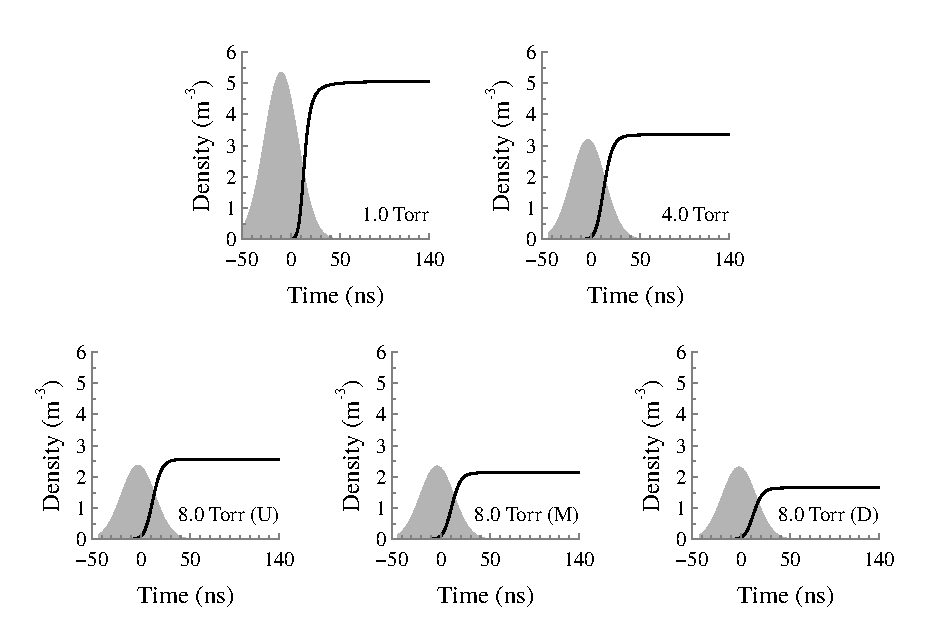
\includegraphics{./chapters/modeling/figures/necomp.eps}
  \caption{Global model predictions of the electrons densities at the simulated
  conditions.}
  \label{fig:necomp}
\end{figure}







\section{Summary}




  \chapter{Population Kinetics}\label{chp:emissions}
    The global model was used to infer the electric field, electron densities, and
electron temperatures in the \acs{rpnd} from the metastable measurements.
However, as was described in the development of the model, it is also capable of
predicting the densities of other excited states and the optical emissions of
the \acs{rpnd}. This chapter will describe the measurement of the optical
emissions of the \acs{rpnd} and then the use of these measurements to determine
the \acs{rpnd} wave velocity and electrons temperatures. Finally, the electron
temperatures and the spectral trends will be compared to those obtained from the
global model.

\section{Emission Measurements}

Emissions spectroscopy was conducted at the same operating conditions as the
metastable measurements. Light collection was accomplished with a 1 cm diameter
bundle of optical fibers, butted against the outside of the glass envelope. The
other end was placed at the entrance slit of a ISA Jobin-Yvon SPEX HR460
monochromator. A grating with 1200 grooves/mm was installed in the
monochromator. The entrance slit width was set to 250 $\mu$m and the exit slit
was set at 500 $\mu$m. This was done so as to collect the integrated intensity
of each spectral line.

A photomultiplier tube (\acs{pmt}) of model C31034 was used to record the
changes in intensity over time. The tube voltage was set to 1900 V and was
terminated into a 50 $\Omega$ resistor. Specifications could not be found for
the tube, however measurements demonstrated a rise time of, at most, 3.5 ns.
Unlike the laser-absorption spectroscopy measurements, each emission curve was
averaged over 1000 acquisitions and 5 $\mu$s. Otherwise, the acquisition
settings remained the same.

The range of spectral sensitivity for the photocathode of the \acs{pmt} limited
measurements to transitions occurring between 350-750 nm. The list of observable
transitions is recorded in table~\ref{tbl:transitions}.
\begin{table}
  \centering
  \caption{Table of the observed optical transitions and their transition
    rates.}
  \begin{tabular}{lllll}
    \toprule                                                                    \\
    Initial      & Final        & Wavelength &              &                   \\
    State        & State        & (nm)       & A (s$^{-1}$) & $\sum$A (s$^{-1}$)\\
    \midrule                                                                    \\
    3$^3$P$\odd$ & 2$^3$S       & 388.97     & $9.46\EE6$   & $1.06\EE7$        \\
    4$^1$P$\odd$ & 2$^1$S       & 396.59     & $6.95\EE6$   & $2.52\EE8$        \\
   %5$^3$D       & 2$^3$P$\odd$ & 402.73     & $1.16\EE7$   & $1.64\EE7$        \\
    4$^3$D       & 2$^3$P$\odd$ & 447.28     & $2.46\EE7$   & $3.12\EE7$        \\
   %4$^3$S       & 2$^3$P$\odd$ & 471.45     & $9.52\EE6$   & $1.60\EE7$        \\
    4$^1$D       & 2$^1$P$\odd$ & 492.33     & $1.99\EE7$   & $2.70\EE7$        \\
    3$^1$P$\odd$ & 2$^1$S       & 501.71     & $1.34\EE7$   & $5.80\EE8$        \\
    3$^3$D       & 2$^3$P$\odd$ & 587.73     & $7.07\EE7$   & $7.07\EE7$        \\
    3$^1$D       & 2$^1$P$\odd$ & 668.00     & $6.37\EE7$   & $6.37\EE7$        \\
    3$^3$S       & 2$^3$P$\odd$ & 706.72     & $2.79\EE7$   & $2.79\EE7$        \\
    3$^1$S       & 2$^1$P$\odd$ & 728.34     & $1.83\EE7$   & $1.83\EE7$        \\
  \end{tabular}
  \label{tbl:transitions}
\end{table}
Several factors, including the fiber, monochromator grating, and the
photocathode coating resulted in a nonuniform response with wavelength. This was
compensated for with spectral measurements of an Optronic Laboratories M-1179
spectral irradiance standard, powered by an Optronic Laboratories OL 65 power
supply. 

\section{Wave Velocities}

In the analysis of \acs{fiw} discharges, one of the most common means of
comparison is the use of wave velocities. In the studies reported by Vasilyak
\cite{Vasilyak1994}, the velocities were measured using several approaches. In
one, capacitive probes were placed in contact with the dielectric of the
discharge tube, and the time delay between the voltage signals was used as the
wave velocity. In some cases an intensified \acs{ccd} was used to track the
propagation of the wave. Alternately, a photomultiplier tube was positioned
against the dielectric at varying axial locations. This is the approach used
here.

The maximum detectable velocity was limited by several factors. Data were only
available at intervals of 1 ns. As the maximum separation of measurement
locations was 15.24 cm, this set an upper limit of about 1.5$\times10^8$ m/s.
Additional limitations were imposed by the jitter of the pulser output. Overall,
the maximum detectable wave velocity was $5.0\times10^7$ m/s.

The velocities were determined as an average of the all the emission curves
recorded. In each case, the curve at each axial location was interpolated with a
smoothing spline. The time of the maximum derivate of the emission curves was
used as the reference point in each case. The distance between the measurement
locations was then divided by the time delay between the maximum derivatives.
The results of these calculations are recorded in table~\ref{tbl:velocities}.
\begin{table}
  \centering
  \caption{Wave velocities in the \acs{rpnd}.}
  \label{tbl:velocities}
  \begin{tabular}{lll}
    \toprule                                                      \\
    Pressure  & Upstream                & Downstream              \\
    (Torr)    & Velocity (m/s)          & Velocity (m/s)          \\
    \midrule                                                      \\
    8.0       & $3.01\pm1.21\times10^7$ & $1.73\pm0.26\times10^7$ \\
    16.0      & $1.46\pm0.19\times10^7$ & $6.80\pm1.75\times10^6$ \\
  \end{tabular}
\end{table}

Delays in the emissions at the different axial locations only appeared for the
8.0 and 16.0 Torr conditions. The propagation of the discharge across the
chamber was essentially instantaneous for all other conditions. Vasilyak et al.\
note that it is difficult to compare the velocities of \acs{fiw} discharges as a
result of numerous dependencies and poorly understood physics. In the \acs{fiw},
the velocity varies with pressure, gas, outer dielectric, pulse voltage, and
preionization. There is no reason to suspect that the situation is any different
for the \acs{rpnd}. That said, the measured values fall within the wide range
that has previously been associated with streamers, \acs{fiw}s, and \acs{rpnd}s.

The early work of Schonland and Collens \cite{Schonland1933} determined that the
luminous front of lightning propagated with a velocity of $0.72-5.3\times10^7$
m/s for the forward and return stroke. The studies reported by Vasilyak et al.
\cite{Vasilyak1994} give a range of approximately $2-5\times10^7$ m/s for a 200
kV \acs{fiw} in helium at pressures from 0.1-760 Torr. Propagation velocities
for atmospheric plasma jets of helium have been measure at about $10^5$ m/s
\cite{Lu2006} with simulations providing confirmation \cite{Naidis2010} of these
values. Fast imaging by Ito et al. \cite{Ito2010} determined a velocity of
$10^6$ m/s for a hydrogen \acs{rpnd}.


\section{Electron Temperatures}

Measurement of the electron temperature in \acs{rpnd}s poses a large difficulty
for several reasons. The most significant of which is the concept of temperature
itself. As was noted in Chapter~\ref{chp:modeling}, the \acs{rpnd} is a highly
dynamic system which does not necessarily result in a population of electrons
with a Maxwell-Boltzmann distribution. In the absence of this property, the
``temperature'' quantity can have an ambiguous meaning. Often, the reported
temperature describes the Maxwell-Boltzmann distribution which best matches
measured some choice of plasma properties (such as plasma emissions). In other
cases, the temperature may describe the mean electron energy of the \acs{eedf},
such as in Chapter~\ref{chp:modeling} or in the work of Starikovskaia and
Starikovskii \cite{Starikovskaia2001}.

The temperatures generated in these two cases will coincide only for a limited
number of situations and the choice of diagnostics. Thus, it is of interest to
search for useful electron temperature diagnostics which apply to the
\acs{rpnd}. The electron temperature of a system is most often determined by the
use of electrostatic probes, such as those discussed by Lieberman
\cite{Lieberman2005}. However, as was discussed at the beginning of
Chapter~\ref{chp:metastables}, physical probes are not a reasonable option of
the \acs{rpnd}. An active optical technique, such as Thomson scattering
\cite{VanGessel2012}, would be an ideal solution if the electron densities in
the \acs{rpnd} were not below its sensitivity threshold.

Therefore, several attempts were made to translate the plasma emission
measurements to electron temperatures. Such techniques have been successful in
the analysis of steady-state systems with relatively low electron densities,
however the applicability to very dynamic discharges is not a given and must be
qualified \cite{Kunze2009}. 

\subsection{Boltzmann Plots}

When the population of two excited states are in equilibrium with the electrons,
the ratio of their densities can be written as \cite{Griem2005}
\begin{equation}
  R = \frac{\lambda_{i,j}A_{i,j}g_j}{\lambda_{i',j'}A_{i',j'}g_{j'}}
      \exp\left( -\frac{\Delta\epsilon_{i,j} - \Delta\epsilon_{i',j'}}
                       {\kB T_e} \right),
\end{equation}
where the subscripts represent different electronic states, $\lambda$ is the
transition wavelength, $A$ is the spontaneous transition rate, $g$ is
statistical degeneracy, and $\Delta\epsilon$ is the energy separation between
the identified states. In this case, the line ratios only depend on the electron
temperature and physical quantities that are well-tabulated for helium.

This approach can be applied to several successive transitions by plotting the
quantity
\begin{equation}
  \log\left(\frac{I_{i,j}\lambda_{i,j}}{g_jA_{ij}}\right)
\end{equation}
with respect to $\Delta\epsilon_{i,j}$, where $I$ is the measured intensity of
the optical transition. Ideally, the plotted points would form a line where the
negative reciprocal is equal to the electron temperature. This is most
frequently referred to as a Boltzmann plot. 

The emissions data for the wavelengths recorded in table~\ref{tbl:transitions}
was compiled into a series of intensities for each time step. A Boltzmann plot
was then generated for each time step and a line was fit to the data using a
least-squares algorithm. This produced the temperature estimates seen in
figure~\ref{fig:boltcomp}.
\begin{figure}
  \centering
  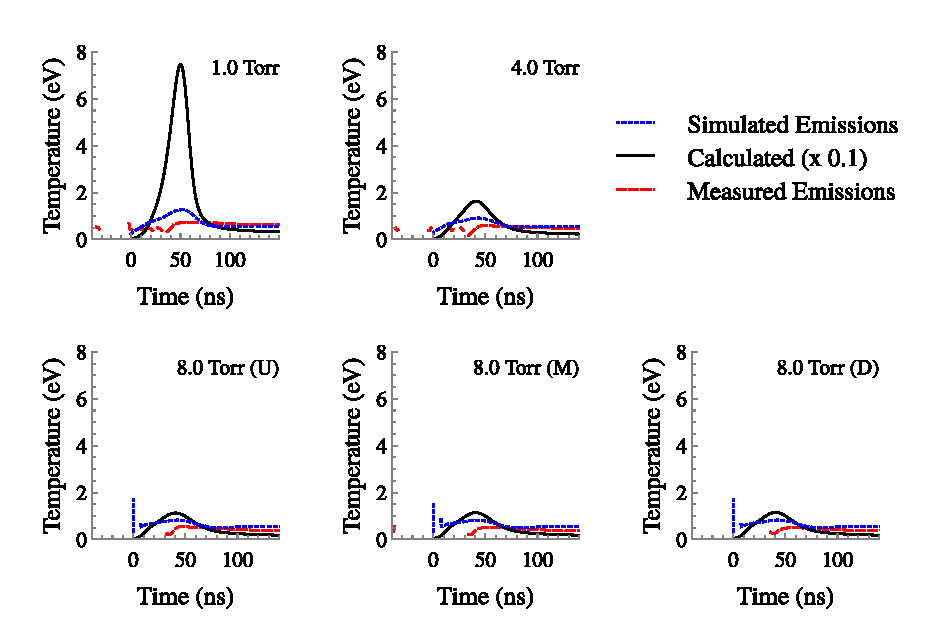
\includegraphics{./chapters/emissions/figures/boltcomp.eps}
  \caption{Temperatures estimated using Boltzmann plots of the measured emissions
    (dashed, red lines) and simulated emissions (dotted, blue lines) compared to
    the simulated temperatures (solid, black line).}
  \label{fig:boltcomp}
\end{figure}
Negligible plasma emissions occurred prior to the pulse, preventing any analysis
during that period of time. Estimates of the electron temperature using the
Boltzmann plot approach proved to provide poor predictions. Peak temperatures
were underestimated by at least a factor of ten, if not more. This disagreement
is not altogether unexpected--the assumption of equilibrium between the excited
states and the electrons is most certainly violated on such short time scales,
simply as a result of the finite time required for electron-atom collisions to
occur. This is confirmed by the poor quality of the temperature estimates
generated from the simulated emissions.

After the pulse, when the electrons are cooling primarily through elastic
collisions, it might be expected that the atomic state populations would relax
to an equilibrium distribution. While this is true for a long enough time
period, this behavior is not observed for the length of time under
consideration. Instead, the non-equilibrium distribution of atomic states that
is established during the pulse lasts well into the afterglow. As Kunze notes,
``one always has to check if indeed the assumption of a Boltzmann distribution
is justified \ldots, equilibrium may not be reached even if the steady-state
conditions seem to indicate that.'' \cite{Kunze2009}

Generally, the Boltzmann plots are poor predictors of the electron temperature
for the time period under consideration. This almost certainly results from the
inapplicability of the Boltzmann distribution to excited state populations. As
can be seen in figure~\ref{fig:boltex},
\begin{figure}
  \centering
  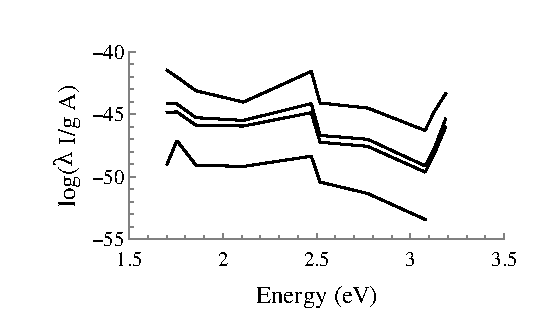
\includegraphics{./chapters/emissions/figures/boltex.eps}
  \caption{Boltzmann plot examples for the \acs{rpnd}}
  \label{fig:boltex}
\end{figure}
the plots show a large deviation from line that would be expected from theory.
To some extent, this too may be indicative of inaccuracies in the line intensity
measurements, however even after removing the transitions with relatively small
signals, no clear lines emerge. 

\subsection{Coronal Model}

In place of the assumption about an equilibrium distribution between excited
states, another approach is the use of the coronal model. In this case, the
states are considered to be excited by electrons, but to decay via optical
transitions. This model excels at low densities where states are not subject to
a great degree of mixing and inter-atomic collisions can be neglected. Again,
these assumptions do not necessarily apply to the \acs{rpnd}.

Per Kunze \cite{Kunze2009}, the line intensity ratio resulting from the coronal
model may be expressed as
\begin{equation}
  R = \frac{\lambda_{i',j'}A_{i,j}\sum A_{i'} K_{0,i}(T_e)}
  {\lambda_{i,j}A_{i',j'}\sum A_{i} K_{0,i'}(T_e)}
\end{equation}
where the sum is over all possible radiative decay pathways, the subscript `0'
is the ground state, and $K$ is the rate coefficient. Note that the rate
coefficients are explicitly functions of the electron temperature. The upper
states used for this line ratio must be carefully chosen so as to limit
sensitivity to collisional mixing of excited states. Likewise, the rate
coefficient ratio should exhibit a monotonic trend with electron temperatures.

Several ratios have been suggested by Kunze and others, including:
3$^3$S-2$^3$P$\odd$ over 3$^1$S-2$^1$P$\odd$, 4$^3$S-2$^3$P$\odd$ over
4$^1$S-2$^1$P$\odd$, and 4$^3$S-2$^3$P$\odd$ over 4$^1$D-2$^1$P$\odd$. The
ratios with the upper state in an S subshell are attractive as they are less
susceptible to collisional mixing between states of equal $n$ \cite{Kunze2009}.
However, the 4$^1$S-2$^1$P$\odd$ transition emissions were not recorded due to
their relatively low intensity. Likewise, the transitions for $n=3-2$ proved to
have too much noise for accurate line ratio measurements.

As a result, the only useful line ratio was 4$^3$S-2$^3$P$\odd$ over
4$^1$D-2$^1$P$\odd$. Like the other mentioned ratios, it is a comparison of
transitions in the triplet and singlet manifolds. Triplet-singlet ratios have
been found to be mostly dependent to electron temperature which makes them ideal
for this purpose \cite{Griem2005}. Figure~\ref{fig:conversion}
\begin{figure}
  \centering
  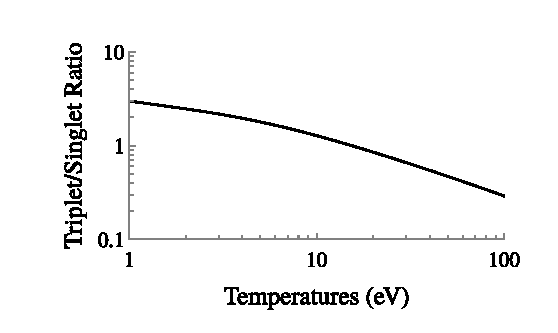
\includegraphics{./chapters/emissions/figures/conversion.eps}
  \caption{The emission ratio of 4$^3$S-2$^3$P$\odd$ over 4$^1$D-2$^1$P$\odd$ as
  a function of the electron temperature.}
  \label{fig:conversion}
\end{figure}
shows the relation between the emission intensity of the two transitions and the
electron temperature of the system. It should be noted that these ratios are
produced by rate coefficients calculated using a Maxwell-Boltzmann distribution.
While the measured ratios may be converted to a temperature by this process, it
remains to be seen whether it accurately represents the temperatures in the
\acs{rpnd}.

The calculated conversion between triplet-singlet ratio was used to estimate the
temperature of the \acs{rpnd} experiment in addition to the simulated emissions.
The results can be found in figure~\ref{fig:rat2comp}.
\begin{figure}
  \centering
  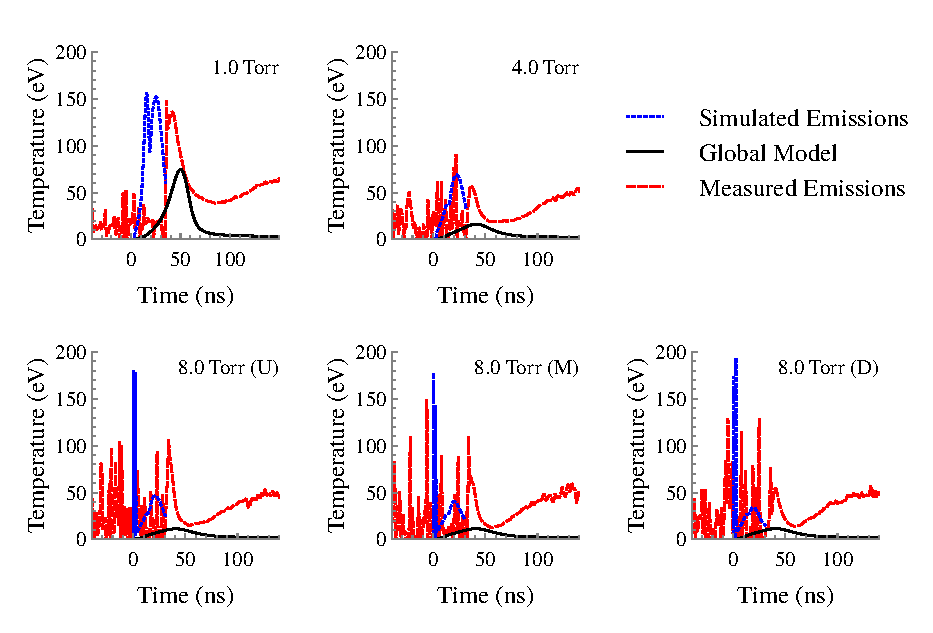
\includegraphics{./chapters/emissions/figures/rat2comp.eps}
  \caption{Estimates of the electron temperatures based on the ratio of the
    4$^3$S-2$^3$P$\odd$ and 4$^1$D-2$^1$P$\odd$ transitions. The estimates were
    generated for the simulated emissions (dotted, blue lines) and measured
    emissions (dashed, red lines), and are compared to the actual temperature
    results from the global model simulation (solid, black lines).}
  \label{fig:rat2comp}
\end{figure}
Generally, neither the simulated or measured ratios provide a good estimate of
the electron temperatures. Unlike the Boltzmann plots, both tend to overestimate
the temperature in the system, suggesting that the population ratio of the upper
states is different than expected. Furthermore, with the exception of the 1.0
Torr condition, the measured emission ratios predict higher temperatures than
the simulated emission ratios. This suggests an experimental excess of the
4$^1$D state, a deficit in the 4$^3$S state, or both. Of the two, it seems
likely that the 4$^1$D state is populated to a greater extent than simulated.
For one, the $n=5$ states are not included, and therefore the cascade from
higher states is not captured. Additionally, collisional mixing could serve to
increase the population of the D subshell compared to S subshell. Similar issues
with this particular ratio were recorded by Boivin et al. \cite{Boivin2007} who
suggested that improved data for the $n=5$ transitions could produce better
results.

Overall, these optical techniques appear to be of limited usefulness in the
determination of the electron temperature. As noted by Griem \cite{Griem2005},
even optimal experimental conditions have accuracies of 10\% in line intensity
measurements. Given the sensitive dependence of the calculated electron
temperature on the line ratio, as seen in figure~\ref{fig:conversion}, this
seemingly moderate inaccuracy can produce wildly varying results. This effect is
amplified as the absolute value of the emissions decline.

The use of the coronal model itself may not be relevant to the \acs{rpnd}. Kunze
\cite{Kunze2009} warns that coronal model may be invalid for large metastable
populations in helium. Additionally, the collisionality at the higher pressures
may also lead to a violation of the assumptions in the coronal model. For
example, the 3$^3$S-2$^3$P$\odd$ over 3$^1$S-2$^1$P$\odd$ ratio was considered
solely for the simulated emissions. Figure~\ref{fig:rat1comp}
\begin{figure}
  \centering
  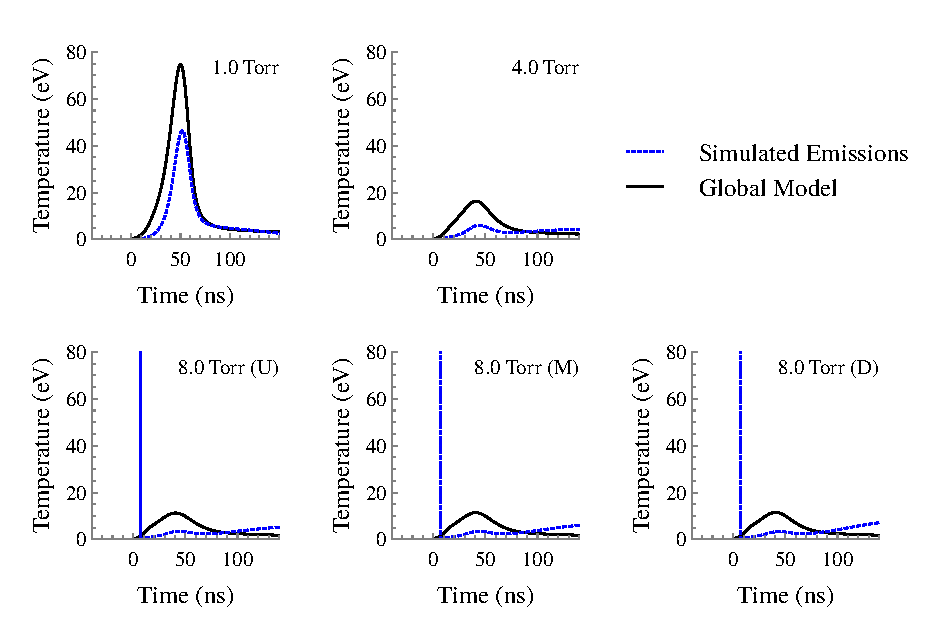
\includegraphics{./chapters/emissions/figures/rat1comp.eps}
  \caption{Estimates of the electron temperatures based on the ratio of the
    3$^3$S-2$^3$P$\odd$ over 3$^1$S-2$^1$P$\odd$ transitions. The estimates from
    the simulated emissions (dotted, blue lines) are compared to the temperatures
    from the global model.}
  \label{fig:rat1comp}
\end{figure}
shows that the results for this set of transitions are poor for most cases.
However, the agreement improves substantially for the 1.0 Torr case. This
appears to confirm the conclusion that the lack of agreement can, to some
degree, be attributed to the collisionality of the system and a violation of the
coronal model.

\section{Global Model Comparison}

In light of the disagreement between the line ratios in
figure~\ref{fig:rat2comp}, it is informative to consider a comparison of the
measured emission trends to the simulated emission trends. Deviations between
the two can likely be attributed to one of several causes: measurement error,
cross section accuracy, and distribution assumptions.

\section{Summary}


  \chapter{Conclusions}\label{chp:conclusions}
    The repetitively-pulsed nanosecond discharge \acs{rpnd} is a low temperature
plasma with several properties which make it amenable to novel applications.
Some of these properties include its production of a large uniform discharge (on
the order of liters), negligible gas heating, and operation over a wide range of
pressures \cite{Starikovskaia2001}. Though the \acs{rpnd} has only recently been
enabled by new semiconductor technology, it shares a long history with other
pulsed discharges. This includes the fast ionization wave (\acs{fiw}),
streamers, sparks, and lightning \cite{Loeb1965}.

Despite this long history, in-depth study of these phenomena has been
challenging. A review of the literature found that the important dynamics of the
\acs{rpnd}, which can occur in a matter of nanoseconds, were not well-explored.
This can be attributed to the time scales involved which present a number of
technical difficulties. Separately, the high electric fields and the substantial
collisionality within the \acs{rpnd} precludes the use of many traditional
plasma diagnostic techniques. Thus, most studies have focused on measurements of
the plasma properties after the pulse or averaged over the pulse.

However, as with most plasmas, the properties of the \acs{rpnd} are determined
by the coupling between the applied electric field and the gas. As this coupling
is a result of fundamental processes which occur during the nanosecond pulse,
such as electron acceleration and collisional excitation, the \acs{rpnd} can not
be understood without more detailed consideration of the dynamics which occur
during its initial phases.

\section{Overview of Results}

To that end, the necessary theory was developed to describe the \acs{rpnd}. This
began with the Boltzmann equation and Maxwell's equations, the basic equations
which can be used to describe any ionized gas. Several reductions of the
Boltzmann equation were presented in the form of moments. These moments averaged
over the velocity space of the probability distribution in order to simplify the
solution of the equations.

Following this, the criteria for a plasma were presented. A plasma is distinct
from an ionized gas in the sense that its behavior is dominated by its
electromagnetic properties. Thereafter, the initiation of a plasma from one or a
few electrons was explained for the two primary cases. The first, the Townsend
mechanism, occurs for relatively small electric fields, long periods of time,
and does not involve the formation of appreciable space charge. In contrast, the
streamer mechanism, involves a high electric field, develops over a shorter
period of time, and is influenced by the formation of large regions of space
charge.

It is the properties of the streamer mechanism which bear the most resemblance
to the \acs{rpnd}. However, the streamer model does not automatically account
for the uniform nature of the \acs{rpnd}. Instead, this was described by the
work of Levatter and Line \cite{Levatter1980}. They demonstrated that a streamer
can develop in a uniform manner provided a sufficient density of pre-pulse
electrons. Calculations for the subsequent experimental conditions found that
the natural electron density was sufficient to guarantee uniform breakdown at
all operating pressures. The theoretical discussion concluded with an
explanation of atomic structure, spectroscopic notation, and spectral
lineshapes.

Subsequently, an experimental \acs{rpnd} was described. It was generated by
repetitive positive voltage pulses in ultra-high purity helium at several
different pressures. The discharge geometry was of a coaxial design similar to
the \acs{fiw} studies reviewed by Vasilyak et al. \cite{Vasilyak1994}. Visual
observations and the ease with which breakdown was obtained suggested that the
plasma was most stable at a pressure of 4.0 Torr. However, estimates of the
energy coupling from the current-voltage measurements indicated that greatest
energy coupling occurred at 1.0 Torr, with a peak value of 5.5 mJ. This was
consistent with previous experimental measurements of the energy coupling in
\acs{rpnd}s and \acs{fiw}s.

Laser-absorption spectroscopy (\acs{las}) of the 2$^3$S, or triplet metastable,
state of helium was the primary means by which the nanosecond discharge dynamics
were measured. This technique produced measurements of the temperature and
line-integrated density of the triplet metastable state over the duration of the
pulse. The triplet metastable level because it can act as a large energy
reservoir in helium discharges and can increase the charged particle population
via associative ionization and Penning ionization. The use of an active optical
diagnostic, meant that the time resolution of the measurements were only limited
by the bandwidth of the detector, 5 ns.

The results of the \acs{las} confirmed that no gas heating was occurring in the
\acs{rpnd}. The accuracy of the temperature measurements varied with respect to
the metastable density, but was generally about $\pm50$ K. The largest detected
line-integrated densities, prior to the reflected pulse, occurred for the 4.0
Torr condition at a value of about 5.9$\times10^{16}$ m$^{-2}$. Assuming a
uniform density distribution across the discharge tube, this is equivalent to a
density of 1.8$\times10^{17}$ m$^{-3}$. A significant number of metastable atoms
persisted between pulses for pressures of 1.0 Torr and lower.

There were no observable trends in the metastable densities with respect to
axial location for pressures of 4.0 Torr and lower. This provides additional
confirmation of the homogeneous and volume-filling nature of the \acs{rpnd}. In
contrast, results at 8.0 and 16.0 Torr showed a clear decline in metastables
densities as a function of distance from the anode. This is believed to be akin
to the wave attenuation in \acs{fiw}s, described by Vasilyak et al.
\cite{Vasilyak1994}.

Long duration measurements of the metastable densities revealed the primary
decay processes in this discharge geometry. Metastable destruction at low
pressures was dominated by associative ionization; indicated by deviations from
a purely exponential decay. As the pressure of the system was increased, the
three-body reaction (leading to the formation of helium dimers) became the
dominant destruction process. Decay constants significantly larger than
those reported by Deloche et al. \cite{Deloche1976} and Phelps and Molnar
\cite{Phelps1953} suggest that gaseous impurities played a significant role in
metastable destruction.

A global model was then developed in order to infer various other plasma
parameters from the metastable measurements. The development of the model
included an analysis of the likely electron energy distribution functions
(\acs{eedf}s) in the \acs{rpnd} with a series of zero-dimensional
particle-in-cell (\acs{pic}) simulations. For fields of 100 Td and less, the
\acs{pic} simulations showed good agreement with Maxwell-Boltzmann distributions
of the same mean electron energy. However, above 300 Td, the Maxwell-Boltzmann
distributions exhibited significantly fewer high-energy (greater than 100 eV)
electrons. Better agreement with the \acs{pic} simulations at these field
strengths were obtained with solutions of the two-term expansion of the
Boltzmann equation. However, as a result of significant disagreements at lower
electric fields, the global model assumed a Maxwell-Boltzmann distribution for
the entirety of the simulations.

The global model simulations which best matched the measured metastable density
trends required the use of an exceptionally long electric field, 40 ns in
length, compared to the 25 ns length of the applied pulse. Upon inspection of
the optical emissions from the plasma, a return stroke was identified that
appeared to explain this longer-than-expected excitation. Based on previous
results in \acs{fiw} research \cite{Starikovskaia1998}, an alternative
explanation was also proposed in which a beam-like electron population formed in
the \acs{rpnd} and its relaxation was responsible for the extended excitation.

Using the long excitation period with the global model produced an excellent
match to the measured metastable densities, both during the pulse and afterward.
Particularly good agreement was obtained at 4.0 and 8.0 Torr conditions. Small
deviations were observed at 1.0 Torr--the metastable density appeared to rise
too quickly during the pulse, and too slowly after the pulse. This provided a
second hint that energetic electrons may be present in the system, specifically
at the lower pressure conditions.

This was reinforced by the magnitude of the electric fields and inferred
electron temperatures necessary to match the metastable densities. At 1.0 Torr,
the peak electric field was 346 Td and the peak electron temperature was
estimated at 74.6 eV. This suggests that the global model is likely inaccurate
for this condition given the disagreement between the Maxwell-Boltzmann
distribution and the \acs{pic} simulations at field values over 300 Td.
Additionally, the electron temperature is far in excess of what can be
considered reasonable for an equilibrium population of electrons in a low
temperature plasma.

In contrast, the global model predictions at 4.0 and 8.0 Torr were better
aligned with previously reported values. The electron temperatures are similar
to those recently obtained for a \acs{fiw} \cite{Takashima2011}, as well as
those predicted from rate coefficient calculations \cite{Aleksandrov2007}.
Likewise, the electric fields are more reasonable than those predicted at 1.0
Torr, though they fall in the intermediate region between 100 and 300 Td.

Interesting to note was a delay between the peak electric field and the highest
ionization rate in the plasma. This was interpreted as the time required for the
seed electron population to reach ionization-relevant temperatures. In a
simplified system, the ionization rate is an exponential function of time,
thus the density grows quickly thereafter.

The global model was designed to consider a total of 32 different species and
535 different reaction processes, including optical transitions. This provided
the opportunity to compare simulated plasma emissions generated by the global
model with those measured from the experimental \acs{rpnd}. Emission
measurements of the \acs{rpnd} covered ten detectable transitions in the
visible spectrum. These were used to estimate the wave velocities of the
\acs{rpnd}: 1.7-3.0$\times10^7$ m/s at 8.0 Torr, and 0.7-1.5$\times10^7$ at 16.0
Torr. All other conditions had wave velocities that were greater than
5$\times10^7$ m/s.

Afterward, an initial attempt was made to determine the evolution of the
electron temperature from a series of Boltzmann plots. The Boltzmann plots from
the simulated emissions and measured emissions both resulted in temperature
estimates of about 0.5-0.6 eV. The temperatures estimated from the simulated
emissions showed significant disagreement with the actual simulated
temperatures. This indicated that the use of Boltzmann plots for the \acs{rpnd}
is almost certainly flawed.

The reason for this lies in the assumption of partial local thermodynamic
equilibrium in the plasma. This requires that the excited state populations used
in the Boltzmann plot are in equilibrium with the electrons \cite{Kunze2009}.
However, the \acs{rpnd} likely develops too rapidly for this equilibrium to take
place. This conclusion was reinforced by an examination of the individual
Boltzmann plots for a series of times after the pulse.

Subsequently, an attempt was made to determine the electron temperature via a
coronal model and the use of line ratios \cite{Griem2005}. Three line ratios
were considered however one was immediately rejected for lack of detectable
emissions. The second, which compared the 4$^3$S-2$^3$P$\odd$ transition to the
4$^1$D-2$^1$P$\odd$ transition was used with little success. Estimates based on
the measured emissions produced unrealistic temperatures, and the estimates from
the simulated emissions did not agree with the actual temperatures from the
global model.

The second line ratio which compared the 3$^3$S-2$^3$P$\odd$ transition to the
3$^1$S-2$^1$P$\odd$ transition produced more promising results. The estimates
from the simulated emissions matched the global model temperatures, which
demonstrated that the line could potentially work provided the global model
results are applicable.

However, the estimates from the measured emissions were less successful. For
most points in time, the two transitions were too dim to obtain a reliable
ratio. In the cases that a temperature could be estimated, the results indicated
a peak electron temperature of about 5 eV, followed by a quick cooling to 0.5
eV. As the coronal model relies on the assumption of a Maxwell-Boltzmann
distribution, this approach will almost certainly produce misleading and
incorrect results at pressures of 1.0 Torr and below.

Additional comparisons were made between the simulated and measured emissions
for the 3$^1$D-2$^1$P$\odd$ transition, at 1.0, 4.0, and 8.0 Torr. Some general
features, such as the timing of the peak intensity, and the relative intensities
between pressures were consistent between the two. However the simulated
emissions generally decayed away faster after the peak intensity as compared to
the measured emissions. This suggested a prolonged excitation period in the
\acs{rpnd}, again hinting at the presence energetic electrons.

Furthermore, the decay rate of the measured emissions had a noticeable pressure
dependence. This suggested an atomic process was responsible, one which was not
accounted for in the global model. The metastable measurements suggested that
Penning ionization of impurities was an important loss mechanism. As a result,
it is believed likely that the 3$^1$D state was also affected by collisions with
gaseous impurities. This would explain the pressure dependence observed in the
measured emissions.

Finally, the effects of radiation trapping in the \acs{rpnd} were investigated
as another possible source of extended excitation. Observable effects of
radiation trapping were confirmed by a comparison of the simulated and measured
emissions from the 3$^1$P$\odd$-2$^1$S transition. Subsequent calculations
showed that the effective lifetime of the 3$^1$P$\odd$-1$^1$S transition could
be extended by a factor of nearly $10^5$ for the geometry in question. The
increased residence time of this energy increases the chance that it may be
transferred to another excited state or lead to ionization via collisions.
This suggests that radiation trapping in the \acs{rpnd} may lead to an increase
in the excited state and charged particle densities, similar to the metastable
states.

\section{Future Work}

There are several opportunities to improve on the work presented here. From an
experimental perspective, the metastable density measurements could be improved
by the use of a more sensitive detector. This would decrease the minimum
detectable metastable density and potentially provide pre-pulse metastable
densities for the other operating pressures. It would also be desirable to
revisit the existing metastable density measurements along various chords of the
discharge cylinder. This would provide radial density profiles via inversion
techniques.

The emission measurements could also stand to be improved by the use of a more
efficient grating, a more efficient photocathode, or both. These changes should
be made with measurement of the 706 and 728 nm lines in mind, as these appear to
be the most promising for transitions for use in optical electron temperature
measurements. Further improvements to the optical temperature measurements could
be made with the development of an appropriate collisional radiative model and
perhaps the use of alternative \acs{eedf}s in the calculation of the rate
coefficients.

The experiment could also be improved with the relatively simple addition of a
capacitive probe for sensing of the electric field within the plasma, similar to
that used by Takashima et al. \cite{Takashima2011}. The electric field
measurements would allow for confirmation of the return stroke which was
observed in the emissions data. The probe may also be used to determine if a
persistent electric field exists after the pulse.

The electric field information could then be incorporated into the global model
for more accurate predictions of the \acs{rpnd} properties. Other improvements
to the global model would include the addition of gas impurities and reactions
in response to the evidence that they contribute to the \acs{rpnd} dynamics.
Furthermore, the global model should be modified to include radiation trapping
effects for resonant transitions.

However, the global model is still fundamentally limited in how it handles the
\acs{eedf} within the \acs{rpnd}. This may be improved, to some extent, by the
inclusion of a Boltzmann solver. That said, the investigation of the \acs{eedf}s
suggests that the two-term expansion may not be sufficient for the fields in the
\acs{rpnd}. Another approach would be the use of a zero-dimensional \acs{pic}
model, similar to the one used in the \acs{eedf} calculations. It should be
possible develop such a code with the inclusion of the improved cross sections
of Ralchenko et al. \cite{Ralchenko2008} as well as the optical transitions from
Kramida \cite{Kramida2012}, with suitable alterations to account for trapping
effects. This approach would neatly sidestep the \acs{eedf} issues, however
there is the concern that this may lead to an excessively demanding
computational problem. Some simplification could be accomplished using a hybrid
method or by only using \acs{pic} calculations above certain field values.

\section{Final Remarks}

The experimental and simulation results presented represent one of the few
comprehensive attempts to analyze the nanosecond timescale dynamics of a
\acs{rpnd}. Several mechanisms, including the dynamics of the metastable
population and radiation trapping, have been identified which may influence the
evolution and stability of a helium \acs{rpnd}. In addition, evidence has been
provided for beam-like electrons at low operating pressures, and the effects of
impurities on the lifetimes of excited states.

Each of these phenomena represent an important component of how the nanosecond
pulse couples energy into a gas. In turn, it is the energy in that gas--the
electrons, ions, excited states, internal fields, and photons, which lends the
\acs{rpnd} its ability to purify water \cite{Malik2001}, sterilize surfaces
\cite{Ayan2009}, alter air flow \cite{Nishihara2007}, and generate nanoparticles
\cite{Ostrikov2011}. It is only through an improved understanding of how this
energy is distributed in a plasma that applications, such as these, can be
realized.


  \appendix
    \chapter{Measurements in an Air RPND}\label{chp:nasa}
      As early as 2001, researchers have proposed the use of a novel, hybrid engine
design for use in supersonic and hypersonic flight \cite{Macheret2001}. In some
ways similar to an earlier program \cite{Gurijanov1996}, it suggested that
magnetohydrodynamic (\acs{mhd}) accelerators were an enabling technology for
hypersonic transport. Briefly, a \acs{mhd} accelerator could be used to
simultaneously produce energy and slow the inlet airflow. This would allow the
use of a conventional turbojet engine at speeds well above its normal
operational range.

However, \acs{mhd} accelerators require an ionized fluid flow. Even at the high
altitudes associated with hypersonic flight, this is not easy to achieve.
Originally, Macheret suggested the use of electron beams, carefully tuned to
coincide with the peak in the ionization cross section in air. However, the use
of electron beams in the ionization of high pressure gases is accompanied by a
large number of technical issues, similar to those of some excimer lasers.
Therefore, in 2002, Macheret et al.\ proposed the use of a \acs{rpnd} to produce
an ``electron beam'' in situ \cite{Macheret2002} akin to the beams observed in
certain \acs{fiw} studies.

The use of a \acs{rpnd} is accompanied by a reduced ionization efficiency in
comparison to an electron beam. However, it reduces the some of the
implementation challenges and Macheret argued that it offered a more efficient
and stable option than breakdown with DC electric fields. Though the densities
of \acs{fiw}s in several air-related chemistries have been measured on several
occassions \cite{Anikin1998, Aleksandrov2007, Aleksandrov2008,
Starikovskaia2006}, similar studies do not appear to exist for \acs{rpnd}s in
air. Therefore, there is a need for electron density measurements to confirm
that \acs{rpnd}s are adequate for the \acs{mhd} accelerator requirements and to
quantify their ionization efficiency.

In addition, previous studies of \acs{fiw}s in air have observed fast gas
heating of molecular systems \cite{Popov2011}. Up to 40\% of the input energy
can be converted into translational energy through dissociation of oxygen and
quenching or electronically excited nitrogen states. As the \acs{rpnd} physics
are very similar to that of the \acs{fiw}, there is the possibility that it may
also cause fast gas heating. In combustion, this can play an important role in
the chemistry, flame holding, and ignition delay. More generally, gas heating
can impact material processing and ionization efficiency. As such, it is
important to develop reliable temperature diagnostics for \acs{rpnd}s in
molecular gases.

This appendix records the development of two diagnostics for an air \acs{rpnd}
at \acs{nasa} Glenn Research Center (\acs{grc}). Measurement of the electron
density was accomplished using millimeter-wave interferometry. Plasma
interferometry measures changes in the phase and amplitude of an electromagnetic
wave which has passed through the plasma \cite{Lieberman2005}. The phase shift
is proportional to the density of electrons while the change in amplitude is
related to the electron-neutral collision frequency. As with other wave-based
techniques, the density resulting from this approach is line integrated. The
translational temperature of the system was measured via

Translational temperatures were measured by analysis of the rotational spectra
associate with the second positive system of nitrogen. Rotational spectra result
from changes in the rotational quanta of a molecule. As the energy spacing of
the rotational levels is generally quite small (often on the order of $10^{-4}$
eV), inter-molecular collisions can easily redistribute them
\cite{Herzberg1950}. Provided enough collisions, the distribution of rotational
states should reflect the distribution of translational energy for the
molecules.

\section{Discharge Apparatus}

Experiments were conducted in a cylindrical vacuum chamber, reproduced in
figure~\ref{fig:nasachamber},
\begin{figure}
  \centering
  \setlength\fboxsep{0pt}
  \setlength\fboxrule{1.0pt}
  \fbox{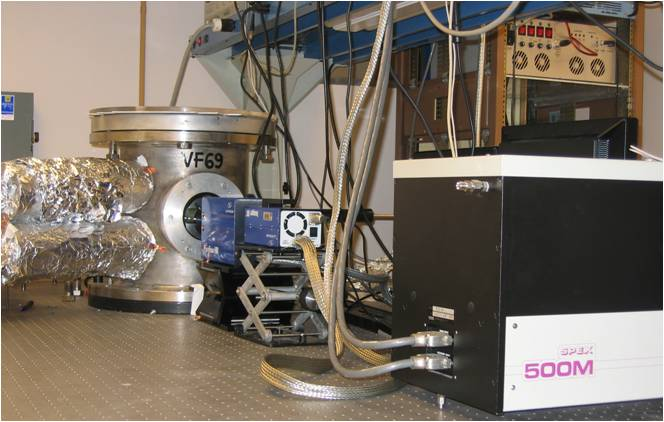
\includegraphics{./chapters/nasa/figures/VF-69.jpg}}
  \caption{Vacuum chamber used in \acs{rpnd} experiments at the \acs{nasa}
    \acs{grc} along with an \acs{iccd} used for fast imaging.}
  \label{fig:nasachamber}
\end{figure}
with a volume of approximately 30 L. The chamber was evacuated by a Varian
TriScroll 300, scroll pump and the pressure was monitored by a capacitance
manometer. Before each experiment the chamber pressure was reduced to below 100
mTorr, after which the chamber was sealed from the pump by a bellows valve. The
chamber was then back-filled with ambient air until the pressure reached 20.0
Torr.

The discharge was sustained between two parallel cylindrical electrodes, 2.5 cm
in diameter and 0.625 cm in length. In the interferometry experiment, the
electrodes were mounted in a silicone-based dielectric epoxy, cast such that it
was flush with the faces of the electrodes. Optical emission experiments
eliminated the dielectric epoxy in favor of a machinable ceramic and slightly
different geometry, seen in figure~\ref{fig:electrodes}.
\begin{figure}
  \centering
  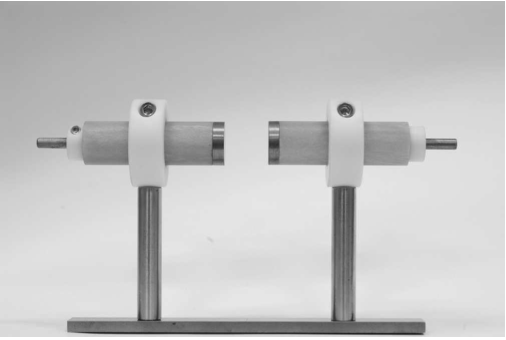
\includegraphics{./chapters/nasa/figures/electrodes.pdf}
  \caption{The electrodes used in the \acs{rpnd} at \acs{nasa} \acs{grc}. The
    electrodes are made of copper with a ceramic sheath made of Mykroy.}
  \label{fig:electrodes}
\end{figure}
This choice was made as a result of damage observed to the epoxy molds. Plasma
breakdown appeared to be occurring at the interface of the mold and the
electrodes. The use of the Mykroy fitting allowed longer duration operation
necessary for the optical emissions measurements.

The power supply was built by FID (model FPG 60-100-MC4-S5) and supplied voltage
pulses of up to 60 kV at repetition rates from 6-100 kHz with pulsewidths of 5
ns. Unless otherwise stated, all measurements were made with the power supply
operating at 20 kHz using a Wavetek FG3C as the master clock.

Maintenance of the electrodes and other components of the discharge apparatus
required that the chamber volume regularly be brought up to atmospheric
pressure. When the discharge was initiated after the chamber was returned to the
20.0 Torr operating pressure, a pressure transient was observed. This transient
caused the chamber pressure to rise by about 2.0 Torr after several minutes of
operation, after which the pressure would remain relatively stable. This was
believed to be caused by the outgassing of the discharge apparatus surfaces.
Throughout operation, the pressure would continue to increase at a greatly
reduced rate, on the order of several tenths of a Torr per minute.

\section{Millimeter-Wave Interferometry}

Traditionally, plasma interferometry has been conducted with microwaves, as the
electron densities in processing plasmas cause readily observable phase shifts
at these wavelengths. However, results from similar \acs{rpnd}s
\cite{Starikovskaia2001} suggested that the electron densities could approach
$10^{13}$ cm$^{-3}$. Such densities exceed the cutoff wavelength of microwave
interferometers \cite{Lieberman2005}. As a result, it was necessary to use
millimeter-wave (\acs{mmw}) interferometry which uses much higher frequencies in
order to avoid this issue.

\subsection{Theory}

The theory underlying interferometry can be found in many plasma diagnostic
textbooks, however the majority of the treatments only concern plasmas in which
there are no neutral particles. In contrast, the work of Akhtar et al.
\cite{Akhtar2003} introduces a frictional force to the derivation which accounts
for the effects of neutral particles. Following this approach, the theory below
provides the necessary set of equations in order to determine the electron
density and collision frequency provided measurements of the \acs{mmw} phase
shift and change in amplitude.

The derivation begins with the motion of electron in an oscillating
electromagnetic field. The position of a charged particle in such a field can be
found from the non-relativistic Lorentz equation,
  \begin{equation}
    \bm{F} = q\left( \bm{E} + \bm{v} \times \bm{B} \right),
    \label{eqn:lorentz}
  \end{equation}
where $\bm{F}$ is the force on the particle, $q$ is its charge, $\bm{E}$ is the
electric field, $\bm{v}$ is the particle's velocity, and $\bm{B}$ is the
magnetic field. In the case of a weak electromagnetic field (such as in
interferometry) the magnetic field component can be assumed to be zero. Without
loss of generality, the equation may be reduced to a single dimension.
Afterward, the drag force which accounts for the neutral particle collisions can
be introduced. The acceleration of the electron can then be written as
  \begin{equation}
    \ddot{r} = -\frac{e E}{m} - \nu_\mathrm{eff} m_e \dot{r},
  \end{equation}
where $r$ is the position of the electron, $e$ is the elementary charge,
$\nu_\mathrm{eff}$ is the effective rate of momentum transfer, and $m_e$ is the
mass of the electron.

A sinusoidal electric field can be expressed as $E_0 e^{i\omega t}$ where
$E_0$ represents the peak field strength and $\omega$ is the angular frequency.
The form of $E$ suggests a sinusoidal solution such that $r \propto e^{i\omega
t}$. Solving the differential equation for $\dot{r}$ yields
    \begin{equation}
        \dot{r} = -\frac{eE}{m_e}\frac{\nu_\mathrm{eff} + i\omega}
                                      {\nu_\mathrm{eff}^2 + \omega^2}.
    \end{equation}
This drift velocity can be used to solve for the complex plasma conductivity
and subsequently the dielectric constant. Finally, the complex propagation
constant can be written,
    \begin{equation}
        \gamma = \alpha + i\beta,
    \end{equation}
where $\alpha$ is the responsible for the amplitude decay and $\beta$ is
responsible for the phase shift. These are given by Akhtar as
    \newcommand{\ts}{\frac{\omega_p^2}{\omega^2 + \nu_\mathrm{eff}^2}}
    \begin{align}
        \beta & = \frac{\omega}{c} \left\{ \frac{1}{2} \left(1 - \ts \right)
                  + \frac{1}{2} \left[ \left( 1 - \ts \right)^2
                  + \left( \ts \frac{\nu_\mathrm{eff}}{\omega} \right)^2
                  \right]^{1/2} \right\}^{1/2}, \\
        \alpha & = \frac{\omega}{c} \left\{ -\frac{1}{2} \left(1 - \ts \right)
                   + \frac{1}{2} \left[ \left( 1 - \ts \right)^2
                   + \left( \ts \frac{\nu_\mathrm{eff}}{\omega} \right)^2
                   \right]^{1/2} \right\}^{1/2}.
    \end{align}
The electron density and collision frequency may be solved for explicitly such that
    \begin{align}
        \nu_\mathrm{eff} & = 2 \frac{c^2}{\omega}\frac{\alpha\beta}{\xi}, \\
        n_e & = \frac{m_e\epsilon_0}{e^2}\xi
                \left(\omega^2+\nu_\mathrm{eff}^2\right), 
    \end{align}
where $\xi = 1 - (\beta^2-\alpha^2)c^2/\omega^2$. The values for $\alpha$ and
$\beta$ come from experimental measures of the phase shift and change in
amplitude,
    \begin{align}
        \Delta \phi &= \int_0^d \left( \beta_0 - \beta\right)dr, \qquad
        \textrm{and} \\
        \Delta A &= \int_0^d \left( \alpha_0 - \alpha \right)dr,
    \end{align}
where $\Delta \phi$ is the phase change, $\Delta A$ is the amplitude change, $d$
is the pathlength through the plasma, and $\alpha_0$ and $\beta_0$ are free
space propagation values. As any measurements are integrated over the pathlength
of the system, it is common eliminate any spatial dependence by solving for
pathlength-averaged values.

pathlength-averaged values.

\section{Experiment}
    The mmW interferometry was conducted using an HP 8510C network analyzer operating at 75 GHz. The network analyzer was managed by a Labview script and had a maximum sample rate of 5 Hz. Each sample required approximately 100 $\mu$s to complete. The horns used to transmit and receive the mmW were align by maximizing the amplitude of the transmitted signal without the plasma present. The pathlength of the wave through the plasma was assumed to be 2.5 cm, however this is likely an underestimate as a result of diffusion.

    The actual operating pressures ranged from 19.9-22.6 Torr. The \textsc{fid} power supply was set up for bipolar operation at $\pm$9 kV with one electrode pulsed negative and the other positive. A DC sustainer discharge, as described in \cite{Schneider2009a}, was used in several cases. The sustainer is simply a set of electrodes perpendicular to the discharge axis of the \textsc{pnd}. The sustainer electrodes are held at a potential difference close to, but less than the DC breakdown voltage. The intended effect is an increase in ionization efficiency and a reduced recombination rate.
\section{Results}
    \subsection{Time Evolution}
        The first goal was to evaluate how the plasma changed over long periods of operation. The lack of a circulating air flow suggested that the discharge might change significantly from one minute to the next. This has significant implications for measurements that require acquisitions on the same time scale. One such example is gated passive spectroscopy; the light emitted by the \textsc{pnd} is extremely dim for sub-nanosecond measurements, making it necessary to accumulate light from several hundred or thousand individual pulses. Depending on the duty factor of the imaging device, such a measurement may require tens of minutes.

        The evolution of the plasma was captured over a period of 30 minutes. Longer duration acquisitions were limited by electromagnetic interference (\textsc{emi}) from the \textsc{pnd}. In particular, the master clock was particularly susceptible to interference. Despite extensive efforts to provide adequate shielding to the clock and all signal cables, a large number of experiments were halted as a result of this interference.

        \begin{figure}
            \centering
            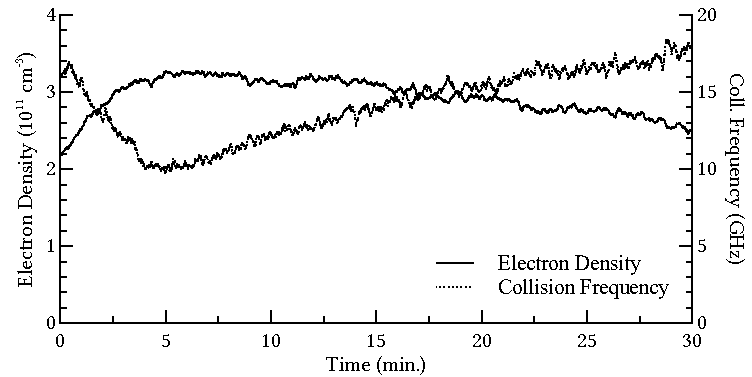
\includegraphics{./figures/densev.pdf}
            \caption{The evolution of the density (---) and the collision frequency (\raisebox{2.5pt}{${\scriptscriptstyle \centerdot \centerdot \centerdot}$}) in a \textsc{pnd} over a period of 30 minutes. These quantities reach their respective maximum and minimum after approximately five minutes, however these are not equilibrium values. The \textsc{pnd} continues to change over long durations.}\label{fig:densev}
        \end{figure}
        Figure \ref{fig:densev} shows a measurement of the density and collision frequency evolution over a period of thirty minutes for a \textsc{pnd} operating at 20 kHz, with applied voltages of $\pm$ 9 kV, and no DC sustainer. As hypothesized, there is an observable change in the average electron density on the order of minutes. It reaches a peak after five minutes, after which it shows a moderate decline. The collision frequency ranges from approximately 10-18 GHz. It reaches a minimum at five minutes, the same time that the electron density reaches its maximum, and subsequently rises. The actual average density ranged from approximately $2.25\times 10^{11}$ cm$^{-3}$ to $3.25\times 10^{11}$ cm$^{-3}$. The magnitude of the electron density is somewhat less than anticipated; other papers such as \cite{Aleksandrov2007}, \cite{Pancheshnyi1999}, and \cite{Macheret2006} state densities exceeding $10^{12}$ cm$^{-3}$. Separate experiments (not shown here) demonstrated similar electron densities and collision frequencies. However, the time for the system to reach its quasi-equilibrium varied and, in some cases, required 10 minutes.
        
        The observed increase in collision frequency was, perhaps, a result of increasing pressure and gas temperature in the chamber. Meanwhile, the change in electron density may be a result of a changing chemical composition. It is not immediately clear what mechanism is responsible for this, but it is well-known that electrons will readily attach to water molecules. As they are destroyed through dissociation, the attachment rate would decline and it would be reasonable to expect an increase in electron density.

    \subsection{DC Sustainer}
        Six separate experiments were run with the DC sustainer discharge on at approximately 750 V (current limited), and four experiments were run with the sustainer off (electrodes floating). Difficulties with \text{emi} prevented a more complete evaluation of the sustainer's effect. Therefore, an absolute statement on the influence of the DC sustainer is not possible. However, experiments without the DC sustainer exhibited consistently higher, but variable, densities.

        It is believed that the sustainer may have caused increased energy transfer to the excited states of atoms and molecules, but was ineffective at increasing the electron density. Indeed, the sustainer voltage was insufficient to produce a glow discharge independent of the high voltage pulses. As such, one may conclude that it will tend to extract more electrons than it produces. This being the case, a DC sustainer may be useful in situations requiring fast gas heating, but at the cost of a reduced ionization efficiency.

\section{Rotational Spectroscopy}

The approach used measured the rotational spectra of
a molecular system and used this information to infer the rotational
temperature. As a result of the close energy-spacing of the rotational levels,
this temperature is usually a good measure of the translational temperature of
the system \cite{Laux1993}. This technique is limited by the ability to detect
light from the transitions, and by the equilibration time of the translational
and rotational temperatures.

The measurement of rotational transitions is a common diagnostic for the
measurement of gas temperatures, particularly in the field of combustion.
Matching of the rotational spectra is typically accomplished with a computer
program such as Specair \cite{Laux2002} and LIFBASE \cite{Luque1999}. However, a
survey of the available programs revealed little documentation about the
calculation methods and none which provided the necessary flexibility how the
spectra were generated. This necessitated the development of a program to
automate the generation and matching of rotational spectra.


    \chapter{Laser-Absorption Analysis Code}\label{chp:lasana}
      The laser-absorption spectroscopy code was written in Python (version 2.7) using
the standard libraries, NumPy (version 1.6) and SciPy (version 0.11)
\cite{Jones2001}. The directory structure is as follows

%\dirtree{ %
%  .1 /. %
%  .2 analyze.py. %
%  .2 atoms. %
%  .3 __init__.py. %
%  .3 He.py. %
%  .2 gui.py. %
%  .2 lineshapes.py. %
%  .2 main.py. %
%  .2 models.py. %
%  .2 offset.py. %
%  .2 parse.py. %
%  .2 preprocess.py. %
%  .2 transition.py. %
%}

The analysis package can be initialized by running the command
\texttt{python main.py} from the root of the directory. This starts the
script which handles all of the settings, submodules, and main
processing loop. The code listing for \texttt{main.py} is as follows,

{\singlespacing
\lstinputlisting{./code/lasana/main.py}
}

It begins by importing several standard packages to manage directory names,
followed by the submodules and NumPy. Afterward, the transition class is used to
define the helium transitions of interest to the absorption analysis. The
variable names do not matter, but they do need to be compiled into a list called
\texttt{transitions} for use with the lineshape model.

The transition class is defined in the file \emph{transition.py}.

{\singlespacing
\lstinputlisting{./code/lasana/transition.py}
}

The class has no built in methods to speak of, instead it is merely acts as a
simple container for the transition information. Of some note is the fact that
it takes the vacuum wavelength and converts it to the air value.

After the main script defines the transitions, it initializes a graphical user
interface (\acs{gui}) 


    \chapter{Global Model Code}\label{chp:crammer}
      The global model code was written in Python (version 2.7) using the standard
libraries, NumPy (version 1.6), SciPy (version 0.11) \cite{Jones2001}, and
Matplotlib 1.3 \cite{Hunter2007}. The code will be included here for reference,
however the most up-to-date version will be maintained at
\url{https://github.com/l3enny/crammer}. Presently, the \texttt{conserve} branch
is the one that is in regular use, however its changes will eventually be merged
into the main branch. Below is a diagram of the directory structure used for the
global model code. Some additional files are present in the repository, but were
not used in producing the analysis presented here.

{
\dirtree{%
  .1 /. 
  .2 distributions.py. 
  .2 equilibrium. 
  .2 gases. 
  .3 \_\_init\_\_.py.
  .3 helium. 
  .4 \_\_init\_\_.py.
  .4 atomic.py.
  .4 constants.py.
  .4 optical.py.
  .4 states.py.
  .2 handler.py.
  .2 initcond.py.
  .2 matrixgen.py.
  .2 rates.py.
  .2 ratio.py.
  .2 script.py.
  .2 settings.
  .3 s1torr.py.
  .3 s4torr.py.
  .3 s8torr.py.
  .2 script.py.
  .2 solvers.py.
}
}

The global model is initialized by running the \texttt{script.py} file.
\begin{singlespace}
  \lstinputlisting{./code/crammer/script.py}
\end{singlespace}
As with the laser-absorption analysis code, this script mostly handles the logic
of the solutions and hands off the actual calculations to other libraries or
submodules. Aside from the importation of several submodules, the script
critically imports a settings file which determines much of how the solver
behaves. The settings file is intended to be much more straightforward to edit
in comparison to the solution script. An example of this is the settings file
for the 4.0 Torr conditions, \texttt{s4torr.py}.
\begin{singlespace}
  \lstinputlisting{./code/crammer/settings/s4torr.py}
\end{singlespace}
Because the main script imports all of the settings into its namespace, it is
important that the settings file define all of the variables listed in this
example. The settings file is generally well-commented, therefore little will be
said about the variables contained therein. The one notable exception is at the
beginning where two serialized objects (``pickles'') are loaded in to the
variables \texttt{km} and \texttt{coeffs}. As recorded in the comments,
\texttt{km} contains the function which generates the momentum transfer rate
coefficient. Similarly, \texttt{coeffs} contains the functions which generate
the electron-induced transition rate coefficients.

Both of these coefficient files are generated by a separate script, called
\texttt{rategen}. The function of this script will be described at the end of
this appendix. From an application standpoint, the \texttt{coeffs} function
accepts a float, and two integers as its inputs. The float is the electron
temperature in K, and the integers are unique identifiers of the excited atomic
state (in the form of $nSL$).

Finally, it should be noted that the settings file also imports a file called
\texttt{equilibrium.npy}. This file is generated by the settings file
\texttt{equilibrium.py} and contains the equilibrium values for the various
excited atomic states.

After the importation of the settings, the script also imports the states
information from the gas defined in the settings. It should be noted that the
\texttt{\_\_init\_\_.py} file in the gases directory contains a single line:
\texttt{\_\_all\_\_ = ['helium']}. This provides a hint to the Python runtime
about what submodules are included in the gases module. In this case, the gas is
helium, and the \texttt{states.py} file is recorded below.
\begin{singlespace}
  \lstinputlisting{./code/crammer/gases/helium/states.py}
\end{singlespace}
The states are contained in a single dictionary and referenced by their unique
integer indentifier. The energy of each state as well as its degeneracy is also
recorded here. Any commented state is automatically excluded from the
simulation.

After the states are imported by the script, an list is generated with their
indentifiers in order of energy. This is done because Python does not guarantee
the order of dictionaries. This order listing is later used for consistent
generation of the transition matrices. The transition matrices are produce by
the \texttt{matrixgen.py} submodule.
\begin{singlespace}
  \lstinputlisting{./code/crammer/matrixgen.py}
\end{singlespace}
This submodule contains all the function definitions necessary to generate the
various transition matrices. Conceptually, the row index is the same index as
the final state identifier in the \texttt{order} list. Likewise, the column
indicates the initial state index. The matrix generation functions automatically
track the losses and gains for each state and ensure conservation of particles.

After the transition matrices are generated, the \texttt{solvers.py} submodule
is used to generate the transition energies.
\begin{singlespace}
  \lstinputlisting{./code/crammer/solvers.py}
\end{singlespace}
This submodule does most of the calculations, though some of the functions (such
as the singular value decomposition) are wrappers for the SciPy equivalent. Also
in this submodule is a function which returns all the possible optical
transition wavelengths. Furthermore, two types of Runge-Kutta integrators are in
this submodule. The first is a simple fourth order method. The second implements
a fourth order method with a fifth order adaptive step size adjustment. The
latter of the two implements a generator pattern so that it could conceivably be
used without looping.

Returning to the main script, the differential equation describing the evolution
of the state density is set up, followed by the energy equation. Then, the
initial values are set up (based on the settings file), and the solution arrays
are initialized. This is followed by the solution loop which steps through the
evolution of the system and adjusts the rate coefficients as necessary. After
the end of the simulation period has been reached, the output files are opened
for writing, a process taken care of by \texttt{handler.py}.
\begin{singlespace}
  \lstinputlisting{./code/crammer/handler.py}
\end{singlespace}

As was mentioned earlier, the rate coefficients which are important to the use
of the global model are generated by a separate program and compiled into
serialized objects. The objects implement a \texttt{Rates} class which is
contained in \texttt{rates.py}.
\begin{singlespace}
  \lstinputlisting{./code/crammer/rates.py}
\end{singlespace}
The class acts as a data container for rate coefficients calculated at fixed
temperatures. It then implements a simple interpolating spline in order to
return appropriate rate coefficients as requested by the main script.

The \texttt{rategen} program can be accessed at the online repository,
\url{https://github.com/l3enny/rategen}. For the most part, it implements a
simple convolution routine around the transcribed cross sections and parses the
results into the above class. The contents of the \texttt{rategen} directory
include the listing below as well as several other files which are not necessary
for the analysis presented here.

{
\dirtree{%
  .1 /. 
  .2 settings.
  .3 combined.py.
  .3 pack1p0.py.
  .2 xsections.
  .3 \_\_init\_\_.py.
  .3 helium.
  .2 constants.py.
  .2 convolve.py. 
  .2 distributions.py. 
  .2 main.py.
  .3 rates.py.
}
}

The program begins with a call to \texttt{main.py}.
\begin{singlespace}
  \lstinputlisting{./code/rategen/main.py}
\end{singlespace}
This script begins with the necessary imports as well as the necssary imports,
most notably, the importation of the settings file. The settings file contains
the necessary information for the generation of the rate constants: temperatures
to use, type of distribution, comments, output name. Two examples follow, the
first, \texttt{combined.py}, was used to generate the electron-related rate
coefficients.
\begin{singlespace}
  \lstinputlisting{./code/rategen/settings/combined.py}
\end{singlespace}
In this case the cross sections and rates are imported from separate files
contained in the \texttt{xsections} directory. However, given the copyright on
these cross sections, this information is not reproduced here. The settings file
also imports the same \texttt{states.py} submodule as the \texttt{crammer}
script. Additionally, the settings import the distribution submodule,
\texttt{distributions.py}.
\begin{singlespace}
  \lstinputlisting{./code/rategen/distributions.py}
\end{singlespace}
This submodule includes a Maxwell-Boltzmann distribution, as well as a
two-factor distribution which is continuously variable between a Druyvesteyn
distribution and a Maxwell-Boltzmann.

After the settings are imported by the main script, it proceeds to assemble the
rate coefficients by convolving the selected distribution function with the
appropriate cross section. This is done via the \texttt{convolve.py} submodule.
\begin{singlespace}
  \lstinputlisting{./code/rategen/convolve.py}
\end{singlespace}
The convolve routine is a relatively simple numerical integration of the cross
section with That said, the maximum integration energy is hard-coded, therefore
the user should make the appropriate adjustments for reaction cross sections
and distribution functions with significant values past 100 eV. the distribution function. That said, the maximum integration
energy is hard-coded, therefore the user should make the appropriate adjustments
for reaction cross sections and distribution functions with significant values
past 100 eV.


    \chapter{Additional Emission Measurements}\label{chp:extraem}

  \bibliographystyle{unsrt}
  \bibliography{./Thesis}

\end{document}
